% !TeX encoding = UTF-8

\documentclass[UTF8,space=auto,xcolor=table,dvipsnames,svgnames,aspectratio=169]{ctexbeamer}
% Author: 2022 Log Creative <logcreative@outlook.com>
%         2021 Alexara Wu <alexarawu@outlook.com>

%% Use SJTUBeamer theme.
\usetheme[my,default,topright]{sjtubeamer}
\usemytheme{sjtug}
\setbeamertemplate{background}{}

%% If you don't use sjtubeamer theme.
%% Uncomment the following lines.
%% And use XeLaTeX to compile as well.
% \usetheme{nosjtubeamer}

\usepackage{fontawesome5}
\usepackage{hologo}
\usepackage{hyperxmp}
\usepackage{qrcode}
\usepackage{ulem}
\usepackage{subcaption}
\usepackage{booktabs}

\newcommand{\SJTUThesis}{\textsc{SJTUThesis}}
\newcommand{\SJTUThesisVersion}{1.1.0}
\newcommand{\SJTUThesisDate}{2022/3/26}
\newcommand{\SJTUBeamer}{\textsc{SJTUBeamer}}
\newcommand{\SJTUBeamerVersion}{2.6.1}
\newcommand{\SJTUBeamerDate}{2022/4/21}

\newcommand{\thesisissue}[1]{\href{https://github.com/sjtug/SJTUThesis/issues/#1}{\textsuperscript{\textcolor{.!90!DarkBlue}{\underline{\faCheckCircle{}#1}}}}}
\newcommand{\thesisdiscuss}[1]{\href{https://github.com/sjtug/SJTUThesis/discussions/#1}{\textsuperscript{\textcolor{.!90!DarkBlue}{\underline{\faComments{}#1}}}}}
\newcommand\link[1]{\href{#1}{\faLink}}
\newcommand\pkg[1]{\texttt{#1}}

\def\cmd#1{\texttt{\color{DarkBlue}$\backslash$#1}}
\def\env#1{\texttt{\color{DarkBlue}#1}}
\def\opt#1{\texttt{#1}}
\def\cls#1{\texttt{#1}}

%% Overleaf and some distributions omit the Adobe icon ...
%% If you need to display the Adobe logo, comment the following line.
\def\faAdobe{}

\lstset{
  escapechar=|
}

\newcommand{\includepdflarge}[1]{{\setlength{\fboxsep}{0pt}\framebox{\includegraphics[width=\linewidth,trim=4cm 17cm 3cm 2cm,clip]{#1}}\vspace{-10pt}}}
\newcommand{\includebeamerlarge}[2][1]{{\setlength{\fboxsep}{0pt}\framebox{\includegraphics[width=0.75\linewidth,page=#1]{#2}}}}

%% Use pympress to show the notes on the second screen.
% \setbeameroption{show notes on second screen}

\title{\LaTeX{} 新语}
\subtitle{上海交通大学图书馆专题培训讲座}
\author{李子龙}
\institute[SJTU Linux User Group]{上海交通大学 Linux 用户组}
\date{\the\year\,年\,\the\month\,月}
\subject{LaTeX, SJTUThesis, SJTUBeamer}

\hypersetup{
  pdfsubject         = {上海交通大学图书馆专题培训讲座},
  pdfauthor          = {Log Creative},
  pdfcopyright       = {Licensed under CC-BY-SA 4.0. Some rights reserved.},
  pdflicenseurl      = {http://creativecommons.org/licenses/by-sa/4.0/},
  unicode            = true,
  psdextra           = true,
  pdfdisplaydoctitle = true
}

\includeonly{
  support/contents/learnlatex,
  support/contents/sjtuthesis,
  support/contents/intermission,
  support/contents/sjtubeamer,
  support/contents/visualization,
  support/contents/boost
}

\begin{document}

% !TeX root = ../latex-talk.tex

\title{从零开始使用 \LaTeX{} 排版论文}
\subtitle{上海交通大学图书馆专题培训讲座}
\author{李子龙}
\institute[SJTU Linux User Group]{上海交通大学 Linux 用户组}
\date{2022 年 4 月}
\subject{LaTeX, 论文排版, SJTUThesis}
\maketitle

\begin{frame}{关于}
  \begin{columns}[c]
    \begin{column}{.7\textwidth}
      \begin{block}{从零开始使用 \LaTeX{} 排版论文}
        \alert{\url{https://github.com/sjtug/sjtulib-latex-talk}}
        
        \begin{flushleft}
          \small 本次讲座帮助学生从零开始跑起来 \LaTeX{},只用十步了解其基本概念和基础操作。学会使用 \textsc{SJTUThesis} 交大学位论文模板,并了解提升排版效率的相关技巧。
        \end{flushleft}

        \begin{tabular*}{0.8\linewidth}{@{\extracolsep{\fill}}lll@{}}
          \scriptsize 最后更新 & \scriptsize 幻灯片下载 & \scriptsize 许可证 \\
          \today & Overleaf \link{https://www.overleaf.com/read/fvwxzvcxhcwd} & \href{https://creativecommons.org/licenses/by-sa/4.0/}{\faCreativeCommons\,\faCreativeCommonsBy\,\faCreativeCommonsSa} \\ 
        \end{tabular*}
      \end{block}
      \vspace{0.2cm}
    \end{column}
    \begin{column}{.3\textwidth}
      \href{https://www.overleaf.com/read/fvwxzvcxhcwd}{
\includegraphics{support/figures/qrcode.pdf}}
    \end{column}
  \end{columns}
\end{frame}

\begin{frame}
  \frametitle{讲稿主要参考}
  \begin{bibliolist}{00}
    \onlineitem 陈晟祺~等.
    \newblock 如何使用 \LaTeX\ 排版论文[EB/OL].
    \newblock 2021. \url{https://github.com/tuna/thulib-latex-talk}.

    \onlineitem 曾祥东.
    \newblock 现代 \LaTeX\ 入门讲座[EB/OL].
    \newblock 2022. \url{https://github.com/stone-zeng/latex-talk}.

    \onlineitem \textsc{SJTUG}.
    \newblock \textsc{SJTUThesis} 用户文档[EB/OL].
    \newblock 2022. \url{https://github.com/sjtug/SJTUThesis}.

    \onlineitem \LaTeX\ Project.
    C\TeX\ 开发小组~译.
    \newblock learnlatex.org[EB/OL].
    \newblock 2022. \url{https://github.com/CTeX-org/learnlatex.github.io}.

    % \onlineitem \textsc{Oetiker T}, \textsc{Partl H}, \textsc{Hyna I}, \textsc{Schlegl E}.
    % C\TeX\ 开发小组~译.
    % \newblock 一份(不太)简短的 \LaTeXe{} 介绍:或 111 分钟了解 \LaTeXe{}[EB/OL]. \newblock\newblock 2021.
    % \url{https://ctan.org/pkg/lshort-zh-cn}.
  \end{bibliolist}
\end{frame}

% !TeX root = ../../latex-talk.tex

\part{学习 \LaTeX{}}
% FIXME: footnote fault numbering
% FIXME: section pop up in navigation in advance

\begin{frame}
  \frametitle{本部分主要参考}
  \begin{bibliolist}{00}
    \onlineitem 陈晟祺~等.
    \newblock 如何使用 \LaTeX\ 排版论文[EB/OL].
    \newblock 2021. \url{https://github.com/tuna/thulib-latex-talk}.

    \onlineitem 曾祥东.
    \newblock 现代 \LaTeX\ 入门讲座[EB/OL].
    \newblock 2022. \url{https://github.com/stone-zeng/latex-talk}.

    \onlineitem \LaTeX\ Project.
    \CTeX\ 开发小组~译.
    \newblock learnlatex.org[EB/OL].
    \newblock 2022. \url{https://github.com/CTeX-org/learnlatex.github.io}.
  
    \onlineitem \textsc{Oetiker T}, \textsc{Partl H}, \textsc{Hyna I}, \textsc{Schlegl E}.
    \CTeX\ 开发小组~译.
    \newblock 一份(不太)简短的 \LaTeXe{} 介绍:或 111 分钟了解 \LaTeXe{}[EB/OL]. \newblock\newblock 2021.
    \url{https://ctan.org/pkg/lshort-zh-cn}.
  \end{bibliolist}

  \note{推荐大家去阅读这些入门材料。}
\end{frame}

\begin{frame}[plain]
  \vfil
  \begin{center}
    \href{https://learnlatex.org}{
      \rmfamily
      Learn\,\lower1ex\hbox{\Huge\LaTeX{}}.org
    }
  \end{center}
  \vfil
  \begin{center}
    \parbox{0.75\linewidth}{
      Learn\LaTeX{}.org 提供了解 \LaTeX{} 的 16 篇简短的教程,并包含了一些可以在线运行的示例,可以通过亲自动手查看实验效果。本部分主要参考由 \CTeX{}-org 提供的中文翻译版本 \link{https://github.com/CTeX-org/learnlatex.github.io/tree/zh-Hans/zh-Hans/}。
    }
  \end{center}
  \vfil
  \note{这一部分主要参考了 Learn\LaTeX{}.org 的系列教程,内容简洁,适合入门,符合
  教育学观念 \link{https://www.tug.org/TUGboat/tb41-2/tb128reviews-learnlatex.pdf},
  并参考由 \CTeX{}-org 提供的中文翻译版本
  \link{https://github.com/CTeX-org/learnlatex.github.io/tree/zh-Hans/zh-Hans/}。
  如果你认为下面一个小时的入门教程没有讲得非常细致的话,
  欢迎直接阅读这个网站的全文。}
\end{frame}

\begin{shadedsection}

\section{是什么}
\begin{frame}
  \frametitle{\TeX{}}
  \begin{columns}[c]
    \begin{column}{0.7\textwidth}
      \begin{center}
        \rmfamily\Huge
        \hologo{La}\highlight[structure!70]{\TeX{}}
      \end{center}
      \begin{center}
        \parbox{0.75\textwidth}{
          \TeX{} 是由斯坦福大学教授高德纳
          (Donald E.~Knuth)于 1977 年开始开发的排版引擎。目前仍在更新,最新版本号为 3.141592653 \link{https://tug.org/TUGboat/tb42-1/tb130knuth-tuneup21.pdf}。
        }
      \end{center}
    \end{column}
    \begin{column}{0.3\textwidth}
      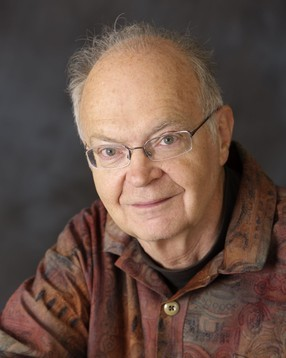
\includegraphics[width=.8\columnwidth]{support/images/Knuth.jpg}
    \end{column}
  \end{columns}
  \note{\emph{这一部分背景介绍大家可以了解一下,暂时跳过。}
  \LaTeX{} 这个词由两个部分组成,\hologo{La} 和 \TeX{}。那我们首先了解一下 \TeX{} 是什么。
  \TeX{} 是由斯坦福大学的教授高德纳于 1977 年开始开发的排版引擎,它已经有三十多年的历史了,
  目前仍在更新,版本号(3.141592653)将会趋近于 $\pi$ 的取值,高德纳最近还在给 \textsl{TUGBoat} 写稿子
  \link{https://tug.org/TUGboat/tb42-1/tb130knuth-tuneup21.pdf},
  关于 \TeX{} 今年又做了哪些改进。}
\end{frame}

\begin{frame}
  \frametitle{\LaTeX{}}
  \begin{columns}[c]
    \begin{column}{0.7\textwidth}
      \begin{center}
        \rmfamily\Huge
        \highlight[structure]{\LaTeX{}}
      \end{center}
      \begin{center}
        \parbox{0.75\textwidth}{
          \LaTeX{} 是最早在 1985 年由现就职于微软的 Leslie Lamport 开发的一种 \TeX{} \textbf{格式}\footnotemark,使用一些列宏和扩展宏包来简化 \TeX{} 的使用。现在由 \LaTeX{} Project 的成员维护。现在广泛使用的版本是 \LaTeXe{},最新的版本为 \LaTeX3(2020 年 10 月后默认内置)。
        }
      \end{center}
    \end{column}
    \begin{column}{0.3\textwidth}
      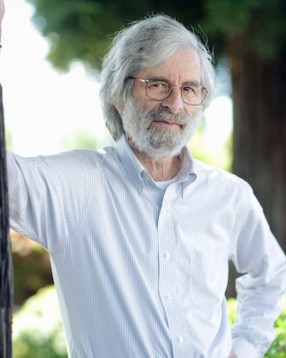
\includegraphics[width=.8\columnwidth]{support/images/Lamport.jpg}
    \end{column}
  \end{columns}
  \footnotetext{\hologo{ConTeXt} 也是一种 \TeX{} 格式 \link{https://www.contextgarden.net/}。}
  \note{\emph{这一部分的背景介绍大家可以了解一下,暂时跳过。}
  \LaTeX{} 是最早由现就职于微软的 Leslie Lamport 开发的一种 \TeX{} 格式(与其对标的是
  \hologo{ConTeXt}\link{https://www.contextgarden.net/}),主要也是为了简化 \TeX{} 的使用。
  现在主要由 \LaTeX{} 开发组维护,现在广泛使用的版本是 \LaTeXe{},最新的版本为 \LaTeX3,
  在 2020 年 10 月后默认内置,所以要尽可能使用较新的发行版,以充分发挥其功能。}
\end{frame}

\begin{frame}
  \frametitle{程序}
  \begin{columns}[c]
    \begin{column}{0.7\textwidth}
      \begin{center}
        \rmfamily\Huge
        \highlight[structure]{\hologo{pdfLaTeX}}
      \end{center}
      \begin{center}
        \parbox{0.7\textwidth}{
          \hologo{pdfLaTeX} 是为了编译一个 \LaTeX{} 文档而运行的程序。实际上底层在运行一个叫 \hologo{pdfTeX} 的引擎,并预装了对应的 \LaTeX{} \textbf{格式}。为了利用临时文件,可能就需要多次运行程序。
        }
      \end{center}
    \end{column}
    \begin{column}{0.3\textwidth}
      \begin{block}{}
        \ttfamily\small
        > \highlight{pdflatex} main.tex\\
        This is pdfTeX, Version 3.141592653-
        2.6-1.40.23 (MiKTeX 21.10)\\
        entering extended mode\\
        \highlight{LaTeX2e} <2021-11-15>\\
        \highlight{L3} programming layer <2021-11-22>
      \end{block}
    \end{column}
  \end{columns}
  \note{\hologo{pdfLaTeX} 是为了编译一个 \LaTeX{} 文档而运行的程序。}
\end{frame}

\begin{frame}
  \frametitle{引擎}
  \begin{columns}[c]
    \begin{column}{0.7\textwidth}
      \begin{center}
        \rmfamily\Huge
        \highlight[structure!70]{pdf}\hologo{La}\highlight[structure!70]{\TeX{}}
      \end{center}
      \begin{center}
        \parbox{0.7\textwidth}{
          pdf\TeX{} 是编译 \TeX{} 文档(以 \texttt{.tex} 结尾)的\textbf{引擎}---可以理解 \TeX{} 指令的\textbf{程序}。
        }
      \end{center}
    \end{column}
    \begin{column}{0.3\textwidth}
      \begin{block}{}
        \ttfamily\small
        > pdflatex main.tex\\
        This is \highlight[structure!70]{pdfTeX}, Version 3.141592653-
        2.6-1.40.23 (MiKTeX 21.10)
        entering extended mode\\
        LaTeX2e <2021-11-15>\\
        L3 programming layer <2021-11-22>
      \end{block}
    \end{column}
  \end{columns}
  \note{实际上底层在运行一个叫 \hologo{pdfTeX} 的引擎,并预装了对应的 \LaTeX{} 格式。}
\end{frame}

\begin{frame}[label={frame:engine}]
  \frametitle{Unicode 引擎}
  \begin{table}
    \caption{主流 \hologo{(La)TeX} 程序
    \footnote{(u)p\TeX{} 是日语最常用的引擎,生成 \texttt{.dvi},支持 Unicode。}\footnote{Ap\TeX{} \link{https://github.com/clerkma/ptex-ng} 具有底层 CJK 支持,内联 Ruby,Color Emoji。}}
    \footnotesize
    \begin{stampbox}
      \begin{tabular}{c>{\raggedright}*{3}{p{3.5cm}}}
        \alert{引擎}     & \hologo{pdfTeX}   & \hologo{XeTeX}   & \hologo{LuaTeX}   \\
        \alert{程序}     & \hologo{pdfLaTeX} & \hologo{XeLaTeX} & \hologo{LuaLaTeX} \\
        \alert{特点}     & 直接生成 PDF,支持 micro-typography  & 支持 Unicode、OpenType 与复杂文字编排 (CTL) & 支持 Unicode,内联 Lua,支持 OpenType \\
      \end{tabular}
    \end{stampbox}
  \end{table}

  \begin{center}
    \parbox{.9\textwidth}{
      \hologo{pdfLaTeX} 不支持 Unicode。为了排版中文,大部分情况下 \faApple{}\,\faLinux{} 应当使用 \hologo{XeLaTeX},而 \hologo{LuaLaTeX} 速度相对较慢。\faWindows{} 可以在一些情况下使用 \hologo{pdfLaTeX}。
    }
  \end{center}
  \note{当然为了排版中文,已经不再推荐使用 \hologo{pdfLaTeX} 了,应该使用 
  \hologo{XeLaTeX} 或者 \hologo{LuaLaTeX},当然后者的速度还是相对较慢,
  它们支持 Unicode 编码,并可以使用 OpenType 字体的全部功能。
  当然 \faWindows{} 平台下在某些追求速度的情况下,
  还是可以试着使用 \hologo{pdfLaTeX} 的。
  
  \hologo{LuaLaTeX} 理想情况下不慢,但是使用一些宏包后会破坏理想状态,
  也会因配置产生不同的结果,不同的操作系统在 I/O 速度上的不同也会导致不同的时间。

  \hologo{pdfLaTeX} 也支持,只不过需要先生成 tfm \TeX{} 字体度量文件,后续使用 \TeX{} 
  自身的配置方法,只能使用 7 比特或 8 比特字体。}
\end{frame}

% \begin{frame}
%   \paragraph{\hologo{pdfLaTeX}} \TeX{} 和 \LaTeX{} 被广泛使用之前,它们只需内置支持欧洲语言即可。在 Unicode 出现之前,\LaTeX{} 提供了许多种\textbf{文件编码}来允许很多语言的文字以原生的方式输入,\hologo{pdfLaTeX} 也只需要使用 8 位文件编码和 8 位字体。
% \end{frame}

\section{跑起来}
\begin{frame}
  \frametitle{发行版}
  \begin{table}
    \caption{\hologo{TeX} 发行版}
    \footnotesize
    \begin{stampbox}
      \begin{tabular}{c>{\raggedright}*{3}{p{3.2cm}}}
        \alert{发行版}     & \hologo{MiKTeX} \link{https://mirrors.sjtug.sjtu.edu.cn/ctan/systems/win32/miktex/setup/windows-x64/}   & \TeX{} Live \link{https://mirrors.sjtug.sjtu.edu.cn/ctan/systems/texlive/Images/}   & Mac\TeX{} \link{https://mirrors.sjtug.sjtu.edu.cn/ctan/systems/mac/mactex/}  \\[2pt]
        \alert{特点}      &  只安装必要文件,依赖用时更新  &  所有平台均可使用,每年发布一次 & Mac 系统专用,对 \TeX{} Live 的进一步打包 \\
        \alert{推荐平台}  & \faWindows  & \faLinux &  \faApple \\
      \end{tabular}
    \end{stampbox}
  \end{table}
  \begin{center}
    \parbox{.9\textwidth}{
      要让 \LaTeX{} 跑起来,核心就是要有一套 \TeX{} 发行版,来获取让 \LaTeX{} 工作所需的一组程序和文件。参考《一份简短的关于 \LaTeX{} 安装的介绍》\link{https://mirrors.sjtug.sjtu.edu.cn/ctan/info/install-latex-guide-zh-cn/install-latex-guide-zh-cn.pdf} 安装想使用的发行版。推荐使用发行版的最新版本\footnote{老版本 Linux 系统的包管理器自带 \TeX{} Live 发行版可能不是最新的 \link{https://repology.org/project/texlive/versions},尽量使用镜像安装,并手动将相关环境变量添加到路径 \link{https://www.tug.org/texlive/doc/texlive-zh-cn/texlive-zh-cn.pdf}。},并使用国内镜像。
    }
  \end{center}
  \note{要让 \LaTeX{} 跑起来,核心就是要有一套 \TeX{} 发行版,来获取让 
  \LaTeX{} 工作所需的一组程序和文件。参考《一份简短的关于 \LaTeX{} 安装的介绍》
  安装想使用的发行版,里面介绍了 \faWindows{}, \faApple{}, \faLinux{}, WSL 等系统上
  \TeX{} Live 的安装,非常全面,一步一步做就可以成功安装。目前最新的 \TeX{} Live 版本为
  2022,\SJTUThesis{} 用户不应当安装 \TeX{} Live 2020 以下的版本(后面会讲)。
  
  事实上,我认为这几个发行版各有操作系统偏好,虽然前两者是跨平台的。

  \hologo{MiKTeX} 对 Windows 用户较为友好,安装简单,占用空间不大,安装时间短,
  而且有完整的安装与卸载程序。可以给大家看一下 \hologo{MiKTeX} Console 的情况。

  \TeX{} Live 更符合 Linux 的更新传统。老版本 Linux 系统的包管理器自带 \TeX{} Live
  发行版可能不是最新的(到时间也会锁定依赖库的版本),尽量使用镜像安装(当然也推荐使用最新的
  Linux 发行版,这样它的版本也就一直是最新的),并手动将相关环境变量添加到路径。

  Mac\TeX{} 发行版有 pkg 安装包封装,并且附带了 \TeX{}Shop 基本编辑软件,更加适合 Mac OS。
  我用下来的话,感觉除了 \TeX{} Live Utility 外都有点过时了。}
\end{frame}

\begin{frame}[plain]
  \hbox to \textwidth{
    \hfil
    \vbox to 3cm{
      \hbox{
        \resizebox{3cm}{!}{
\includegraphics{support/examples/pics/sjtug}}
      }
    }
    \hfil
    \vbox to 3cm{
      \vfill
      \hbox{\Large\bfseries\color{structure} 稳定、快速、现代的镜像服务。}
      \vskip2pt
      \hbox{托管于华东教育网骨干节点上海交通大学。}
      \vfill
    }
    \hskip20pt
    \hfil
  }

  \begin{center}
    \parbox{0.8\textwidth}{
      推荐使用 SJTUG 软件镜像服务 \link{https://mirror.sjtu.edu.cn/},离得近,下得快。
      
      \begin{description}
        \footnotesize
        \item[\TeX{} Live]  {\ttfamily tlmgr option repository https://mirrors.sjtug.sjtu.edu.cn/CTAN/systems/texlive/tlnet}
        \item[\hologo{MiKTeX}] 在 \hologo{MiKTeX} Console 中设置镜像源为 \url{https://mirrors.sjtug.sjtu.edu.cn}
        \item[\faTelegram] 可以在 SJTUG 镜像站通知频道 \link{https://t.me/sjtug_mirrors_news} 获得更多信息,加入关联群组参与讨论。
      \end{description}
    }
  \end{center}
  \note{说到镜像,像后两者的安装包都很大(4GB 左右),由于一些原因,不采用镜像的话不知道要下到什么时候,对下载速度的要求高;
  而 \hologo{MiKTeX} 需要随时更新,宏包大小颗粒度大,对延迟的要求高。
  那么采用 SJTUG 镜像源将同时解决这两个问题,位于图信大楼的机房,凭借校内的高速网络,稳定快速下载,
  现在由 LightQuantum 维护的镜像站欢迎大家的使用,主页上还有更多的其他镜像可供使用,加入 Telegram 群组参与讨论。}
\end{frame}

\begin{frame}
  \frametitle{编辑器}
  \begin{table}
    \caption{开源编辑器推荐}
    \footnotesize
    \begin{stampbox}
      \begin{tabular}{c>{\raggedright}*{3}{p{3.5cm}}}
        \alert{编辑器}     & \begin{tabular}{c}Visual Studio Code \link{https://code.visualstudio.com}\\ \LaTeX{} Workshop\end{tabular}  & \TeX{}studio \link{https://texstudio.org} & \TeX{}works \\[5pt]
        \alert{特点}      &  搭配 VS Code 使用非常方便,易扩展  & 可以使用大量的菜单选项输入代码块,用户友好 & 只提供基础的高亮与运行方法,发行版自带\footnote{Mac\TeX{} 打包的是 \TeX{}Shop 编辑器。} \\
      \end{tabular}
    \end{stampbox}
  \end{table}
  \begin{center}
    \parbox{.9\textwidth}{
      使用专为 \LaTeX{} 设计的编辑器将带来更多便利,因为它们往往会提供一键编译、内置 PDF 阅读器以及语法高亮等功能。几乎所有现代的 \LaTeX{} 编辑器都提供 Sync\TeX{} 这一强大的功能,以在 PDF 和代码间对应跳转。
    }
  \end{center}
  \note{编辑器的种类很多,我无法一一列举,但是对编写 \TeX{} 常用的开源编辑器我推荐这三个。
  其中 \TeX{}studio 的安装包可能下得有点慢。这里我对这些编辑器都演示一下,初学者我更推荐使用
  \TeX{} studio 编辑器,如果平时就码很多代码的话,我更推荐使用 VS Code 加插件这种方式。
  
  使用专为 \LaTeX{} 设计的编辑器将带来更多便利,因为它们往往会提供一键编译、内置 PDF 阅读器
  以及语法高亮等功能。几乎所有现代的 \LaTeX{} 编辑器都提供 Sync\TeX{} 这一强大的功能
  (VS Code 的方法是 Ctrl + 某处,Overleaf 的方法是直接双击),以在 PDF 和代码间对应跳转。
  当然如果你不喜欢使用这种 GUI 编辑器,\TeX{} 文档本身就是纯文本,对 Vim, Emacs 等终端用户
  也很友好。}
\end{frame}

\begin{frame}
  \frametitle{在线平台}
  \begin{table}
    \caption{在线协作平台推荐}
    \footnotesize
    \begin{stampbox}
      \begin{tabular}{c>{\raggedright}*{2}{p{4cm}}}
        \alert{在线平台}     & Overleaf \link{https://www.overleaf.com/}  & 交大 \LaTeX{} 助手 \link{https://latex.sjtu.edu.cn/} \\[2pt]
        \alert{特点}      & 最流行的在线平台,提供大量的模板,但国内访问慢 & 校内平台,隐私保护有保障,共享项目限制少 \\
      \end{tabular}
    \end{stampbox}
  \end{table}
  \begin{center}
    \parbox{.9\textwidth}{
      在线平台允许你直接在网页中编辑文档,无需本地安装即可在后台运行 \LaTeX{},并显示生成的 PDF。可以参照 Overleaf 官方文档学习如何使用在线平台 \link{https://www.overleaf.com/learn}。
    }
  \end{center}
  \note{当然使用在线平台省去了安装发行版的麻烦,这里列出两种在线写作平台。

  如果有数据合规需求的话,可以考虑使用由网络信息中心维护的交大 \LaTeX{} 助手,最近更新了 \TeX{} Live 2022,还是很不错的。

  当然国内还有 \TeX{} Page \link{https://www.texpage.com/},Slagger \link{https://www.slager.cn/} 等。
  一般来讲,这种平台使用的都是 Linux 操作系统,所以在排版中文的时候考虑将编译引擎更改为 \hologo{XeLaTeX},
  学习如何使用在线平台参见 Overleaf 的官方文档 \link{https://www.overleaf.com/learn}。}
\end{frame}

\section{基本结构}
\begin{frame}[fragile]%
  \frametitle{文档部件}
  \begin{columns}[c]
    \begin{column}{0.4\textwidth}
      \only<1>{
        \cmd{documentclass} 命令加载了\textbf{文档类}。\cls{article} 是由 \LaTeX{} 提供的用于排版短文档的基本文档类。
        \begin{description}
          \footnotesize
          \item[\cls{article}] 不包含章的短文档
          \item[\cls{report}] 含有章的单面印刷文档
          \item[\cls{book}] 含有章的双面印刷文档
          \item[\cls{beamer}] 幻灯片
        \end{description}
      }

      \only<2>{
        \env{document} 环境用于指示文档主体的范围。\LaTeX{} 还有其他的使用 \cmd{begin} 和 \cmd{end} 的搭配,我们称这些为\textbf{环境}。它们将用来设定局部格式命令\footnotemark。
      }

      \only<3>{
        \includepdflarge{support/examples/enminimal.pdf}
      }
    \end{column}
    \begin{column}{0.6\textwidth}
      \begin{codeblock}[]{排版英文最简示例}
|\highlightline<1>|\documentclass{article}
|\highlightline<2>|\begin{document}
|\highlightline<3>|  Together for a Shared Future
|\highlightline<2>|\end{document}
      \end{codeblock}
    \end{column}
  \end{columns}

  \only<2>{\footnotetext{环境实际上是一个组,只不过通过语义化的形式预装了对应的格式命令。普通的组可以直接使用一对大括号之间的内容 \{$\cdots$\} 表示。}}
\end{frame}

\section{扩展}
\begin{frame}[fragile]%
  \frametitle{中文排版}
  \begin{columns}[c]
    \begin{column}{0.4\textwidth}

      \only<1>{
        \cmd{usepackage} 用于使用宏包以向 \LaTeX{} 添加或修改功能,需要在\textbf{导言区}调用。
        这里使用 \pkg{ctex} 宏集以获得中文支持。其调用底层因不同的引擎而不同。
        \begin{center}
          \footnotesize
          \begin{tabular}{c*{3}{c}}
            \alert{引擎}     & \hologo{pdfTeX}   & \hologo{XeTeX}   & \hologo{LuaTeX}   \\
            \alert{程序}     & \hologo{pdfLaTeX} & \hologo{XeLaTeX} & \hologo{LuaLaTeX} \\
            \alert{宏包}     & CJK\footnotemark & xeCJK & luatexja \\
            \alert{封装}     & \multicolumn{3}{c}{ctex} \\
          \end{tabular}
        \end{center}
        \vspace{-1cm}
      }

      \only<2>{
        \CTeX{} 建议对于之前提到的常规文档类,最佳实践是使用该宏集提供的四种中文文档类,以对特定类型提供额外的中文排版适配。
        \begin{center}
          \footnotesize
          \begin{tabular}{cc}
            \cls{ctexart} & \cls{ctexrep} \\
            \cls{ctexbook} & \cls{ctexbeamer} \\
          \end{tabular}
        \end{center}
      }

      \only<3>{
        \includepdflarge{support/examples/cnminimal.pdf}
      }

      \only<4>{
        大部分情况下,你都不应当在 \LaTeX{} 中强制断行:你几乎只是想另起一段,或者是想在段落之间添加空行(使用 \pkg{parskip} 宏包就可实现)。
        只有\alert{很少的}情况下你需要使用 \textbackslash{}\textbackslash{} 来另起一行而不另起一段(强制断行仍在同一段)。
      }
    \end{column}
    \begin{column}{0.6\textwidth}
      \begin{codeblock}[]{排版中文\only<2->{最佳实践}}
|\highlightline<2>|\documentclass{|\only<1>{article}\only<2->{ctexart}|}
|\only<1>{\highlightline\textbackslash{}usepackage\{ctex\}\hfill\color{structure}\% 导言区}|
\begin{document}
|\highlightline<3>|    一起向未来
|\highlightline<4>|
  Together for a Shared Future
\end{document}
      \end{codeblock}
    \end{column}
  \end{columns}
  \only<1>{\footnotetext{ctex 在 \faApple\,\faLinux{} 上已经不可以使用 \hologo{pdfLaTeX} 编译,以及在 \faWindows{} 上使用该引擎也会变更自动间距调整等功能的默认行为。}}
\end{frame}

\section{设定格式}
\begin{frame}[fragile]%
  \frametitle{字体样式}
  \begin{columns}
    \begin{column}{0.4\textwidth}
      \only<1>{
        \includepdflarge{support/examples/fontstyle.pdf}
      }

      \only<2>{
        可以使用显式样式设定命令对小段做加粗、斜体、等宽等等的处理。
        \begin{center}
          \footnotesize
          \begin{tabular}{rl}
            \cmd{textrm} & \textrm{衬线} \\
            \cmd{textbf} & \textbf{加粗} \\
            \cmd{textit} & \kaishu 斜体 \\
            \cmd{texttt} & \texttt{等宽} \\
            \cmd{textsf} & \textsf{无衬线} \\
            \cmd{textsc} & \textsc{Small Caps} \\
            \cmd{textsl} & \textsl{Slanted} \\
          \end{tabular}
        \end{center}
      }

      \only<3>{
        与 Word 不同的是,\LaTeX{} 一般情况下并不需要使用上面的显式命令,而是采用逻辑标记的方法,
        比如 \cmd{emph} 可以强调文字,以及下面将要提到的目次命令(第 \ref{sectioning} 页)。
        这样可以统一管理格式。
      }
    \end{column}
    \begin{column}{0.6\textwidth}
      \begin{codeblock}[]{样式}
\documentclass{ctexart}
\begin{document}
|\highlightline<2>|  \textbf{|\phantom{}|一起向未来}

|\highlightline<3>|  \emph{Together for a Shared Future}
\end{document}
      \end{codeblock}
    \end{column}
  \end{columns}
\end{frame}

\begin{frame}[fragile]%
  \frametitle{\only<1-2>{字体大小}\only<3>{字体样式}}
  \begin{columns}
    \begin{column}{0.4\textwidth}
      \only<1>{
        \includepdflarge{support/examples/fontsize.pdf}
      }

      \only<2>{
        同样地,你也可以显式地设定字体大小,但是这种命令会更改行文设置,所以需要使用一个组来限定作用范围\footnotemark。
        \begin{center}
          \footnotesize
          \begin{tabular}{rl}
            \cmd{tiny} & \tiny 极小 \\
            \cmd{scriptsize} & \scriptsize 角标大小  \\
            \cmd{footnotesize} & \footnotesize 脚注大小 \\
            \cmd{small} & \small 小 \\
            \cmd{normalsize} & \normalsize 正常大小 \\
            \cmd{large} & \large 大 \\
            \cmd{huge} & \Huge 巨大 \\
          \end{tabular}
        \end{center}
      }

      \only<3>{
        也可以使用字体样式对应的更改字体设置的命令,这对于大段文段的设置而言也是很方便的。
        \begin{center}
          \footnotesize
          \begin{tabular}{ll}
            \cmd{textrm} & \cmd{rmfamily}\\
            \cmd{texttt} & \cmd{ttfamily}\\
            \cmd{textsf} & \cmd{sffamily}\\
            \cmd{textbf} & \cmd{bfseries}\\
            \cmd{textit} & \cmd{itshape}\\
            \cmd{textsc} & \cmd{scshape}\\
            \cmd{textsl} & \cmd{slshape}\\
          \end{tabular}
        \end{center}
      }
    \end{column}
    \begin{column}{0.6\textwidth}
      \begin{codeblock}[]{大小}
\documentclass{ctexart}
\begin{document}
|\highlightline<2>|  {\bfseries\Large 一起向未来\par}
|\highlightline<3>|  {\itshape Together for a Shared Future}
\end{document}
      \end{codeblock}
    \end{column}
  \end{columns}

  \only<2>{\footnotetext{注意最后显式地使用 \cmd{par} 在改回大小前结束该段,否则会导致下一行的行间距异常!}}
\end{frame}

\section{逻辑结构}
\begin{frame}[fragile]
  \frametitle{列表}
  \begin{columns}
    \begin{column}{0.35\textwidth}
      \begin{codeblock}[]{无序列表}
\documentclass{ctexart}
\begin{document}
|\highlightline|  \begin{itemize}
    \item 第一项
    \item 第二项
    \item 第三项
|\highlightline|  \end{itemize}
\end{document}
      \end{codeblock}
    \end{column}
    \begin{column}{0.35\textwidth}
      \begin{codeblock}[]{有序列表}
\documentclass{ctexart}
\begin{document}
|\highlightline|  \begin{enumerate}
    \item 第一项
    \item 第二项
    \item 第三项
|\highlightline|  \end{enumerate}
\end{document}
      \end{codeblock}
    \end{column}
    \begin{column}{0.35\textwidth}
      \begin{codeblock}[]{描述列表}
\documentclass{ctexart}
\begin{document}
|\highlightline|  \begin{description}
    \item[|\phantom{}|第一] 文本
    \item[|\phantom{}|第二] 文本
    \item[|\phantom{}|第三] 文本  
|\highlightline|  \end{description}
\end{document}
      \end{codeblock}
    \end{column}
  \end{columns}
  \note{接下来我们概览一下三种列表:无序列表、有序列表、描述列表。这些列表可以相互嵌套,但最多嵌套四层。}
\end{frame}

%更深的列表技巧,定理环境等

\begin{frame}
  \frametitle{列表}
  \begin{columns}
    \begin{column}{0.35\textwidth}
      \includepdflarge{support/examples/unordered.pdf}
    \end{column}
    \begin{column}{0.35\textwidth}
      \includepdflarge{support/examples/ordered.pdf}
    \end{column}
    \begin{column}{0.35\textwidth}
      \includepdflarge{support/examples/description.pdf}
    \end{column}
  \end{columns}
\end{frame}

\begin{frame}[fragile,label=sectioning]%
  \frametitle{目次结构}
  \begin{columns}
    \begin{column}{0.4\textwidth}
      \LaTeX{} 可以使用目次命令将文档划分层级\footnotemark,并自动设定对应字体样式和大小。
      \begin{center}
        \footnotesize
        \begin{tabular}{rll}
          命令 & 含义 & 层次 \\
          \cmd{chapter} & 章\footnotemark & \sout{0} \\
          \cmd{section} & 节 & 1 \\
          \cmd{subsection} & 小节 & 2 \\
          \cmd{subsubsection} & 小小节 & 3 \\
        \end{tabular}
      \end{center}
    \end{column}
    \begin{column}{0.6\textwidth}
      \begin{codeblock}[]{目次}
\documentclass{ctexart}
\begin{document}
|\highlightline|  \section{|\phantom{}|概念}
|\highlightline|  \subsection{\LaTeX{}}
  \LaTeX{} 是一个用以排版高质量作品的文档准备系统。
\end{document}
      \end{codeblock}
    \end{column}
  \end{columns}
  \footnotetext{章这一级只在 \cls{report} 和 \cls{book} 文档类(包括对应的中文文档类)有定义。还有不常用的 \cmd{part} (0@\cls{article}/-1@\cls{report}\&\cls{book}\&\cls{beamer}) 以及更低层次的 \cmd{paragraph} (4) 与 \cmd{subparagraph} (5)。 }
  \note{而知道层次,对我们下面生成目录有帮助。}
\end{frame}

\begin{frame}[fragile]%
  \frametitle{组织文档}
  \begin{columns}
    \begin{column}{0.4\textwidth}

      \only<1>{
        \cmd{tableofcontents} 用来生成对于目次命令的目录。如果你想设定显示到哪个层级,在这个命令前使用 \cmd{setcounter\{tocdepth\}\{层次\}}

        如果你想在目录中使用更短的标题:

            \cmd{section[短标题]\{长标题\}}

        如果你想让本目次的标题不显示在目录中:

            \cmd{section*\{目录没这个标题\}}
      }

      \only<2>{
        对于大型文档而言,使用多个文件管理源文件通常是更方便的。而 \cmd{include} 和 \cmd{input} 都以相对路径的方式插入其他 \TeX{} 文档。
        区别在于,\cmd{include} 命令会从新页开始并做一些内部调整,这基本上只对 \pkg{chapter} 这一级有用。而 \cmd{input} 会原样插入源代码。
      }

      \only<3>{
        但是 \cmd{include} 插入的文档可以使用 \cmd{includeonly} 管理当前要排印哪一部分的内容,利用所有章节辅助文件的同时,减少编译时间并专注于该部分的内容。
      }
    \end{column}
    \begin{column}{0.6\textwidth}
      \begin{codeblock}[]{主文档}
\documentclass{ctexrep}
|\highlightline<3>|\includeonly{learnlatex,sjtuthesis}
\begin{document}
|\highlightline<1>|  \tableofcontents
|\only<2-3>{\highlightline}|  % !TeX root = ../../latex-talk.tex

\part{学习 \LaTeX{}}
% FIXME: footnote fault numbering
% FIXME: section pop up in navigation in advance

\begin{frame}
  \frametitle{本部分主要参考}
  \begin{bibliolist}{00}
    \onlineitem 陈晟祺~等.
    \newblock 如何使用 \LaTeX\ 排版论文[EB/OL].
    \newblock 2021. \url{https://github.com/tuna/thulib-latex-talk}.

    \onlineitem 曾祥东.
    \newblock 现代 \LaTeX\ 入门讲座[EB/OL].
    \newblock 2022. \url{https://github.com/stone-zeng/latex-talk}.

    \onlineitem \LaTeX\ Project.
    \CTeX\ 开发小组~译.
    \newblock learnlatex.org[EB/OL].
    \newblock 2022. \url{https://github.com/CTeX-org/learnlatex.github.io}.
  
    \onlineitem \textsc{Oetiker T}, \textsc{Partl H}, \textsc{Hyna I}, \textsc{Schlegl E}.
    \CTeX\ 开发小组~译.
    \newblock 一份(不太)简短的 \LaTeXe{} 介绍:或 111 分钟了解 \LaTeXe{}[EB/OL]. \newblock\newblock 2021.
    \url{https://ctan.org/pkg/lshort-zh-cn}.
  \end{bibliolist}

  \note{推荐大家去阅读这些入门材料。}
\end{frame}

\begin{frame}[plain]
  \vfil
  \begin{center}
    \href{https://learnlatex.org}{
      \rmfamily
      Learn\,\lower1ex\hbox{\Huge\LaTeX{}}.org
    }
  \end{center}
  \vfil
  \begin{center}
    \parbox{0.75\linewidth}{
      Learn\LaTeX{}.org 提供了解 \LaTeX{} 的 16 篇简短的教程,并包含了一些可以在线运行的示例,可以通过亲自动手查看实验效果。本部分主要参考由 \CTeX{}-org 提供的中文翻译版本 \link{https://github.com/CTeX-org/learnlatex.github.io/tree/zh-Hans/zh-Hans/}。
    }
  \end{center}
  \vfil
  \note{这一部分主要参考了 Learn\LaTeX{}.org 的系列教程,内容简洁,适合入门,符合
  教育学观念 \link{https://www.tug.org/TUGboat/tb41-2/tb128reviews-learnlatex.pdf},
  并参考由 \CTeX{}-org 提供的中文翻译版本
  \link{https://github.com/CTeX-org/learnlatex.github.io/tree/zh-Hans/zh-Hans/}。
  如果你认为下面一个小时的入门教程没有讲得非常细致的话,
  欢迎直接阅读这个网站的全文。}
\end{frame}

\begin{shadedsection}

\section{是什么}
\begin{frame}
  \frametitle{\TeX{}}
  \begin{columns}[c]
    \begin{column}{0.7\textwidth}
      \begin{center}
        \rmfamily\Huge
        \hologo{La}\highlight[structure!70]{\TeX{}}
      \end{center}
      \begin{center}
        \parbox{0.75\textwidth}{
          \TeX{} 是由斯坦福大学教授高德纳
          (Donald E.~Knuth)于 1977 年开始开发的排版引擎。目前仍在更新,最新版本号为 3.141592653 \link{https://tug.org/TUGboat/tb42-1/tb130knuth-tuneup21.pdf}。
        }
      \end{center}
    \end{column}
    \begin{column}{0.3\textwidth}
      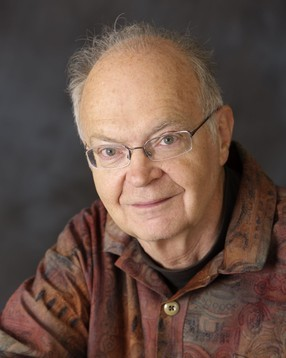
\includegraphics[width=.8\columnwidth]{support/images/Knuth.jpg}
    \end{column}
  \end{columns}
  \note{\emph{这一部分背景介绍大家可以了解一下,暂时跳过。}
  \LaTeX{} 这个词由两个部分组成,\hologo{La} 和 \TeX{}。那我们首先了解一下 \TeX{} 是什么。
  \TeX{} 是由斯坦福大学的教授高德纳于 1977 年开始开发的排版引擎,它已经有三十多年的历史了,
  目前仍在更新,版本号(3.141592653)将会趋近于 $\pi$ 的取值,高德纳最近还在给 \textsl{TUGBoat} 写稿子
  \link{https://tug.org/TUGboat/tb42-1/tb130knuth-tuneup21.pdf},
  关于 \TeX{} 今年又做了哪些改进。}
\end{frame}

\begin{frame}
  \frametitle{\LaTeX{}}
  \begin{columns}[c]
    \begin{column}{0.7\textwidth}
      \begin{center}
        \rmfamily\Huge
        \highlight[structure]{\LaTeX{}}
      \end{center}
      \begin{center}
        \parbox{0.75\textwidth}{
          \LaTeX{} 是最早在 1985 年由现就职于微软的 Leslie Lamport 开发的一种 \TeX{} \textbf{格式}\footnotemark,使用一些列宏和扩展宏包来简化 \TeX{} 的使用。现在由 \LaTeX{} Project 的成员维护。现在广泛使用的版本是 \LaTeXe{},最新的版本为 \LaTeX3(2020 年 10 月后默认内置)。
        }
      \end{center}
    \end{column}
    \begin{column}{0.3\textwidth}
      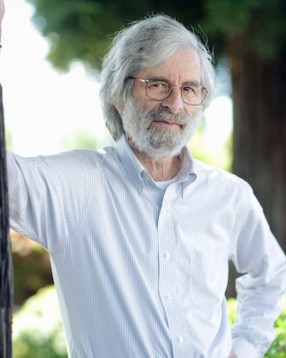
\includegraphics[width=.8\columnwidth]{support/images/Lamport.jpg}
    \end{column}
  \end{columns}
  \footnotetext{\hologo{ConTeXt} 也是一种 \TeX{} 格式 \link{https://www.contextgarden.net/}。}
  \note{\emph{这一部分的背景介绍大家可以了解一下,暂时跳过。}
  \LaTeX{} 是最早由现就职于微软的 Leslie Lamport 开发的一种 \TeX{} 格式(与其对标的是
  \hologo{ConTeXt}\link{https://www.contextgarden.net/}),主要也是为了简化 \TeX{} 的使用。
  现在主要由 \LaTeX{} 开发组维护,现在广泛使用的版本是 \LaTeXe{},最新的版本为 \LaTeX3,
  在 2020 年 10 月后默认内置,所以要尽可能使用较新的发行版,以充分发挥其功能。}
\end{frame}

\begin{frame}
  \frametitle{程序}
  \begin{columns}[c]
    \begin{column}{0.7\textwidth}
      \begin{center}
        \rmfamily\Huge
        \highlight[structure]{\hologo{pdfLaTeX}}
      \end{center}
      \begin{center}
        \parbox{0.7\textwidth}{
          \hologo{pdfLaTeX} 是为了编译一个 \LaTeX{} 文档而运行的程序。实际上底层在运行一个叫 \hologo{pdfTeX} 的引擎,并预装了对应的 \LaTeX{} \textbf{格式}。为了利用临时文件,可能就需要多次运行程序。
        }
      \end{center}
    \end{column}
    \begin{column}{0.3\textwidth}
      \begin{block}{}
        \ttfamily\small
        > \highlight{pdflatex} main.tex\\
        This is pdfTeX, Version 3.141592653-
        2.6-1.40.23 (MiKTeX 21.10)\\
        entering extended mode\\
        \highlight{LaTeX2e} <2021-11-15>\\
        \highlight{L3} programming layer <2021-11-22>
      \end{block}
    \end{column}
  \end{columns}
  \note{\hologo{pdfLaTeX} 是为了编译一个 \LaTeX{} 文档而运行的程序。}
\end{frame}

\begin{frame}
  \frametitle{引擎}
  \begin{columns}[c]
    \begin{column}{0.7\textwidth}
      \begin{center}
        \rmfamily\Huge
        \highlight[structure!70]{pdf}\hologo{La}\highlight[structure!70]{\TeX{}}
      \end{center}
      \begin{center}
        \parbox{0.7\textwidth}{
          pdf\TeX{} 是编译 \TeX{} 文档(以 \texttt{.tex} 结尾)的\textbf{引擎}---可以理解 \TeX{} 指令的\textbf{程序}。
        }
      \end{center}
    \end{column}
    \begin{column}{0.3\textwidth}
      \begin{block}{}
        \ttfamily\small
        > pdflatex main.tex\\
        This is \highlight[structure!70]{pdfTeX}, Version 3.141592653-
        2.6-1.40.23 (MiKTeX 21.10)
        entering extended mode\\
        LaTeX2e <2021-11-15>\\
        L3 programming layer <2021-11-22>
      \end{block}
    \end{column}
  \end{columns}
  \note{实际上底层在运行一个叫 \hologo{pdfTeX} 的引擎,并预装了对应的 \LaTeX{} 格式。}
\end{frame}

\begin{frame}[label={frame:engine}]
  \frametitle{Unicode 引擎}
  \begin{table}
    \caption{主流 \hologo{(La)TeX} 程序
    \footnote{(u)p\TeX{} 是日语最常用的引擎,生成 \texttt{.dvi},支持 Unicode。}\footnote{Ap\TeX{} \link{https://github.com/clerkma/ptex-ng} 具有底层 CJK 支持,内联 Ruby,Color Emoji。}}
    \footnotesize
    \begin{stampbox}
      \begin{tabular}{c>{\raggedright}*{3}{p{3.5cm}}}
        \alert{引擎}     & \hologo{pdfTeX}   & \hologo{XeTeX}   & \hologo{LuaTeX}   \\
        \alert{程序}     & \hologo{pdfLaTeX} & \hologo{XeLaTeX} & \hologo{LuaLaTeX} \\
        \alert{特点}     & 直接生成 PDF,支持 micro-typography  & 支持 Unicode、OpenType 与复杂文字编排 (CTL) & 支持 Unicode,内联 Lua,支持 OpenType \\
      \end{tabular}
    \end{stampbox}
  \end{table}

  \begin{center}
    \parbox{.9\textwidth}{
      \hologo{pdfLaTeX} 不支持 Unicode。为了排版中文,大部分情况下 \faApple{}\,\faLinux{} 应当使用 \hologo{XeLaTeX},而 \hologo{LuaLaTeX} 速度相对较慢。\faWindows{} 可以在一些情况下使用 \hologo{pdfLaTeX}。
    }
  \end{center}
  \note{当然为了排版中文,已经不再推荐使用 \hologo{pdfLaTeX} 了,应该使用 
  \hologo{XeLaTeX} 或者 \hologo{LuaLaTeX},当然后者的速度还是相对较慢,
  它们支持 Unicode 编码,并可以使用 OpenType 字体的全部功能。
  当然 \faWindows{} 平台下在某些追求速度的情况下,
  还是可以试着使用 \hologo{pdfLaTeX} 的。
  
  \hologo{LuaLaTeX} 理想情况下不慢,但是使用一些宏包后会破坏理想状态,
  也会因配置产生不同的结果,不同的操作系统在 I/O 速度上的不同也会导致不同的时间。

  \hologo{pdfLaTeX} 也支持,只不过需要先生成 tfm \TeX{} 字体度量文件,后续使用 \TeX{} 
  自身的配置方法,只能使用 7 比特或 8 比特字体。}
\end{frame}

% \begin{frame}
%   \paragraph{\hologo{pdfLaTeX}} \TeX{} 和 \LaTeX{} 被广泛使用之前,它们只需内置支持欧洲语言即可。在 Unicode 出现之前,\LaTeX{} 提供了许多种\textbf{文件编码}来允许很多语言的文字以原生的方式输入,\hologo{pdfLaTeX} 也只需要使用 8 位文件编码和 8 位字体。
% \end{frame}

\section{跑起来}
\begin{frame}
  \frametitle{发行版}
  \begin{table}
    \caption{\hologo{TeX} 发行版}
    \footnotesize
    \begin{stampbox}
      \begin{tabular}{c>{\raggedright}*{3}{p{3.2cm}}}
        \alert{发行版}     & \hologo{MiKTeX} \link{https://mirrors.sjtug.sjtu.edu.cn/ctan/systems/win32/miktex/setup/windows-x64/}   & \TeX{} Live \link{https://mirrors.sjtug.sjtu.edu.cn/ctan/systems/texlive/Images/}   & Mac\TeX{} \link{https://mirrors.sjtug.sjtu.edu.cn/ctan/systems/mac/mactex/}  \\[2pt]
        \alert{特点}      &  只安装必要文件,依赖用时更新  &  所有平台均可使用,每年发布一次 & Mac 系统专用,对 \TeX{} Live 的进一步打包 \\
        \alert{推荐平台}  & \faWindows  & \faLinux &  \faApple \\
      \end{tabular}
    \end{stampbox}
  \end{table}
  \begin{center}
    \parbox{.9\textwidth}{
      要让 \LaTeX{} 跑起来,核心就是要有一套 \TeX{} 发行版,来获取让 \LaTeX{} 工作所需的一组程序和文件。参考《一份简短的关于 \LaTeX{} 安装的介绍》\link{https://mirrors.sjtug.sjtu.edu.cn/ctan/info/install-latex-guide-zh-cn/install-latex-guide-zh-cn.pdf} 安装想使用的发行版。推荐使用发行版的最新版本\footnote{老版本 Linux 系统的包管理器自带 \TeX{} Live 发行版可能不是最新的 \link{https://repology.org/project/texlive/versions},尽量使用镜像安装,并手动将相关环境变量添加到路径 \link{https://www.tug.org/texlive/doc/texlive-zh-cn/texlive-zh-cn.pdf}。},并使用国内镜像。
    }
  \end{center}
  \note{要让 \LaTeX{} 跑起来,核心就是要有一套 \TeX{} 发行版,来获取让 
  \LaTeX{} 工作所需的一组程序和文件。参考《一份简短的关于 \LaTeX{} 安装的介绍》
  安装想使用的发行版,里面介绍了 \faWindows{}, \faApple{}, \faLinux{}, WSL 等系统上
  \TeX{} Live 的安装,非常全面,一步一步做就可以成功安装。目前最新的 \TeX{} Live 版本为
  2022,\SJTUThesis{} 用户不应当安装 \TeX{} Live 2020 以下的版本(后面会讲)。
  
  事实上,我认为这几个发行版各有操作系统偏好,虽然前两者是跨平台的。

  \hologo{MiKTeX} 对 Windows 用户较为友好,安装简单,占用空间不大,安装时间短,
  而且有完整的安装与卸载程序。可以给大家看一下 \hologo{MiKTeX} Console 的情况。

  \TeX{} Live 更符合 Linux 的更新传统。老版本 Linux 系统的包管理器自带 \TeX{} Live
  发行版可能不是最新的(到时间也会锁定依赖库的版本),尽量使用镜像安装(当然也推荐使用最新的
  Linux 发行版,这样它的版本也就一直是最新的),并手动将相关环境变量添加到路径。

  Mac\TeX{} 发行版有 pkg 安装包封装,并且附带了 \TeX{}Shop 基本编辑软件,更加适合 Mac OS。
  我用下来的话,感觉除了 \TeX{} Live Utility 外都有点过时了。}
\end{frame}

\begin{frame}[plain]
  \hbox to \textwidth{
    \hfil
    \vbox to 3cm{
      \hbox{
        \resizebox{3cm}{!}{
\includegraphics{support/examples/pics/sjtug}}
      }
    }
    \hfil
    \vbox to 3cm{
      \vfill
      \hbox{\Large\bfseries\color{structure} 稳定、快速、现代的镜像服务。}
      \vskip2pt
      \hbox{托管于华东教育网骨干节点上海交通大学。}
      \vfill
    }
    \hskip20pt
    \hfil
  }

  \begin{center}
    \parbox{0.8\textwidth}{
      推荐使用 SJTUG 软件镜像服务 \link{https://mirror.sjtu.edu.cn/},离得近,下得快。
      
      \begin{description}
        \footnotesize
        \item[\TeX{} Live]  {\ttfamily tlmgr option repository https://mirrors.sjtug.sjtu.edu.cn/CTAN/systems/texlive/tlnet}
        \item[\hologo{MiKTeX}] 在 \hologo{MiKTeX} Console 中设置镜像源为 \url{https://mirrors.sjtug.sjtu.edu.cn}
        \item[\faTelegram] 可以在 SJTUG 镜像站通知频道 \link{https://t.me/sjtug_mirrors_news} 获得更多信息,加入关联群组参与讨论。
      \end{description}
    }
  \end{center}
  \note{说到镜像,像后两者的安装包都很大(4GB 左右),由于一些原因,不采用镜像的话不知道要下到什么时候,对下载速度的要求高;
  而 \hologo{MiKTeX} 需要随时更新,宏包大小颗粒度大,对延迟的要求高。
  那么采用 SJTUG 镜像源将同时解决这两个问题,位于图信大楼的机房,凭借校内的高速网络,稳定快速下载,
  现在由 LightQuantum 维护的镜像站欢迎大家的使用,主页上还有更多的其他镜像可供使用,加入 Telegram 群组参与讨论。}
\end{frame}

\begin{frame}
  \frametitle{编辑器}
  \begin{table}
    \caption{开源编辑器推荐}
    \footnotesize
    \begin{stampbox}
      \begin{tabular}{c>{\raggedright}*{3}{p{3.5cm}}}
        \alert{编辑器}     & \begin{tabular}{c}Visual Studio Code \link{https://code.visualstudio.com}\\ \LaTeX{} Workshop\end{tabular}  & \TeX{}studio \link{https://texstudio.org} & \TeX{}works \\[5pt]
        \alert{特点}      &  搭配 VS Code 使用非常方便,易扩展  & 可以使用大量的菜单选项输入代码块,用户友好 & 只提供基础的高亮与运行方法,发行版自带\footnote{Mac\TeX{} 打包的是 \TeX{}Shop 编辑器。} \\
      \end{tabular}
    \end{stampbox}
  \end{table}
  \begin{center}
    \parbox{.9\textwidth}{
      使用专为 \LaTeX{} 设计的编辑器将带来更多便利,因为它们往往会提供一键编译、内置 PDF 阅读器以及语法高亮等功能。几乎所有现代的 \LaTeX{} 编辑器都提供 Sync\TeX{} 这一强大的功能,以在 PDF 和代码间对应跳转。
    }
  \end{center}
  \note{编辑器的种类很多,我无法一一列举,但是对编写 \TeX{} 常用的开源编辑器我推荐这三个。
  其中 \TeX{}studio 的安装包可能下得有点慢。这里我对这些编辑器都演示一下,初学者我更推荐使用
  \TeX{} studio 编辑器,如果平时就码很多代码的话,我更推荐使用 VS Code 加插件这种方式。
  
  使用专为 \LaTeX{} 设计的编辑器将带来更多便利,因为它们往往会提供一键编译、内置 PDF 阅读器
  以及语法高亮等功能。几乎所有现代的 \LaTeX{} 编辑器都提供 Sync\TeX{} 这一强大的功能
  (VS Code 的方法是 Ctrl + 某处,Overleaf 的方法是直接双击),以在 PDF 和代码间对应跳转。
  当然如果你不喜欢使用这种 GUI 编辑器,\TeX{} 文档本身就是纯文本,对 Vim, Emacs 等终端用户
  也很友好。}
\end{frame}

\begin{frame}
  \frametitle{在线平台}
  \begin{table}
    \caption{在线协作平台推荐}
    \footnotesize
    \begin{stampbox}
      \begin{tabular}{c>{\raggedright}*{2}{p{4cm}}}
        \alert{在线平台}     & Overleaf \link{https://www.overleaf.com/}  & 交大 \LaTeX{} 助手 \link{https://latex.sjtu.edu.cn/} \\[2pt]
        \alert{特点}      & 最流行的在线平台,提供大量的模板,但国内访问慢 & 校内平台,隐私保护有保障,共享项目限制少 \\
      \end{tabular}
    \end{stampbox}
  \end{table}
  \begin{center}
    \parbox{.9\textwidth}{
      在线平台允许你直接在网页中编辑文档,无需本地安装即可在后台运行 \LaTeX{},并显示生成的 PDF。可以参照 Overleaf 官方文档学习如何使用在线平台 \link{https://www.overleaf.com/learn}。
    }
  \end{center}
  \note{当然使用在线平台省去了安装发行版的麻烦,这里列出两种在线写作平台。

  如果有数据合规需求的话,可以考虑使用由网络信息中心维护的交大 \LaTeX{} 助手,最近更新了 \TeX{} Live 2022,还是很不错的。

  当然国内还有 \TeX{} Page \link{https://www.texpage.com/},Slagger \link{https://www.slager.cn/} 等。
  一般来讲,这种平台使用的都是 Linux 操作系统,所以在排版中文的时候考虑将编译引擎更改为 \hologo{XeLaTeX},
  学习如何使用在线平台参见 Overleaf 的官方文档 \link{https://www.overleaf.com/learn}。}
\end{frame}

\section{基本结构}
\begin{frame}[fragile]%
  \frametitle{文档部件}
  \begin{columns}[c]
    \begin{column}{0.4\textwidth}
      \only<1>{
        \cmd{documentclass} 命令加载了\textbf{文档类}。\cls{article} 是由 \LaTeX{} 提供的用于排版短文档的基本文档类。
        \begin{description}
          \footnotesize
          \item[\cls{article}] 不包含章的短文档
          \item[\cls{report}] 含有章的单面印刷文档
          \item[\cls{book}] 含有章的双面印刷文档
          \item[\cls{beamer}] 幻灯片
        \end{description}
      }

      \only<2>{
        \env{document} 环境用于指示文档主体的范围。\LaTeX{} 还有其他的使用 \cmd{begin} 和 \cmd{end} 的搭配,我们称这些为\textbf{环境}。它们将用来设定局部格式命令\footnotemark。
      }

      \only<3>{
        \includepdflarge{support/examples/enminimal.pdf}
      }
    \end{column}
    \begin{column}{0.6\textwidth}
      \begin{codeblock}[]{排版英文最简示例}
|\highlightline<1>|\documentclass{article}
|\highlightline<2>|\begin{document}
|\highlightline<3>|  Together for a Shared Future
|\highlightline<2>|\end{document}
      \end{codeblock}
    \end{column}
  \end{columns}

  \only<2>{\footnotetext{环境实际上是一个组,只不过通过语义化的形式预装了对应的格式命令。普通的组可以直接使用一对大括号之间的内容 \{$\cdots$\} 表示。}}
\end{frame}

\section{扩展}
\begin{frame}[fragile]%
  \frametitle{中文排版}
  \begin{columns}[c]
    \begin{column}{0.4\textwidth}

      \only<1>{
        \cmd{usepackage} 用于使用宏包以向 \LaTeX{} 添加或修改功能,需要在\textbf{导言区}调用。
        这里使用 \pkg{ctex} 宏集以获得中文支持。其调用底层因不同的引擎而不同。
        \begin{center}
          \footnotesize
          \begin{tabular}{c*{3}{c}}
            \alert{引擎}     & \hologo{pdfTeX}   & \hologo{XeTeX}   & \hologo{LuaTeX}   \\
            \alert{程序}     & \hologo{pdfLaTeX} & \hologo{XeLaTeX} & \hologo{LuaLaTeX} \\
            \alert{宏包}     & CJK\footnotemark & xeCJK & luatexja \\
            \alert{封装}     & \multicolumn{3}{c}{ctex} \\
          \end{tabular}
        \end{center}
        \vspace{-1cm}
      }

      \only<2>{
        \CTeX{} 建议对于之前提到的常规文档类,最佳实践是使用该宏集提供的四种中文文档类,以对特定类型提供额外的中文排版适配。
        \begin{center}
          \footnotesize
          \begin{tabular}{cc}
            \cls{ctexart} & \cls{ctexrep} \\
            \cls{ctexbook} & \cls{ctexbeamer} \\
          \end{tabular}
        \end{center}
      }

      \only<3>{
        \includepdflarge{support/examples/cnminimal.pdf}
      }

      \only<4>{
        大部分情况下,你都不应当在 \LaTeX{} 中强制断行:你几乎只是想另起一段,或者是想在段落之间添加空行(使用 \pkg{parskip} 宏包就可实现)。
        只有\alert{很少的}情况下你需要使用 \textbackslash{}\textbackslash{} 来另起一行而不另起一段(强制断行仍在同一段)。
      }
    \end{column}
    \begin{column}{0.6\textwidth}
      \begin{codeblock}[]{排版中文\only<2->{最佳实践}}
|\highlightline<2>|\documentclass{|\only<1>{article}\only<2->{ctexart}|}
|\only<1>{\highlightline\textbackslash{}usepackage\{ctex\}\hfill\color{structure}\% 导言区}|
\begin{document}
|\highlightline<3>|    一起向未来
|\highlightline<4>|
  Together for a Shared Future
\end{document}
      \end{codeblock}
    \end{column}
  \end{columns}
  \only<1>{\footnotetext{ctex 在 \faApple\,\faLinux{} 上已经不可以使用 \hologo{pdfLaTeX} 编译,以及在 \faWindows{} 上使用该引擎也会变更自动间距调整等功能的默认行为。}}
\end{frame}

\section{设定格式}
\begin{frame}[fragile]%
  \frametitle{字体样式}
  \begin{columns}
    \begin{column}{0.4\textwidth}
      \only<1>{
        \includepdflarge{support/examples/fontstyle.pdf}
      }

      \only<2>{
        可以使用显式样式设定命令对小段做加粗、斜体、等宽等等的处理。
        \begin{center}
          \footnotesize
          \begin{tabular}{rl}
            \cmd{textrm} & \textrm{衬线} \\
            \cmd{textbf} & \textbf{加粗} \\
            \cmd{textit} & \kaishu 斜体 \\
            \cmd{texttt} & \texttt{等宽} \\
            \cmd{textsf} & \textsf{无衬线} \\
            \cmd{textsc} & \textsc{Small Caps} \\
            \cmd{textsl} & \textsl{Slanted} \\
          \end{tabular}
        \end{center}
      }

      \only<3>{
        与 Word 不同的是,\LaTeX{} 一般情况下并不需要使用上面的显式命令,而是采用逻辑标记的方法,
        比如 \cmd{emph} 可以强调文字,以及下面将要提到的目次命令(第 \ref{sectioning} 页)。
        这样可以统一管理格式。
      }
    \end{column}
    \begin{column}{0.6\textwidth}
      \begin{codeblock}[]{样式}
\documentclass{ctexart}
\begin{document}
|\highlightline<2>|  \textbf{|\phantom{}|一起向未来}

|\highlightline<3>|  \emph{Together for a Shared Future}
\end{document}
      \end{codeblock}
    \end{column}
  \end{columns}
\end{frame}

\begin{frame}[fragile]%
  \frametitle{\only<1-2>{字体大小}\only<3>{字体样式}}
  \begin{columns}
    \begin{column}{0.4\textwidth}
      \only<1>{
        \includepdflarge{support/examples/fontsize.pdf}
      }

      \only<2>{
        同样地,你也可以显式地设定字体大小,但是这种命令会更改行文设置,所以需要使用一个组来限定作用范围\footnotemark。
        \begin{center}
          \footnotesize
          \begin{tabular}{rl}
            \cmd{tiny} & \tiny 极小 \\
            \cmd{scriptsize} & \scriptsize 角标大小  \\
            \cmd{footnotesize} & \footnotesize 脚注大小 \\
            \cmd{small} & \small 小 \\
            \cmd{normalsize} & \normalsize 正常大小 \\
            \cmd{large} & \large 大 \\
            \cmd{huge} & \Huge 巨大 \\
          \end{tabular}
        \end{center}
      }

      \only<3>{
        也可以使用字体样式对应的更改字体设置的命令,这对于大段文段的设置而言也是很方便的。
        \begin{center}
          \footnotesize
          \begin{tabular}{ll}
            \cmd{textrm} & \cmd{rmfamily}\\
            \cmd{texttt} & \cmd{ttfamily}\\
            \cmd{textsf} & \cmd{sffamily}\\
            \cmd{textbf} & \cmd{bfseries}\\
            \cmd{textit} & \cmd{itshape}\\
            \cmd{textsc} & \cmd{scshape}\\
            \cmd{textsl} & \cmd{slshape}\\
          \end{tabular}
        \end{center}
      }
    \end{column}
    \begin{column}{0.6\textwidth}
      \begin{codeblock}[]{大小}
\documentclass{ctexart}
\begin{document}
|\highlightline<2>|  {\bfseries\Large 一起向未来\par}
|\highlightline<3>|  {\itshape Together for a Shared Future}
\end{document}
      \end{codeblock}
    \end{column}
  \end{columns}

  \only<2>{\footnotetext{注意最后显式地使用 \cmd{par} 在改回大小前结束该段,否则会导致下一行的行间距异常!}}
\end{frame}

\section{逻辑结构}
\begin{frame}[fragile]
  \frametitle{列表}
  \begin{columns}
    \begin{column}{0.35\textwidth}
      \begin{codeblock}[]{无序列表}
\documentclass{ctexart}
\begin{document}
|\highlightline|  \begin{itemize}
    \item 第一项
    \item 第二项
    \item 第三项
|\highlightline|  \end{itemize}
\end{document}
      \end{codeblock}
    \end{column}
    \begin{column}{0.35\textwidth}
      \begin{codeblock}[]{有序列表}
\documentclass{ctexart}
\begin{document}
|\highlightline|  \begin{enumerate}
    \item 第一项
    \item 第二项
    \item 第三项
|\highlightline|  \end{enumerate}
\end{document}
      \end{codeblock}
    \end{column}
    \begin{column}{0.35\textwidth}
      \begin{codeblock}[]{描述列表}
\documentclass{ctexart}
\begin{document}
|\highlightline|  \begin{description}
    \item[|\phantom{}|第一] 文本
    \item[|\phantom{}|第二] 文本
    \item[|\phantom{}|第三] 文本  
|\highlightline|  \end{description}
\end{document}
      \end{codeblock}
    \end{column}
  \end{columns}
  \note{接下来我们概览一下三种列表:无序列表、有序列表、描述列表。这些列表可以相互嵌套,但最多嵌套四层。}
\end{frame}

%更深的列表技巧,定理环境等

\begin{frame}
  \frametitle{列表}
  \begin{columns}
    \begin{column}{0.35\textwidth}
      \includepdflarge{support/examples/unordered.pdf}
    \end{column}
    \begin{column}{0.35\textwidth}
      \includepdflarge{support/examples/ordered.pdf}
    \end{column}
    \begin{column}{0.35\textwidth}
      \includepdflarge{support/examples/description.pdf}
    \end{column}
  \end{columns}
\end{frame}

\begin{frame}[fragile,label=sectioning]%
  \frametitle{目次结构}
  \begin{columns}
    \begin{column}{0.4\textwidth}
      \LaTeX{} 可以使用目次命令将文档划分层级\footnotemark,并自动设定对应字体样式和大小。
      \begin{center}
        \footnotesize
        \begin{tabular}{rll}
          命令 & 含义 & 层次 \\
          \cmd{chapter} & 章\footnotemark & \sout{0} \\
          \cmd{section} & 节 & 1 \\
          \cmd{subsection} & 小节 & 2 \\
          \cmd{subsubsection} & 小小节 & 3 \\
        \end{tabular}
      \end{center}
    \end{column}
    \begin{column}{0.6\textwidth}
      \begin{codeblock}[]{目次}
\documentclass{ctexart}
\begin{document}
|\highlightline|  \section{|\phantom{}|概念}
|\highlightline|  \subsection{\LaTeX{}}
  \LaTeX{} 是一个用以排版高质量作品的文档准备系统。
\end{document}
      \end{codeblock}
    \end{column}
  \end{columns}
  \footnotetext{章这一级只在 \cls{report} 和 \cls{book} 文档类(包括对应的中文文档类)有定义。还有不常用的 \cmd{part} (0@\cls{article}/-1@\cls{report}\&\cls{book}\&\cls{beamer}) 以及更低层次的 \cmd{paragraph} (4) 与 \cmd{subparagraph} (5)。 }
  \note{而知道层次,对我们下面生成目录有帮助。}
\end{frame}

\begin{frame}[fragile]%
  \frametitle{组织文档}
  \begin{columns}
    \begin{column}{0.4\textwidth}

      \only<1>{
        \cmd{tableofcontents} 用来生成对于目次命令的目录。如果你想设定显示到哪个层级,在这个命令前使用 \cmd{setcounter\{tocdepth\}\{层次\}}

        如果你想在目录中使用更短的标题:

            \cmd{section[短标题]\{长标题\}}

        如果你想让本目次的标题不显示在目录中:

            \cmd{section*\{目录没这个标题\}}
      }

      \only<2>{
        对于大型文档而言,使用多个文件管理源文件通常是更方便的。而 \cmd{include} 和 \cmd{input} 都以相对路径的方式插入其他 \TeX{} 文档。
        区别在于,\cmd{include} 命令会从新页开始并做一些内部调整,这基本上只对 \pkg{chapter} 这一级有用。而 \cmd{input} 会原样插入源代码。
      }

      \only<3>{
        但是 \cmd{include} 插入的文档可以使用 \cmd{includeonly} 管理当前要排印哪一部分的内容,利用所有章节辅助文件的同时,减少编译时间并专注于该部分的内容。
      }
    \end{column}
    \begin{column}{0.6\textwidth}
      \begin{codeblock}[]{主文档}
\documentclass{ctexrep}
|\highlightline<3>|\includeonly{learnlatex,sjtuthesis}
\begin{document}
|\highlightline<1>|  \tableofcontents
|\only<2-3>{\highlightline}|  \include{learnlatex}
|\highlightline<3>|  \include{sjtuthesis}
\end{document}
      \end{codeblock}
    \end{column}
  \end{columns}
  \note<3>{当然,如果需要不换页插入源代码就不用 \cmd{include} 了,
  因为这最主要的好处在于能够在组建大型文档的时候,得到当前页码、编号的进度信息。
  在插入小部件时,还是推荐使用 \cmd{input},这个命令不会额外地产生 \texttt{.aux} 文件,
  对于 I/O 反应慢的(说的就是 \faWindows{})比较友好。}
\end{frame}

\begin{frame}[fragile]
  \frametitle{组织文档}
  \begin{columns}
    \begin{column}{0.4\textwidth}
      \begin{codeblock}[]{learnlatex.tex}
|\highlightline|\chapter{|\phantom{}|学习 \LaTeX{}}
\section{|\phantom{}|概念}
\subsection{\LaTeX{}}
\LaTeX{} 是一个用以排版高质量作品的文档准备系统。
      \end{codeblock}
      子文件中就不需要添加 \env{document} 环境了\footnotemark。
    \end{column}
    \begin{column}{0.6\textwidth}
      \begin{codeblock}[]{主文档 main.tex}
|\highlightline|\documentclass{ctexrep}
\includeonly{learnlatex,sjtuthesis}
\begin{document}
  \tableofcontents
  \include{learnlatex}
  \include{sjtuthesis}
\end{document}
      \end{codeblock}
    \end{column}
  \end{columns}
  \footnotetext{如果想强制指定子文档的主文档,可以在文件第一行输入魔术命令:\texttt{\% !TeX root = main.tex}}
\end{frame}

\section{图}
\begin{frame}[fragile]%
  \frametitle{\temporal<5>{插图}{浮动体}{插图}}
  \begin{columns}
    \begin{column}{0.6\textwidth}
      \begin{codeblock}[]{插入单图\only<4->{最佳实践}}
\documentclass{ctexart}
|\highlightline<2>|\usepackage{graphicx}
|\highlightline<2>|\graphicspath{{figs/}{pics/}}
\begin{document}
|\highlightline<5>|\begin{figure}[ht]
|\highlightline<6>|  \centering
|\highlightline<3>|  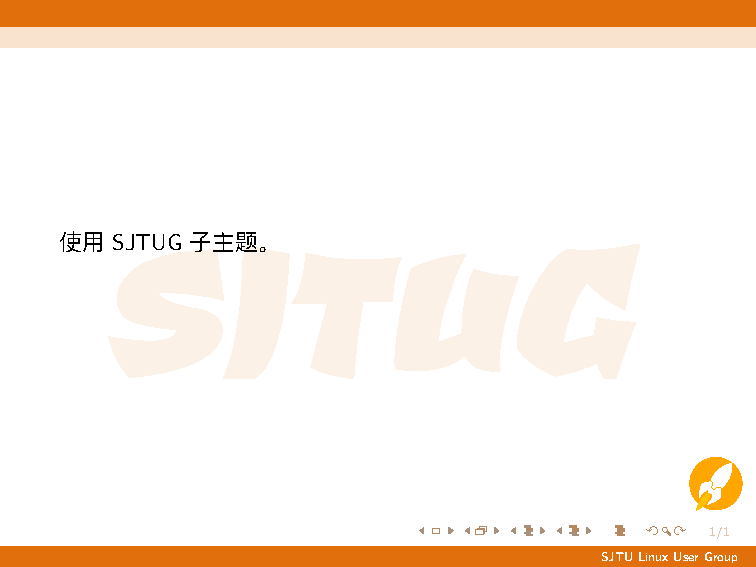
\includegraphics[width=|\only<1-3>{4cm}\only<4->{0.4\textbackslash{}textwidth}|]{sjtug}
|\highlightline<7>|  \caption{SJTUG 徽标}\label{fig:sjtug}
|\highlightline<5>|\end{figure}
\end{document}
      \end{codeblock}
    \end{column}
    \begin{column}{0.4\textwidth}
      \only<1>{
        \includepdflarge{support/examples/insertimage.pdf}
      }

      \only<2>{
        为了插入外部图片,需要使用 \pkg{graphicx} 宏包。之后在文档主体便可以使用 \cmd{includegraphics} 插入图片。导言区也可以加入 \cmd{graphicspath} 指定图片文件夹\footnotemark。
      }

      \only<3>{
        \cmd{includegraphics} 命令便以相对路径的方式插入图片,如果无同名图片,那么后缀名可以省略。可以使用可选参数指定插入的图片尺寸,最佳实践是使用 \cmd{textwidth} 或 \cmd{linewidth} 的相对值指定尺寸大小,以在未来可能的布局更改中保留一定的灵活性。
        \note{比如我未来想变更为幻灯片的时候。}
      }

      \only<4>{
        也可以通过键值对的方法设置图片的其他属性。
        \note{事实上,\LaTeX{} 很多命令都是使用方括号添加可选参数的。}
        \begin{center}
          \footnotesize
          \begin{tabular}{rl}
            \opt{width} & 宽度 \\
            \opt{height} & 高度 \\
            \opt{scale} & 缩放 \\
            \opt{angle} & 角度 \\
          \end{tabular}
        \end{center}
      }

      \only<5>{
        \env{figure} 为一个浮动体环境(\env{table} 也是),可以将其移动到其他位置上以减少行文中的空白。可以添加可选参数以指定如何放置浮动体,最多可以使用四种位置描述符:
        \begin{center}
          \footnotesize
          \begin{tabular}{cll}
            \opt{h} & Here & 尽可能在这里 \\
            \opt{t} & Top & 页面顶部 \\
            \opt{b} & Bottom & 页面底部 \\
            \opt{p} & Page & 浮动体专页 \\
          \end{tabular}
        \end{center}
        还可以只使用 \pkg{float} 宏包提供的 \opt{H} 描述符以强制置于此处。
      }

      \only<6>{
        采用 \cmd{centering} 命令而不是 \env{center} 环境来水平居中图片。这将避免多余的纵向间距。
      }

      \only<7>{
        使用 \cmd{caption} 命令输入题注,如果这个命令写在插入图片前面,题注将会在上方(中文中一般对 \env{table} 环境这么做)。后面将会看到如何对留有标记(\cmd{label})的图片进行引用。
      }
    \end{column}
  \end{columns}
  \only<2>{\footnotetext{其命令参数每个为一个以 \texttt{/} 结尾的文件夹,每个文件夹需要使用大括号包裹起来。}}
\end{frame}

\begin{frame}[fragile]
  \begin{columns}
    \begin{column}{0.6\textwidth}
      \begin{codeblock}[]{插入双图}
\documentclass{ctexart}
\usepackage{graphicx}
\graphicspath{{figs/}{pics/}}
\begin{document}
  \begin{figure}[ht]
|\highlightline<1>|    \begin{minipage}{0.48\textwidth}
      \centering
      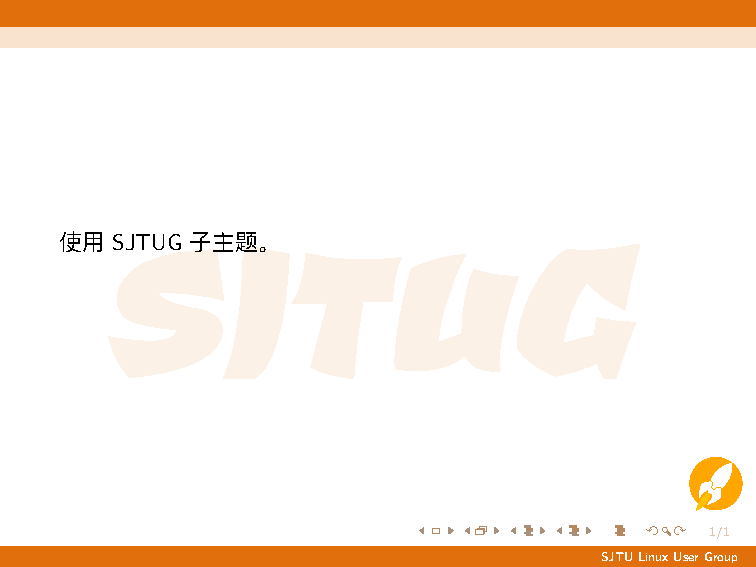
\includegraphics[height=2cm]{sjtug}
|\highlightline<2>|      \caption{SJTUG 徽标}\label{fig:sjtug}
|\highlightline<1>|    \end{minipage}\hfill
|\highlightline<1>|    \begin{minipage}{0.48\textwidth}
      \centering
      
\includegraphics[height=2cm]{sjtugt}
|\highlightline<2>|      \caption{SJTUG|\phantom{}|文字}\label{fig:sjtugt}
|\highlightline<1>|    \end{minipage}
  \end{figure}
\end{document}
      \end{codeblock}
    \end{column}
    \begin{column}{0.4\textwidth}

      \only<1>{
        在 \env{figure} 环境里使用 \env{minipage} 小页制作列盒子,以并排两图并分别编号,需要设定强制参数以指定列宽。两个小页之间添加 \cmd{hfill} 使两个小页两端对齐。
      }

      \only<2>{
        在每个小页内部分别使用 \cmd{caption} 添加标签。
      }

      \only<3>{
        \includepdflarge{support/examples/doubleimages.pdf}
      }
    \end{column}
  \end{columns}
\end{frame}

\begin{frame}[fragile]%
  \begin{columns}
    \begin{column}{0.6\textwidth}
      \begin{codeblock}[]{}
\documentclass{ctexart}
\usepackage{graphicx}
|\highlightline|\usepackage{subcaption}
\graphicspath{{figs/}{pics/}}
\begin{document}
  \begin{figure}[ht]
|\highlightline|    \begin{subfigure}{0.48\textwidth}
      \centering
      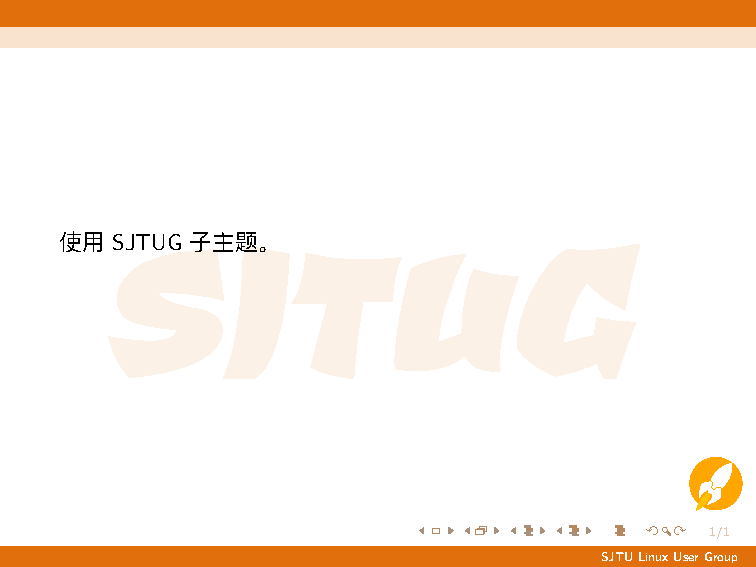
\includegraphics[height=2cm]{sjtug}
      \caption{|\phantom{}|徽标}
|\highlightline|    \end{subfigure}\hfill
|\highlightline|    \begin{subfigure}{0.48\textwidth}
      \centering
      
\includegraphics[height=2cm]{sjtugt}
      \caption{|\phantom{}|文字}
|\highlightline|    \end{subfigure}
    \caption{SJTUG}\label{fig:sjtug}
  \end{figure}
\end{document}
      \end{codeblock}
    \end{column}
    \begin{column}{0.4\textwidth}
      \includepdflarge{support/examples/subfigures.pdf}\vspace{15pt}
      \pkg{subcaption} 宏包提供了 \env{subfigure} 环境(以及 \env{subtable}),可以用于以子图的形式插入,编号会增加一级。也可以为子图添加子级引用编号。
    \end{column}
  \end{columns}
\end{frame}

\section{表}
\begin{frame}[fragile]
  \frametitle{简单表格}
  \begin{columns}
    \begin{column}{0.6\textwidth}
      \begin{codeblock}[]{}
\documentclass{ctexart}
|\only<1-2>{\highlightline}|\usepackage{|\temporal<1>{array}{\highlight{array}}{array},\temporal<2>{booktabs}{\highlight{booktabs}}{booktabs}|}
\begin{document}
\begin{table}[ht]
  \centering
  \caption{|\phantom{}|北京冬奥会吉祥物}
|\highlightline<1>|  \begin{tabular}{lp{3cm}}
|\highlightline<2>|    \toprule
|\highlightline<3>|吉祥物 & 描述                          \\
|\highlightline<2>|    \midrule
|\highlightline<3>|冰墩墩 & 2022 年北京冬季奥运会吉祥物  \\
|\highlightline<3>|雪容融 & 2022 年北京冬季残奥会吉祥物  \\
|\highlightline<2>|    \bottomrule
|\highlightline<1>|  \end{tabular}
\end{table}
\end{document}
      \end{codeblock}
    \end{column}
    \begin{column}{0.4\textwidth}
      
      \only<1>{
        使用 \env{tabular} 环境绘制表格。需要添加参数(称为\textbf{表格导言})以确定每一列的对齐方式。引入 \pkg{array} 宏包来使用更多的\textbf{引导符}。
        \begin{center}
          \footnotesize
          \begin{tabular}{>{\ttfamily}ll}
            \alert{l} & 向左对齐 \\
            \alert{c} & 居中对齐 \\
            \alert{r} & 向右对齐 \\
            \alert{p\{3cm\}} & 固定列宽,两端对齐 \\
            \alert{m\{3cm\}} & \texttt{p} + 垂直居中对齐 \\
            \alert{>\{\textbackslash{}bfseries\}} & 后一列单元格前加命令 \\
            \alert{*\{3\}\{l\}} & 三个左对齐列 \\
          \end{tabular}
        \end{center}
      }

      \only<2>{
        \pkg{booktabs} 宏包提供了标准三线表格所需要的行分割线:\cmd{toprule},\cmd{midrule},\cmd{bottomrule}。也可以使用 \cmd{cmidrule\{1-2\}} 来部分地绘制行分割线。一般不推荐在专业表格中使用纵向分割线。
      }

      \only<3>{
        每行内容使用 \textbackslash\textbackslash{} 分隔开,每行中的单元格使用 \& 分隔开。
      }

      \only<4>{
        \includepdflarge{support/examples/table.pdf}
      }
    \end{column}
  \end{columns}
\end{frame}

\begin{frame}[fragile]%
  \begin{columns}
    \begin{column}{0.6\textwidth}
      \begin{codeblock}[]{表头居中}
\documentclass{ctexart}
\usepackage{array,booktabs}
\begin{document}
\begin{table}[ht]
  \centering
  \caption{|\phantom{}|北京冬奥会吉祥物}
  \begin{tabular}{lp{3cm}}
    \toprule
|\highlightline|\multicolumn{1}{c}{|\phantom{}|吉祥物} &
|\highlightline|\multicolumn{1}{c}{|\phantom{}|描述} \\
    \midrule
|\phantom{}|冰墩墩 & 2022 年北京冬季奥运会吉祥物  \\
|\phantom{}|雪容融 & 2022 年北京冬季残奥会吉祥物  \\
    \bottomrule
  \end{tabular}
\end{table}
\end{document}
      \end{codeblock}
    \end{column}
    \begin{column}{0.4\textwidth}
      \cmd{multicolumn} 命令不仅可以用于合并同行的单元格,还可以用于临时地屏蔽表格导言对该列的对齐方式定义。这里用于居中表头。
      \begin{center}
        \parbox{0.85\linewidth}{
          \cmd{multicolumn\{格数\}\{对齐方式\}\{内容\}}
        }
      \end{center}
      跨页表格考虑使用 \pkg{longtable} 宏包。带标注的表格可以考虑使用 \pkg{threeparttable} 宏包。考虑使用在线工具生成表格代码 \link{https://www.tablesgenerator.com/latex_tables}。
      \note{复杂的使用方法在 \SJTUThesis{} 示例文档中都有提及。}
    \end{column}
  \end{columns}
\end{frame}

\section{数学公式}
\begin{frame}
  \frametitle{数学模式}
  \begin{alertblock}{}
  输入数学公式是 \LaTeX{} 的绝对强项,很多常见的公式服务依赖于一些轻量级渲染引擎比如 MathJax, K\kern-.3ex\raise.4ex\hbox{\footnotesize A}\kern-.3ex\TeX{}。但是它们实际上使用的是 \LaTeX{} 语法变种,也就是说并没有使用 \LaTeX{} 后端。所以不要期望有完全一致的输出。
  \end{alertblock}
  
  为了更好的获得数学公式输入支持,请使用 \hologo{AmS}math 宏包。数学模式分为两种:
  \begin{description}
    \item[行内模式] 一般通过一对美元符号(\$$\cdots$\$)标记,可以使用编辑器内建的符号表输入数学符号,也可以使用在线工具手写识别 \link{https://detexify.kirelabs.org/classify.html}。
    \item[行间模式] 一般通过 \env{equation} 环境\footnote{这是有编号环境,其加星号的变种 \env{equation*} 用于生成无编号环境。}输入。如果需要使用多行公式,请使用 \env{align} 环境,并按照类似表格输入的方式,使用 \& 对齐符号,\textbackslash\textbackslash{} 换行。如果不想手动居中,可以考虑多行自动居中的 \env{gather} 和单个大型公式首尾两端对齐 \env{multline}。
  \end{description}
  \note{关于表格和数学公式,如果不太熟悉如何输入,或者符号表记不住,推荐从比较容易上手的编辑器起步,比如 \TeX{}studio 提供了用户友好的界面(\faWindows{} 上的向导 $\rightarrow$ 数学助手)。我相信输入半年后,就可以对这些符号的输入很熟练了。
  
  你会发现我的这套教程没有讲很多的数学公式输入技巧,因为这些东西只有你自己熟练了才能体会。而且 \LaTeX{} 本来就不是完全关于数学公式的。}
\end{frame}

\begin{frame}
  \frametitle{数学命令展示}
  \begin{columns}
    \begin{column}{0.33\textwidth}
      \begin{exampleblock}{}
        $PV=nRT$
      \end{exampleblock}
      \begin{exampleblock}{}
        $\sum_{i=1}^ki^2=\frac{n(n+1)(2n+1)}{6}$
      \end{exampleblock}
      \begin{exampleblock}{}
        $T(n) = aT\left(\left\lceil\frac{n}{b}\right\rceil\right) + \mathcal{O}(n^d)$
      \end{exampleblock}
      \begin{exampleblock}{}
        $\frac{x_{1}+x_{2}+x_{3}}{3}\geq \sqrt[3]{x_{1}x_{2}x_{3}}$
      \end{exampleblock}
      \begin{exampleblock}{}
        $n=(\underbrace{1\cdots 1}_{k\text{ of 1's}})_2=2^{k+1}-1$
      \end{exampleblock}
      \begin{exampleblock}{}
        $\nabla f (P)= \left.\left(\frac{\partial f}{\partial x},\frac{\partial f}{\partial y},\frac{\partial f}{\partial z}\right)\right|_{P}$
      \end{exampleblock}
    \end{column}
    \begin{column}{0.67\textwidth}
      \begin{exampleblock}{}
        \begin{equation*}
          \int_{a}^b f(x)\,\mathrm{d}x=\lim_{|P|\rightarrow 0}\sum_{i=1}^n f(\xi_i)\Delta x_i
        \end{equation*}
      \end{exampleblock}
      \begin{exampleblock}{}
        \begin{equation}
          T(n) = \begin{cases}
            \mathcal{O}(n^d),&\textrm{if } d>\log_b a, \\
            \mathcal{O}(n^d\log n), &\textrm{if } d=\log_b a,\\
            \mathcal{O}(n^{\log_b a}), &\textrm{if } d<\log_b a.
          \end{cases}
        \end{equation}
      \end{exampleblock}
      \begin{exampleblock}{}
        \begin{align}
          Q^{T}A&=R \\
          \begin{pmatrix}
            q_1^T \\ q_2^T \\ q_3^T
          \end{pmatrix}
          \begin{pmatrix}
            a_1 & a_2 & a_3
          \end{pmatrix}
          &=R
        \end{align}
      \end{exampleblock}
    \end{column}
  \end{columns}
  \note{关于如果 \LaTeX{} 报出了错误,比如说数学模式下不能有空行,想要学习如何修复这些错误,
  可以详见 Learn\LaTeX{}.org 的相关章节
  \link{https://github.com/CTeX-org/learnlatex.github.io/blob/zh-Hans/zh-Hans/lesson-15.md}。}
\end{frame}

%更深入地讲解 mathtools, unicode-math, siunix

\section{引用}
\begin{frame}[fragile]
  \frametitle{交叉引用}
  \only<1>{
    正如之前所提到的,\LaTeX{} 中使用 \cmd{label} 标记,然后可以使用 \cmd{ref} 来引用这个标记。 \cmd{label} 可以放在使用计数器的对象之后。
  }

  \only<2>{
    为了使得对公式编号的引用带有括号,推荐使用 \hologo{AmS}math 宏包中的 \cmd{eqref} 命令。对于多行公式环境,每一个换行符前都可以添加一个 \cmd{label} 用于引用该行公式。
  }
  
  \begin{columns}
    \begin{column}{0.5\textwidth}
      \begin{codeblock}[]{图}
\begin{figure}
|\highlightline<1>|  \caption{|\phantom{}|示例}\label{fig:example}
\end{figure}
      \end{codeblock}
      \begin{codeblock}[]{表}
\begin{table}
|\highlightline<1>|  \caption{|\phantom{}|示例}\label{tab:example}
\end{table}
      \end{codeblock}
    \end{column}
    \begin{column}{0.5\textwidth}
\begin{codeblock}[]{目次}
|\highlightline<1>|\section{|\phantom{}|示例}\label{sec:example}
\end{codeblock}

\begin{codeblock}[]{公式}
\begin{equation}
  a = b + c
|\highlightline<1>|\label{eq:example}
\end{equation}
|\highlightline<2>|如公式 \eqref{eq:example} 所示,
\end{codeblock}
    \end{column}
  \end{columns}
\end{frame}

\begin{frame}[fragile]
  \frametitle{文献引用}
  \LaTeX{} 可以通过专用数据库文件 \texttt{.bib} 自动生成参考文献,很多的文献管理文件比如 EndNote \link{https://lic.sjtu.edu.cn/Default/softshow/tag/MDAwMDAwMDAwMLGImKE}, Zotero \link{https://www.zotero.org/}, JabRef \link{https://www.jabref.org/} 都可以直接导出这种格式的文件用于 \LaTeX{} 论文中的引用。一般不需要手写数据库文件,你只需要注意每一个文献会在数据库中有一个主键,这个类似于上文的 \cmd{label} 标记,只是要引用数据库中的文献需要使用 \cmd{cite} 命令。
  
  \begin{codeblock}[]{ref.bib}
|\highlightline|@article{devoftech,|\hfill\alert{\% 类型为期刊论文,主键为\texttt{devoftech}}|
  title={|\phantom{}|新时期我国信息技术产业的发展},
  author={|\phantom{}|江泽民},
  year={2008}
}
  \end{codeblock}
\end{frame}

\begin{frame}
  \frametitle{文献引用}
  而让 \LaTeX{} 处理 \texttt{.bib} 数据库文件与引用有两种工作流。你可能需要查清楚如何在编辑器中设置对应的工作流,或者采用后面所提到的高级编译方式 \texttt{latexmk}。
  \begin{columns}
    \begin{column}{0.5\textwidth}
      \begin{block}{\hologo{BibTeX} + \pkg{natbib}}
        一般期刊提交使用这种方法,\pkg{natbib} 宏包将提供命令 \cmd{citet}(文本引用) 和 \cmd{citep}(括号引用)。
      \end{block}
      \begin{alertblock}{\hologo{BibTeX} + \pkg{gbt7714}}
        中文引用可以直接使用 \pkg{gbt7714} 宏包,但是角模式和正文模式不能混用。
      \end{alertblock}
    \end{column}
    \begin{column}{0.5\textwidth}
      \begin{block}{\hologo{biber} + \pkg{biblatex}}
        这是更容易自定义的方法,与 \hologo{BibTeX} 的运作方式稍有不同。\pkg{biblatex} 提供了更加智能的引用命令。
      \end{block}
      \begin{alertblock}{\hologo{biber} + \pkg{biblatex-gb7714-2015}}
        而中文引用可以使用 \pkg{biblatex} 宏包的样式 \pkg{gb7714-2015}。
      \end{alertblock}
    \end{column}
  \end{columns}
\end{frame}

\begin{frame}[fragile]
  \frametitle{文献引用}
  \begin{columns}
    \begin{column}{0.5\textwidth}
      \begin{codeblock}[]{\hologo{BibTeX} + \pkg{gbt7714}}
\documentclass{ctexart}
\usepackage{gbt7714}
\bibliographystyle{gbt7714-numerial}
% \citestyle{numbers}  % 正文模式
\begin{document}
  |\phantom{}|他指出了...\cite{devoftech}
  \bibliography{ref}
\end{document}
      \end{codeblock}
    \end{column}
    \begin{column}{0.5\textwidth}
      \begin{codeblock}[]{\hologo{biber} + \pkg{biblatex-gb7714-2015}}
\documentclass{ctexart}
\usepackage[backend=biber,style=gb7714-2015]{biblatex}
\addbibresource{ref.bib}
\begin{document}
  |\phantom{}|他在文献 \parencite{devoftech}
  |\phantom{}|指出了...\cite{devoftech}
  \printbibliography
\end{document}
      \end{codeblock}
    \end{column}
  \end{columns}
\end{frame}

\begin{frame}
  \frametitle{文献引用}
  \begin{columns}
    \begin{column}{0.5\textwidth}
      \includepdflarge{support/examples/bibtex.pdf}
    \end{column}
    \begin{column}{0.5\textwidth}
      \includepdflarge{support/examples/biblatex.pdf}
    \end{column}
  \end{columns}
  \note{这页有一篇上过《新闻联播》的论文。}
\end{frame}

\end{shadedsection}

|\highlightline<3>|  % !TeX root = ../../latex-talk.tex

\part{SJTUThesis}

\begin{frame}
  \frametitle{本部分主要参考}
  \begin{bibliolist}{00}
    \onlineitem \textsc{SJTUG}.
    \newblock \textsc{SJTUThesis} 示例文档[EB/OL].
    \newblock 2022. \url{https://github.com/sjtug/SJTUThesis}.

    \onlineitem \textsc{SJTUG}.
    \newblock \textsc{SJTUThesis} 用户文档[EB/OL].
    \newblock 2022. \url{https://github.com/sjtug/SJTUTeX}.
  \end{bibliolist}
\end{frame}

\begin{frame}
  \frametitle{简介}
  \begin{columns}
    \begin{column}{0.6\textwidth}
      \begin{itemize}
        \item 最早由韦建文于 2009 年 11 月发布 0.1a 版
        \item 2018 年起由 SJTUG 接手维护
        \item 2019 年 6 月吴伟健重构了整个宏包的代码,升级版本号为 1.0
        \item 2022 年 11 月模板改版后,吴伟健、张驰等人使用 \LaTeX3 重构 2.0 版本
        \item 最新版:\SJTUThesisVersion{} (\SJTUThesisDate)
        \item 支持本科、硕士、博士学位论文的排版
        \item 推荐使用最新版本的 \TeX{} 发行版编译
      \end{itemize}
    \end{column}
    \begin{column}{0.4\textwidth}
      \begin{exampleblock}{}
        \begin{minipage}[c]{1cm}
          \includegraphics[width=0.8cm]{\getcontribpath{sjtug}{vi/sjtug}}
        \end{minipage}
        \begin{minipage}[c]{3cm}
          \href{https://github.com/sjtug}{sjtug}/\href{https://github.com/sjtug/SJTUThesis}{SJTUThesis}
        \end{minipage}
      \end{exampleblock}
      \vspace{-8pt}
      \begin{block}{}
        \scriptsize
        上海交通大学 \hologo{XeLaTeX} 学位论文及课程论文模板 | Shanghai Jiao Tong University \hologo{XeLaTeX} Thesis Template
      \end{block}
      \vspace{-8pt}
      \begin{alertblock}{}
        \scriptsize
        \begin{tabular}{cl}
          \faStar & 2.6k \\
          \faEye & 52 \\
          \faCodeBranch & 726 \\
        \end{tabular}
      \end{alertblock}
    \end{column}
  \end{columns}
\end{frame}

\begin{frame}
  \frametitle{\only<1>{为什么使用 \LaTeX{} 排版论文?}\only<2>{当然它们也互相学习}}
  \begin{columns}[t]
    \begin{column}{0.25\textwidth}
      \begin{exampleblock}{\faMarkdown{} Markdown}
        \begin{itemize}
          \item[\faPlus] 技术文档流行
          \item[\faPlus] 语法简单 
          \item[\faMinus] 不内置格式控制
        \end{itemize}
      \end{exampleblock}
      \only<2>{
        \begin{block}{}
          \begin{itemize}
            \item[\faBolt] R Markdown (Bookdown) 模板 \link{https://github.com/bubifengyun/SJTUThesis-Rmd} \link{https://github.com/bubifengyun/SJTUThesis-Rmd}
            \item[\faAsterisk] 配套 MathJax 渲染公式  
          \end{itemize}
        \end{block}
      }
    \end{column}
    \begin{column}{0.25\textwidth}
      \begin{exampleblock}{\faFileWord{} Word}
        \begin{itemize}
          \item[\faPlus] 通用论文格式
          \item[\faPlus] 所见即所得
          \item[\faMinus] 进阶排版仍困难 
        \end{itemize}
      \end{exampleblock}
      \only<2>{
        \begin{block}{}
          \begin{itemize}
            \item[\faBolt] 数学公式可以直接通过 \LaTeX{} 格式转换
            \item[\faAsterisk] 也就是 Unicode Math 输入方式 
          \end{itemize}
        \end{block}
      }
    \end{column}
    \begin{column}{0.25\textwidth}
      \begin{block}{\LaTeX{} SJTUThesis}
        \begin{itemize}
          \item[\faPlus] 学术论文格式
          \item[\faPlus] 内容样式分离
          \item[\faMinus] 上手有门槛 
        \end{itemize}
      \end{block}
      \only<2>{
        \begin{exampleblock}{}
          \begin{itemize}
            \item[\faBolt] \TeX{} 的可视前端 \hologo{LyX} \link{https://www.lyx.org/Download} Overleaf Rich Text 模式
            \item[\faAsterisk] \TeX{} 的可视改良 \TeX{}\raise-0.25em\hbox{\footnotesize MACS} \link{http://texmacs.org/tmweb/home/welcome.en.html} \link{https://mogan.app}
          \end{itemize}
        \end{exampleblock}
      }
    \end{column}
    \begin{column}{0.25\textwidth}
      \begin{exampleblock}{\faAdobe{} InDesign}
        \begin{itemize}
          \item[\faPlus] 专业杂志排版
          \item[\faPlus] 精细调整
          \item[\faMinus] 过于繁琐专业  
        \end{itemize}
      \end{exampleblock}
      \only<2>{
        \begin{block}{}
          \begin{itemize}
            \item[\faBolt] 传说用了 \TeX{} 的一些算法 \link{https://mp.weixin.qq.com/s/GASGHK-GsIg2Fwb2jWwpvw}
          \end{itemize}
        \end{block}
      }
    \end{column}
  \end{columns}
  \note{\emph{这页仅作简要介绍。}

  让我们来讨论 the elephant in the room:为什么用 \LaTeX{} 排版论文?
  }
  \note<1>[item]{Markdown 很好啊,方便的语法,一般技术文档也常用。但就是因为它太简单了,没有内置样式控制,一般需要借助 HTML,CSS 那一套东西。}
  \note<2>[item]{也会有一些人尝试通过 R Markdown(Bookdown)改进,当然你也可以试着使用 \LaTeX{} 里的 \pkg{markdown} 宏包
  (这有点像各种前端博客框架渲染 Markdown 为 HTML,只不过这里渲染 \LaTeX{} 生成 PDF,代码抄录方面已经有 Sphinx 这个工具 \link{https://github.com/sphinx-doc/sphinx}),
  以及可以通过 MathJax 渲染 \TeX{} 公式。
  }
  \note<1>[item]{Word 很好啊,官方钦定的论文写作方法,可见即可得,但是进阶排版仍然可以困难。就拿排版公式来说,
  大家以前初高中学的、或者是计算机二级考的 Word 2003 要排版公式,一种是装 MathType 插件,版本间不兼容、一种是搞个域代码+替换字体。}
  \note<2>[item]{Word 2007 之后添加了插入正经的 Unicode 公式功能,但默认的 Calibri Math 字体以及符号布局仍然赶不上 \TeX{} 的美感。
  }
  \note<1>[item]{根据之前学到的一些技巧,看起来不难对吧(虽然有我诱导的成分),然后它内容与样式分离的设计理念已经渗入了很多领域。以及很多学术论文都需要 \LaTeX{} 的提交。}
  \note<2>[item]{当然现在也推出了可见即可得的编辑器 \hologo{LyX},Overelaf 的可视模式(虽然这两个并不是一个东西);以及迟先生很喜欢的 TeXmacs,一种不使用 \TeX{} 底层的、但是效果相像的排版程序。
  }
  \note<1>[item]{设计相关专业的同学可能更喜欢 Adobe Indesign,对图文混排更为擅长。但是它也足够复杂,虽然提供了几乎所有的排版用具,但是我还没见过用它排版几十页充满公式的论文的(或许有人会开先河?)。}
  \note<2>[item]{以及传说它用了 \TeX{} 的一些算法,所以 \TeX{} 还是老大哥,兼具美感和批量化处理的折中方法。}
\end{frame}

\begin{frame}
  \frametitle{开始使用}
  \alert{下载} 推荐安装 Git \link{https://git-scm.com/} 后,克隆 SJTUG 镜像仓库
  \begin{exampleblock}{\faGit*}
    \ttfamily\small
    git clone https://mirror.sjtu.edu.cn/git/SJTUThesis.git/
  \end{exampleblock}

  \alert{编译} 推荐使用 \pkg{latexmk} 编译\footnote{\hologo{MiKTeX} 用户需要手动安装 Perl 解释器 \link{https://www.perl.org/get.html} 才能使用 \pkg{latexmk}。},在不能够利用自带的 \texttt{.latexmkrc} 配置文件的情况下,需要查清楚在对应的编辑器中如何使用 \hologo{XeLaTeX} + \hologo{biber} 编译\footnote{这种情况下,你可能需要查清楚如何全局安装该文档类,并刷新文件名数据库。} \link{https://github.com/sjtug/SJTUThesis/blob/master/README.md}。
  \begin{exampleblock}{\faTerminal}
    \ttfamily\small
    latexmk -xelatex main
  \end{exampleblock}

  \alert{在线} 直接使用 Overleaf 链接 \link{https://www.overleaf.com/latex/templates/sjtuthesis-latex-thesis-template-for-shanghai-jiao-tong-university/mkdwbyjbtfgg?r=sdkbtJ4qGS8kDZQQ&rm=d&rs=b}。
  其他在线平台用户可以下载压缩包,上传至对应平台并采用 \hologo{XeLaTeX} 编译,请注意使用最新版本的 \TeX{} Live。
  \note{不会 Git 的同学可以直接 Download ZIP。}
\end{frame}

\begin{frame}
  \frametitle{手动编译}
  \alert{第一次编译失败} 如果没有办法通过通常方式编译成功,请尝试使用文件夹内附带 \faLinux{}\,\faApple{} \texttt{Makefile} 和 \faWindows{} \texttt{Compile.bat} 进行编译。

  \alert{统计字数} 编写过程中也可以使用对应的命令调用 \TeX{}count 来统计正文字数。
  \begin{columns}
    \begin{column}{0.38\textwidth}
      \begin{exampleblock}{\faLinux{}\,\faApple}
        \ttfamily
        make all\\
        make clean\\
        make cleanall\\
        make wordcount
      \end{exampleblock}
    \end{column}
    \begin{column}{0.38\textwidth}
      \begin{exampleblock}{\faWindows}
        \ttfamily
        ./Compile.bat thesis\\
        ./Compile.bat clean\\
        ./Compile.bat cleanall\\
        ./Compile.bat wordcount
      \end{exampleblock}
    \end{column}
    \begin{column}{0.24\textwidth}
      \begin{block}{\faInfo}
        \ttfamily
        编译论文\\
        清理中间文件\\
        $\hookrightarrow +$删除论文\\
        统计字数
      \end{block}
    \end{column}
  \end{columns}
\end{frame}

\begin{frame}[label=compile]
  \frametitle{编译问题排查}
  \begin{columns}
    \begin{column}{0.33\textwidth}
      \begin{alertblock}{无法使用 \texttt{latexmk}\thesisissue{578}}
        \hologo{MiKTeX} 需要安装 Perl 解释器。
      \end{alertblock}  
      \begin{alertblock}{\CTeX{} 套装无法编译\thesisissue{446}}
        使用最新 \TeX{} 发行版。\link{https://github.com/Aloft-Lab/CTeX-Installer}
      \end{alertblock}
      \begin{alertblock}{\hologo{pdfLaTeX} 无法编译\thesisissue{444}}
        请使用 \texttt{latexmk},或更改编辑器设置以 \hologo{XeLaTeX} 编译。
      \end{alertblock}
    \end{column}
    \begin{column}{0.33\textwidth}
      \begin{alertblock}{缺少字体\thesisissue{564} \thesisdiscuss{598}}
        更换字体集,或者安装对应字体。
      \end{alertblock}
      \begin{alertblock}{缺少汉字\thesisissue{533} \thesisdiscuss{617}}
        去除使用 fandol 字体集的设定。或者是安装字体后,改用 \texttt{cjk-font=adobe} 或 \texttt{cjk-font=founder}。
      \end{alertblock}
    \end{column}
    \begin{column}{0.33\textwidth}
      \begin{block}{\faInfoCircle{} README}
        不同编辑器的设置请首先参阅 README \link{https://github.com/sjtug/SJTUThesis/blob/master/README.md} 文档。
      \end{block}
      \begin{block}{\faBookOpen{} Wiki}
        其他编译问题推荐查阅 Wiki \link{https://github.com/sjtug/SJTUThesis/wiki} 的使用说明部分。
      \end{block}
    \end{column}
  \end{columns}
  \note{两个进阶问题:
  
  如果之前出现了编译错误,在重新编译前,最好清理一下临时文件(\texttt{make clean})。

  如果是 biber 出现了问题,还可以尝试 \texttt{rm -rfv \$(biber --cache)}。\thesisdiscuss{774}
  }
\end{frame}

\begin{frame}[label=covers]
  \frametitle{论文组成}
  \begin{figure}[h]
    \centering
    \foreach \thesispage/\thesisnote in {
      1/{中文封面},3/{英文封面},5/{版权页},7/{中文摘要},9/{英文摘要},11/{目录},13/{插图目录},15/{表格目录},
      17/{正文},27/{参考文献},29/{附录},31/{成果},33/{致谢},35/{大摘要}} {%
      \begin{subfigure}{.13\textwidth}
        \centering
        \fzerobox{\includegraphics[width=\textwidth,page=\thesispage]{support/thesis/sample-thesis-zh.pdf}}
        \caption{\thesisnote}
      \end{subfigure}
    }
  \end{figure}
  \note{虽然说符号表在新版中是要放在附录中,但是学位论文规范中却说可以放在正文前,所以你可以自行选择。}
  \note{文档中的彩色框是标识超链接,印刷时不会输出,如果希望关闭可以向 \pkg{hyperref} 宏包添加可选参数 \opt{hidelinks}。}
\end{frame}

\begin{frame}[fragile]
  \frametitle{文档类选项}
  \begin{columns}
    \begin{column}{0.35\textwidth}
      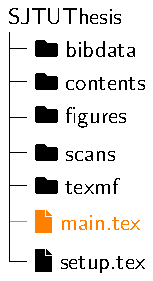
\includegraphics[page=1]{support/figures/thesisdir.pdf}
    \end{column}
    \begin{column}{0.65\textwidth}
      文档类选项是指在载入文档类时的可选选项,多个选项使用逗号隔开,文档类选项会对所有宏包可见。
      \begin{codeblock}[escapechar="]{main.tex}
% !TeX encoding = UTF-8

% 载入 SJTUThesis 模版
"\highlightline"\documentclass[type=master]{sjtuthesis}
% 选项
%   type=[doctor|master|bachelor],
%   zihao=[-4|5],
%   lang=[zh|en],
%   review,
%   [twoside|oneside],
%   math-style=[ISO|TeX],
      \end{codeblock}
    \end{column}
  \end{columns}
\end{frame}

\begin{frame}[fragile]
  \frametitle{文档类选项}
  \begin{columns}
    \begin{column}{0.3\textwidth}
      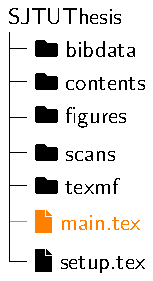
\includegraphics[page=1]{support/figures/thesisdir.pdf}
    \end{column}
    \begin{column}{0.7\textwidth}
      我是学士,写英文论文
      \begin{codeblock}[]{}
|\phantom{}|\documentclass[type=bachelor,lang=en]{sjtuthesis}
      \end{codeblock}
      我是硕士,盲审
      \begin{codeblock}[]{}
|\phantom{}|\documentclass[type=master,review]{sjtuthesis}
      \end{codeblock}
      我是博士,先写着电子版不空页
      \begin{codeblock}[]{}
|\phantom{}|\documentclass[type=doctor,oneside]{sjtuthesis}
      \end{codeblock}
    \end{column}
  \end{columns}
  \note{有 ChatGPT 那味了。}
\end{frame}

\begin{frame}
  \frametitle{文档类选项}
  \begin{columns}
    \begin{column}{0.35\textwidth}
      \includegraphics[page=2,scale=0.9]{support/figures/thesisdir.pdf}
    \end{column}
    \begin{column}{0.65\textwidth}
      \begin{table}
        \caption{文档类选项}
        \footnotesize
        \begin{tabular}{>{\ttfamily}rll}
          \toprule
          选项 & 含义 & 相关 \\
          \midrule
          type= & 指定论文类型 & 第 \ref{covers} 页\\
          \midrule
          cjk-font= & 指定中文字体 & \\
          text-font= & 指定西文字体 & 第 \ref{frame:fonts} 页\\
          math-font= & 指定数学字体 & \\
          math-style= & 指定数学样式 & 第 \ref{frame:math-style} 页\\
          \midrule
          review & 开启盲审模式 & \thesisissue{195} \thesisissue{686} \\
          twoside & 双页模式 & \thesisissue{554} \\
          oneside & 单页模式 & \thesisissue{694} \\
          openright & 章从奇数页开始 & \thesisdiscuss{724} \\
          openany & 章从任意页开始 & \thesisissue{446} \\
          \bottomrule
        \end{tabular}
      \end{table}

      更多文档类选项查阅 \textsc{SJTU\TeX{}} 的开发文档 \link{https://github.com/sjtug/SJTUTeX/releases/download/v1.1.0/sjtuthesis.pdf}。
    \end{column}
  \end{columns}
\end{frame}

\begin{frame}[label={frame:fonts}]
  \frametitle{字体配置}
  \newcommand{\noticemark}{\alert{\normalshape \textopenbullet}}
  \begin{columns}
    \begin{column}{0.35\textwidth}
      \includegraphics[page=3,scale=0.9]{support/figures/thesisdir.pdf}
    \end{column}
    \begin{column}{.65\textwidth}
      相较于 \CTeX{} 使用 \texttt{fontset} 设定中文字体集,
      \SJTUThesis{} 还提供了西文、数学字体集的设定\footnotemark。

      {
        \medskip
        \ttfamily\scriptsize
        \alert{cjk-font=...\hfill 中文字体}
        
        \stamphrule\medskip

        \foreach \sjtufontname/\sjtufontdesc in {adobe/{adobe \faAdobe\noticemark},{fandol}/{fandol \faLinux{} \noticemark},{founder},mac/{mac \faApple{} \noticemark},windows/{windows \faWindows},ubuntu/{ubuntu \noticemark}}{
          \begin{minipage}{2.2cm}
            \centering
            \includefontpreview{support/thesis/cjkfont-\sjtufontname.pdf}\\
            \raisebox{0.8ex}{\sjtufontdesc}
          \end{minipage}
        }

        \bigskip

        \alert{text-font=..., math-font=...\hfill 西文与数学字体}

        \stamphrule\medskip

        \foreach \sjtufontname/\sjtufontdesc in {{cambria}/{cambria \noticemark},{lm},{newcm}/{newcm \noticemark},{newpx},{newtx},{stixtwo}/{stixtwo \noticemark},{times},{xits}/{xits \noticemark}}{
          \begin{minipage}{2cm}
            \centering
            \includefontpreview{support/thesis/latinfont-\sjtufontname.pdf}\\
            \raisebox{0.8ex}{\sjtufontdesc}
          \end{minipage}
        }
      }
    \end{column}
  \end{columns}
  \footnotetext{\noticemark 表示无法使用 pdf\LaTeX{} 编译。}
\end{frame}

\begin{frame}[label={frame:math-style}]
  \frametitle{数学样式}
  \begin{columns}
    \begin{column}{0.35\textwidth}
      \includegraphics[page=2,scale=0.9]{support/figures/thesisdir.pdf}
    \end{column}
    \begin{column}{0.65\textwidth}
      新增数学样式 \texttt{math-style} 文档类选项,现在默认为 \texttt{ISO},
      如果更喜欢原始的 \TeX{} 数学样式,可以切换为 \texttt{TeX}。

      \begin{minipage}[c]{10em}
        \texttt{math-style=ISO}
      \end{minipage}
      \begin{minipage}[c]{5cm}
        \includemathstylepreview{support/thesis/mathstyle-ISO.pdf}
      \end{minipage}
       
      \begin{minipage}[c]{10em}
        \texttt{math-style=TeX}
      \end{minipage}
      \begin{minipage}[c]{5cm}
        \includemathstylepreview{support/thesis/mathstyle-TeX.pdf}
      \end{minipage}

      \begin{block}{}
        请注意在默认情况下(\texttt{math-style=ISO})应当使用 \cmd{increment} 而不是 \cmd{Delta} 表示有限增量。
      \end{block}
    \end{column}
  \end{columns}
\end{frame}

\begin{frame}[fragile]
  \frametitle{基本配置}
  \begin{columns}
    \begin{column}{0.35\textwidth}
      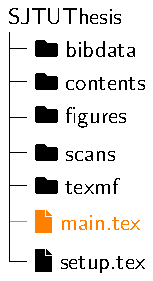
\includegraphics[page=1]{support/figures/thesisdir.pdf}
    \end{column}
    \begin{column}{0.65\textwidth}

      \only<1>{
        在 \texttt{main.tex} 中引入 \texttt{setup.tex} 来导入主要的信息录入与宏包加载配置。
      }

      \only<2>{
        \alert{\textbf{(a,b)}} 其中 \cmd{sjtusetup}(第 \ref{sjtusetup} 页)中的 \opt{info} 将会修改封面的信息设置。
      }

      \begin{codeblock}[firstnumber=12]{main.tex}
|\highlightline<1>|% 论文基本配置,加载宏包等全局配置
|\highlightline<1>|\input{setup}

\begin{document}

%TC:ignore

|\highlightline<2>|% 标题页
|\highlightline<2>|\maketitle
      \end{codeblock}
    \end{column}
  \end{columns}
\end{frame}

\begin{frame}[fragile, label=sjtusetup]
  \frametitle{基本配置}
  \begin{columns}
    \begin{column}{0.35\textwidth}
      \includegraphics[page=4]{support/figures/thesisdir.pdf}
    \end{column}
    \begin{column}{0.65\textwidth}
      \vspace*{-0.2cm}
      \begin{codeblock}[firstnumber=3]{setup.tex}
\sjtusetup{
  info = {
    zh/title  = {|\phantom{}|上海交通大学学位论文 \LaTeX{} 模板示例文档},
    en/title  = {A Sample for \LaTeX-based SJTU Thesis Template},
    zh/author = {|\phantom{}|某\quad{}某},
    en/author = {Mo Mo},
  },
  style = { float-seperator = {--}, },
  name = {
    achv = {|\phantom{}|攻读学位期间完成的论文},
  },
}
      \end{codeblock}
    \end{column}
  \end{columns}
\end{frame}

\begin{frame}[label=setup]
  \frametitle{基本配置}
  \begin{columns}
    \begin{column}{0.35\textwidth}
      \includegraphics[page=4]{support/figures/thesisdir.pdf}
    \end{column}
    \begin{column}{0.65\textwidth}
      \begin{table}
        \centering
        \caption{info 域}
        \footnotesize
        \begin{tabular}{lll} \toprule
          命令作用     & 中文对应选项                      & 英文对应选项                 \\ \midrule
          论文标题     & \texttt{zh/title}                 & \texttt{en/title}            \\
          关键字列表   & \texttt{zh/keywords}              & \texttt{en/keywords*}        \\
          作者姓名     & \texttt{zh/author}                & \texttt{en/author}           \\
          申请学位名称 & \texttt{zh/degree}                & \texttt{en/degree}           \\
          院系名称     & \texttt{zh/department}            & \texttt{en/department}       \\
          专业名称     & \texttt{zh/major}                 & \texttt{en/major}            \\
          导师         & \texttt{zh/supervisor}            & \texttt{en/supervisor}       \\
          副导师       & \texttt{zh/assoc-supervisor}      & \texttt{en/assoc-supervisor} \\
          联培导师     & \texttt{zh/co-supervisor}         & \texttt{en/co-supervisor}    \\
          日期         & \multicolumn{2}{c}{\texttt{date}}                                \\
          学号         & \multicolumn{2}{c}{\texttt{id}}                                  \\ \bottomrule
        \end{tabular}
      \end{table}
    \end{column}
  \end{columns}
  \note{有些选项是 v2 更名或新增的。}
  \note{注意现在使用语言前缀作为键名。}
\end{frame}

\begin{frame}[fragile]
  \frametitle{版权页}
  \begin{columns}
    \begin{column}{0.4\textwidth}
      \includegraphics[page=5]{support/figures/thesisdir.pdf}
    \end{column}
    \begin{column}{0.6\textwidth}
      \alert{\textbf{(c)}} \cmd{copyrightpage} 可以用于插入版权页。
      也可接受一个可选参数,用于直接使用扫描件,此时需要载入 \pkg{pdfpages} 包。\thesisissue{473}

      \begin{codeblock}[firstnumber=22]{main.tex}
% 原创性声明及使用授权书
\copyrightpage
% 插入外置原创性声明及使用授权书
% 导言区添加 \usepackage{pdfpages}
% \copyrightpage[scans/sample-copyright-old.pdf]
      \end{codeblock}
    \end{column}
  \end{columns}
\end{frame}

\begin{frame}[fragile]
  \frametitle{三个部分}
  \framesubtitle{前置部分}
  \begin{columns}
    \begin{column}{0.4\textwidth}
      \includegraphics[page=8]{support/figures/thesisdir.pdf}
    \end{column}
    \begin{column}{0.6\textwidth}
      \alert{\textbf{(d,e,f,g,h)}} 前言从 \cmd{frontmatter} 处开始,页码设置为大写罗马数字,主要包含摘要和目录内容。
      \begin{codeblock}[firstnumber=27]{main.tex}
|\highlightline|% 前置部分
|\highlightline|\frontmatter

% 摘要
\input{contents/abstract}

% 目录
\tableofcontents
% ...
      \end{codeblock}
    \end{column}
  \end{columns}
\end{frame}

\begin{frame}[fragile]
  \frametitle{三个部分}
  \framesubtitle{正文部分}
  \begin{columns}
    \begin{column}{0.4\textwidth}
      \includegraphics[page=9]{support/figures/thesisdir.pdf}
    \end{column}
    \begin{column}{0.6\textwidth}
      \alert{\textbf{(i,j,k)}} 正文从 \cmd{mainmatter} 处开始,页码设置为正常数字,包含正文、参考文献、附录内容。
      \begin{codeblock}[firstnumber=47]{main.tex}
|\highlightline|% 主体部分
|\highlightline|\mainmatter

% 正文内容
\input{contents/intro}
\input{contents/math_and_citations}
\input{contents/floats}
\input{contents/summary}

%TC:ignore

% 参考文献
\printbibliography[heading=bibintoc]

% 附录
\appendix
      \end{codeblock}
    \end{column}
  \end{columns}
\end{frame}

\begin{frame}[fragile]
  \frametitle{三个部分}
  \framesubtitle{结尾部分}
  \begin{columns}
    \begin{column}{0.4\textwidth}
      \includegraphics[page=10]{support/figures/thesisdir.pdf}
    \end{column}
    \begin{column}{0.6\textwidth}
      \alert{\textbf{(k,l,m,n)}} 结尾从 \cmd{backmatter} 处开始,页码设置为正常数字,包含致谢等相关情况。
      \begin{codeblock}[firstnumber=71]{main.tex}
|\highlightline|% 结尾部分
|\highlightline|\backmatter

% 用于盲审的论文需隐去致谢、发表论文、科研成果、简历

% 致谢
\input{contents/acknowledgements}

% 发表论文及科研成果
% 盲审论文中,发表论文及科研成果等仅以第几作者注明即可,不要出现作者或他人姓名
\input{contents/achievements}

%...
      \end{codeblock}
    \end{column}
  \end{columns}
\end{frame}

\begin{frame}
  \frametitle{数学定理环境}
  \begin{columns}
    \begin{column}{0.4\textwidth}
      \includegraphics[page=6]{support/figures/thesisdir.pdf}
    \end{column}
    \begin{column}{0.6\textwidth}
      \SJTUThesis{} 定义了常用的数学环境(需要引入 \pkg{ntheorem} 或者 \pkg{amsthm} 宏包)。

      \begin{table}
        \centering
        \caption{\textsc{SJTUThesis} 定义的数学环境}
        \footnotesize
        \begin{tabular}{>{\ttfamily}rl|>{\ttfamily}rl}
          \toprule
          assumption  & 假设  & lemma       & 引理 \\
          axiom       & 公理  & problem     & 问题 \\
          conjecture  & 猜想  & proof       & 证明 \\
          corollary   & 推论  & proposition & 命题 \\
          definition  & 定义  & remark      & 注   \\
          example     & 例    & solution    & 解   \\
          exercise    & 练习  & theorem     & 定理 \\
          \bottomrule
        \end{tabular}
      \end{table}
    \end{column}
  \end{columns}
\end{frame}

\begin{frame}[fragile]
  \frametitle{参考文献}
  \begin{columns}
    \begin{column}{0.4\textwidth}
      \includegraphics[page=7]{support/figures/thesisdir.pdf}
    \end{column}
    \begin{column}{0.6\textwidth}
      \begin{codeblock}[firstnumber=111,numbersep=2pt]{setup.tex}
% 使用 BibLaTeX 处理参考文献
%   biblatex-gb7714-2015 常用选项
%     gbnamefmt=lowercase     姓名大小写由输入信息确定
%     gbpub=false             禁用出版信息缺失处理
\usepackage[backend=biber,style=gb7714-2015]{biblatex}
% 文献表字体
% \renewcommand{\bibfont}{\zihao{-5}}
% 文献表条目间的间距
\setlength{\bibitemsep}{0pt}
|\highlightline|% 导入参考文献数据库
|\highlightline|\addbibresource{bibdata/thesis.bib}
      \end{codeblock}
    \end{column}
  \end{columns}
\end{frame}

\begin{frame}
  \frametitle{Word}
  \begin{itemize}
    \item[{\faQuestionCircle[regular]}] 跟 Word 的参考实现略有不同 
    \item[{\faCheckCircle[regular]}] 毕设论文的格式只要不违背《上海交通大学关于本科生毕业设计(论文)工作的指导意见》\link{https://github.com/sjtug/SJTUThesis/files/6505296/default.pdf} \thesisissue{621}、《上海交通大学博士、硕士学位论文撰写指南》\link{https://www.gs.sjtu.edu.cn/info/1143/5801.htm} \thesisissue{652} 即可,其他细节上的修改可以先搜索解决方案,再反馈给我们。
    \item[{\faQuestionCircle[regular]}] 我需要转为 Word 文档
    \item[{\faCheckCircle[regular]}] PDF 转为 Word 文档属于逆向工程,暂时不存在完全正确的转换方法 \link{https://www.bilibili.com/video/BV1Vi4y1C71M},从 \LaTeX{} 源代码出发的转换可以使用其他工具实现 \thesisissue{480} \thesisissue{500}。
  \end{itemize}
\end{frame}

\begin{frame}
  \frametitle{还有其他问题?}
  % \begin{columns}
    % \begin{column}{0.73\textwidth}
      \begin{itemize}
        \item[{\faComment*[regular]}] 日常模板或 \LaTeX{} 使用问题可以前往 Discussions \link{https://github.com/sjtug/SJTUThesis/discussions} 提问

        (解决后别忘了 \textcolor{green}{\faCheckCircle{} Mark as answer}
        \item[{\faDotCircle[regular]}] 如果是 \textsc{SJTUThesis} 项目本身的 bug 和 feature request

        可以通过 Issues \link{https://github.com/sjtug/SJTUThesis/issues} 反馈。
        \item[{\faCodeBranch}] 如果你有好点子,可以贡献代码

          向 \textsc{SJTU\TeX{}} \link{https://github.com/sjtug/SJTUTeX} 存储库发 PR,\par
          而后把解包结果同步到 \textsc{SJTUThesis}。
        
        \item[{\faQq}] 也欢迎在 QQ 群(715273806)即时讨论。
        \note{群之前满了,社长给腾讯充了钱,让它可以接着塞人。}
      \end{itemize}
    % \end{column}
    % \begin{column}{0.27\textwidth}
    %   
\includegraphics[height=0.7\textheight]{support/images/qq.jpg}
    % \end{column}
  % \end{columns}
\end{frame}

\end{document}
      \end{codeblock}
    \end{column}
  \end{columns}
  \note<3>{当然,如果需要不换页插入源代码就不用 \cmd{include} 了,
  因为这最主要的好处在于能够在组建大型文档的时候,得到当前页码、编号的进度信息。
  在插入小部件时,还是推荐使用 \cmd{input},这个命令不会额外地产生 \texttt{.aux} 文件,
  对于 I/O 反应慢的(说的就是 \faWindows{})比较友好。}
\end{frame}

\begin{frame}[fragile]
  \frametitle{组织文档}
  \begin{columns}
    \begin{column}{0.4\textwidth}
      \begin{codeblock}[]{learnlatex.tex}
|\highlightline|\chapter{|\phantom{}|学习 \LaTeX{}}
\section{|\phantom{}|概念}
\subsection{\LaTeX{}}
\LaTeX{} 是一个用以排版高质量作品的文档准备系统。
      \end{codeblock}
      子文件中就不需要添加 \env{document} 环境了\footnotemark。
    \end{column}
    \begin{column}{0.6\textwidth}
      \begin{codeblock}[]{主文档 main.tex}
|\highlightline|\documentclass{ctexrep}
\includeonly{learnlatex,sjtuthesis}
\begin{document}
  \tableofcontents
  % !TeX root = ../../latex-talk.tex

\part{学习 \LaTeX{}}
% FIXME: footnote fault numbering
% FIXME: section pop up in navigation in advance

\begin{frame}
  \frametitle{本部分主要参考}
  \begin{bibliolist}{00}
    \onlineitem 陈晟祺~等.
    \newblock 如何使用 \LaTeX\ 排版论文[EB/OL].
    \newblock 2021. \url{https://github.com/tuna/thulib-latex-talk}.

    \onlineitem 曾祥东.
    \newblock 现代 \LaTeX\ 入门讲座[EB/OL].
    \newblock 2022. \url{https://github.com/stone-zeng/latex-talk}.

    \onlineitem \LaTeX\ Project.
    \CTeX\ 开发小组~译.
    \newblock learnlatex.org[EB/OL].
    \newblock 2022. \url{https://github.com/CTeX-org/learnlatex.github.io}.
  
    \onlineitem \textsc{Oetiker T}, \textsc{Partl H}, \textsc{Hyna I}, \textsc{Schlegl E}.
    \CTeX\ 开发小组~译.
    \newblock 一份(不太)简短的 \LaTeXe{} 介绍:或 111 分钟了解 \LaTeXe{}[EB/OL]. \newblock\newblock 2021.
    \url{https://ctan.org/pkg/lshort-zh-cn}.
  \end{bibliolist}

  \note{推荐大家去阅读这些入门材料。}
\end{frame}

\begin{frame}[plain]
  \vfil
  \begin{center}
    \href{https://learnlatex.org}{
      \rmfamily
      Learn\,\lower1ex\hbox{\Huge\LaTeX{}}.org
    }
  \end{center}
  \vfil
  \begin{center}
    \parbox{0.75\linewidth}{
      Learn\LaTeX{}.org 提供了解 \LaTeX{} 的 16 篇简短的教程,并包含了一些可以在线运行的示例,可以通过亲自动手查看实验效果。本部分主要参考由 \CTeX{}-org 提供的中文翻译版本 \link{https://github.com/CTeX-org/learnlatex.github.io/tree/zh-Hans/zh-Hans/}。
    }
  \end{center}
  \vfil
  \note{这一部分主要参考了 Learn\LaTeX{}.org 的系列教程,内容简洁,适合入门,符合
  教育学观念 \link{https://www.tug.org/TUGboat/tb41-2/tb128reviews-learnlatex.pdf},
  并参考由 \CTeX{}-org 提供的中文翻译版本
  \link{https://github.com/CTeX-org/learnlatex.github.io/tree/zh-Hans/zh-Hans/}。
  如果你认为下面一个小时的入门教程没有讲得非常细致的话,
  欢迎直接阅读这个网站的全文。}
\end{frame}

\begin{shadedsection}

\section{是什么}
\begin{frame}
  \frametitle{\TeX{}}
  \begin{columns}[c]
    \begin{column}{0.7\textwidth}
      \begin{center}
        \rmfamily\Huge
        \hologo{La}\highlight[structure!70]{\TeX{}}
      \end{center}
      \begin{center}
        \parbox{0.75\textwidth}{
          \TeX{} 是由斯坦福大学教授高德纳
          (Donald E.~Knuth)于 1977 年开始开发的排版引擎。目前仍在更新,最新版本号为 3.141592653 \link{https://tug.org/TUGboat/tb42-1/tb130knuth-tuneup21.pdf}。
        }
      \end{center}
    \end{column}
    \begin{column}{0.3\textwidth}
      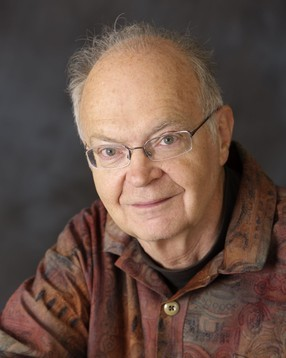
\includegraphics[width=.8\columnwidth]{support/images/Knuth.jpg}
    \end{column}
  \end{columns}
  \note{\emph{这一部分背景介绍大家可以了解一下,暂时跳过。}
  \LaTeX{} 这个词由两个部分组成,\hologo{La} 和 \TeX{}。那我们首先了解一下 \TeX{} 是什么。
  \TeX{} 是由斯坦福大学的教授高德纳于 1977 年开始开发的排版引擎,它已经有三十多年的历史了,
  目前仍在更新,版本号(3.141592653)将会趋近于 $\pi$ 的取值,高德纳最近还在给 \textsl{TUGBoat} 写稿子
  \link{https://tug.org/TUGboat/tb42-1/tb130knuth-tuneup21.pdf},
  关于 \TeX{} 今年又做了哪些改进。}
\end{frame}

\begin{frame}
  \frametitle{\LaTeX{}}
  \begin{columns}[c]
    \begin{column}{0.7\textwidth}
      \begin{center}
        \rmfamily\Huge
        \highlight[structure]{\LaTeX{}}
      \end{center}
      \begin{center}
        \parbox{0.75\textwidth}{
          \LaTeX{} 是最早在 1985 年由现就职于微软的 Leslie Lamport 开发的一种 \TeX{} \textbf{格式}\footnotemark,使用一些列宏和扩展宏包来简化 \TeX{} 的使用。现在由 \LaTeX{} Project 的成员维护。现在广泛使用的版本是 \LaTeXe{},最新的版本为 \LaTeX3(2020 年 10 月后默认内置)。
        }
      \end{center}
    \end{column}
    \begin{column}{0.3\textwidth}
      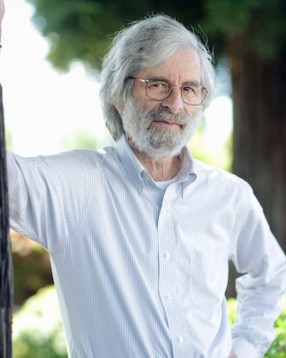
\includegraphics[width=.8\columnwidth]{support/images/Lamport.jpg}
    \end{column}
  \end{columns}
  \footnotetext{\hologo{ConTeXt} 也是一种 \TeX{} 格式 \link{https://www.contextgarden.net/}。}
  \note{\emph{这一部分的背景介绍大家可以了解一下,暂时跳过。}
  \LaTeX{} 是最早由现就职于微软的 Leslie Lamport 开发的一种 \TeX{} 格式(与其对标的是
  \hologo{ConTeXt}\link{https://www.contextgarden.net/}),主要也是为了简化 \TeX{} 的使用。
  现在主要由 \LaTeX{} 开发组维护,现在广泛使用的版本是 \LaTeXe{},最新的版本为 \LaTeX3,
  在 2020 年 10 月后默认内置,所以要尽可能使用较新的发行版,以充分发挥其功能。}
\end{frame}

\begin{frame}
  \frametitle{程序}
  \begin{columns}[c]
    \begin{column}{0.7\textwidth}
      \begin{center}
        \rmfamily\Huge
        \highlight[structure]{\hologo{pdfLaTeX}}
      \end{center}
      \begin{center}
        \parbox{0.7\textwidth}{
          \hologo{pdfLaTeX} 是为了编译一个 \LaTeX{} 文档而运行的程序。实际上底层在运行一个叫 \hologo{pdfTeX} 的引擎,并预装了对应的 \LaTeX{} \textbf{格式}。为了利用临时文件,可能就需要多次运行程序。
        }
      \end{center}
    \end{column}
    \begin{column}{0.3\textwidth}
      \begin{block}{}
        \ttfamily\small
        > \highlight{pdflatex} main.tex\\
        This is pdfTeX, Version 3.141592653-
        2.6-1.40.23 (MiKTeX 21.10)\\
        entering extended mode\\
        \highlight{LaTeX2e} <2021-11-15>\\
        \highlight{L3} programming layer <2021-11-22>
      \end{block}
    \end{column}
  \end{columns}
  \note{\hologo{pdfLaTeX} 是为了编译一个 \LaTeX{} 文档而运行的程序。}
\end{frame}

\begin{frame}
  \frametitle{引擎}
  \begin{columns}[c]
    \begin{column}{0.7\textwidth}
      \begin{center}
        \rmfamily\Huge
        \highlight[structure!70]{pdf}\hologo{La}\highlight[structure!70]{\TeX{}}
      \end{center}
      \begin{center}
        \parbox{0.7\textwidth}{
          pdf\TeX{} 是编译 \TeX{} 文档(以 \texttt{.tex} 结尾)的\textbf{引擎}---可以理解 \TeX{} 指令的\textbf{程序}。
        }
      \end{center}
    \end{column}
    \begin{column}{0.3\textwidth}
      \begin{block}{}
        \ttfamily\small
        > pdflatex main.tex\\
        This is \highlight[structure!70]{pdfTeX}, Version 3.141592653-
        2.6-1.40.23 (MiKTeX 21.10)
        entering extended mode\\
        LaTeX2e <2021-11-15>\\
        L3 programming layer <2021-11-22>
      \end{block}
    \end{column}
  \end{columns}
  \note{实际上底层在运行一个叫 \hologo{pdfTeX} 的引擎,并预装了对应的 \LaTeX{} 格式。}
\end{frame}

\begin{frame}[label={frame:engine}]
  \frametitle{Unicode 引擎}
  \begin{table}
    \caption{主流 \hologo{(La)TeX} 程序
    \footnote{(u)p\TeX{} 是日语最常用的引擎,生成 \texttt{.dvi},支持 Unicode。}\footnote{Ap\TeX{} \link{https://github.com/clerkma/ptex-ng} 具有底层 CJK 支持,内联 Ruby,Color Emoji。}}
    \footnotesize
    \begin{stampbox}
      \begin{tabular}{c>{\raggedright}*{3}{p{3.5cm}}}
        \alert{引擎}     & \hologo{pdfTeX}   & \hologo{XeTeX}   & \hologo{LuaTeX}   \\
        \alert{程序}     & \hologo{pdfLaTeX} & \hologo{XeLaTeX} & \hologo{LuaLaTeX} \\
        \alert{特点}     & 直接生成 PDF,支持 micro-typography  & 支持 Unicode、OpenType 与复杂文字编排 (CTL) & 支持 Unicode,内联 Lua,支持 OpenType \\
      \end{tabular}
    \end{stampbox}
  \end{table}

  \begin{center}
    \parbox{.9\textwidth}{
      \hologo{pdfLaTeX} 不支持 Unicode。为了排版中文,大部分情况下 \faApple{}\,\faLinux{} 应当使用 \hologo{XeLaTeX},而 \hologo{LuaLaTeX} 速度相对较慢。\faWindows{} 可以在一些情况下使用 \hologo{pdfLaTeX}。
    }
  \end{center}
  \note{当然为了排版中文,已经不再推荐使用 \hologo{pdfLaTeX} 了,应该使用 
  \hologo{XeLaTeX} 或者 \hologo{LuaLaTeX},当然后者的速度还是相对较慢,
  它们支持 Unicode 编码,并可以使用 OpenType 字体的全部功能。
  当然 \faWindows{} 平台下在某些追求速度的情况下,
  还是可以试着使用 \hologo{pdfLaTeX} 的。
  
  \hologo{LuaLaTeX} 理想情况下不慢,但是使用一些宏包后会破坏理想状态,
  也会因配置产生不同的结果,不同的操作系统在 I/O 速度上的不同也会导致不同的时间。

  \hologo{pdfLaTeX} 也支持,只不过需要先生成 tfm \TeX{} 字体度量文件,后续使用 \TeX{} 
  自身的配置方法,只能使用 7 比特或 8 比特字体。}
\end{frame}

% \begin{frame}
%   \paragraph{\hologo{pdfLaTeX}} \TeX{} 和 \LaTeX{} 被广泛使用之前,它们只需内置支持欧洲语言即可。在 Unicode 出现之前,\LaTeX{} 提供了许多种\textbf{文件编码}来允许很多语言的文字以原生的方式输入,\hologo{pdfLaTeX} 也只需要使用 8 位文件编码和 8 位字体。
% \end{frame}

\section{跑起来}
\begin{frame}
  \frametitle{发行版}
  \begin{table}
    \caption{\hologo{TeX} 发行版}
    \footnotesize
    \begin{stampbox}
      \begin{tabular}{c>{\raggedright}*{3}{p{3.2cm}}}
        \alert{发行版}     & \hologo{MiKTeX} \link{https://mirrors.sjtug.sjtu.edu.cn/ctan/systems/win32/miktex/setup/windows-x64/}   & \TeX{} Live \link{https://mirrors.sjtug.sjtu.edu.cn/ctan/systems/texlive/Images/}   & Mac\TeX{} \link{https://mirrors.sjtug.sjtu.edu.cn/ctan/systems/mac/mactex/}  \\[2pt]
        \alert{特点}      &  只安装必要文件,依赖用时更新  &  所有平台均可使用,每年发布一次 & Mac 系统专用,对 \TeX{} Live 的进一步打包 \\
        \alert{推荐平台}  & \faWindows  & \faLinux &  \faApple \\
      \end{tabular}
    \end{stampbox}
  \end{table}
  \begin{center}
    \parbox{.9\textwidth}{
      要让 \LaTeX{} 跑起来,核心就是要有一套 \TeX{} 发行版,来获取让 \LaTeX{} 工作所需的一组程序和文件。参考《一份简短的关于 \LaTeX{} 安装的介绍》\link{https://mirrors.sjtug.sjtu.edu.cn/ctan/info/install-latex-guide-zh-cn/install-latex-guide-zh-cn.pdf} 安装想使用的发行版。推荐使用发行版的最新版本\footnote{老版本 Linux 系统的包管理器自带 \TeX{} Live 发行版可能不是最新的 \link{https://repology.org/project/texlive/versions},尽量使用镜像安装,并手动将相关环境变量添加到路径 \link{https://www.tug.org/texlive/doc/texlive-zh-cn/texlive-zh-cn.pdf}。},并使用国内镜像。
    }
  \end{center}
  \note{要让 \LaTeX{} 跑起来,核心就是要有一套 \TeX{} 发行版,来获取让 
  \LaTeX{} 工作所需的一组程序和文件。参考《一份简短的关于 \LaTeX{} 安装的介绍》
  安装想使用的发行版,里面介绍了 \faWindows{}, \faApple{}, \faLinux{}, WSL 等系统上
  \TeX{} Live 的安装,非常全面,一步一步做就可以成功安装。目前最新的 \TeX{} Live 版本为
  2022,\SJTUThesis{} 用户不应当安装 \TeX{} Live 2020 以下的版本(后面会讲)。
  
  事实上,我认为这几个发行版各有操作系统偏好,虽然前两者是跨平台的。

  \hologo{MiKTeX} 对 Windows 用户较为友好,安装简单,占用空间不大,安装时间短,
  而且有完整的安装与卸载程序。可以给大家看一下 \hologo{MiKTeX} Console 的情况。

  \TeX{} Live 更符合 Linux 的更新传统。老版本 Linux 系统的包管理器自带 \TeX{} Live
  发行版可能不是最新的(到时间也会锁定依赖库的版本),尽量使用镜像安装(当然也推荐使用最新的
  Linux 发行版,这样它的版本也就一直是最新的),并手动将相关环境变量添加到路径。

  Mac\TeX{} 发行版有 pkg 安装包封装,并且附带了 \TeX{}Shop 基本编辑软件,更加适合 Mac OS。
  我用下来的话,感觉除了 \TeX{} Live Utility 外都有点过时了。}
\end{frame}

\begin{frame}[plain]
  \hbox to \textwidth{
    \hfil
    \vbox to 3cm{
      \hbox{
        \resizebox{3cm}{!}{
\includegraphics{support/examples/pics/sjtug}}
      }
    }
    \hfil
    \vbox to 3cm{
      \vfill
      \hbox{\Large\bfseries\color{structure} 稳定、快速、现代的镜像服务。}
      \vskip2pt
      \hbox{托管于华东教育网骨干节点上海交通大学。}
      \vfill
    }
    \hskip20pt
    \hfil
  }

  \begin{center}
    \parbox{0.8\textwidth}{
      推荐使用 SJTUG 软件镜像服务 \link{https://mirror.sjtu.edu.cn/},离得近,下得快。
      
      \begin{description}
        \footnotesize
        \item[\TeX{} Live]  {\ttfamily tlmgr option repository https://mirrors.sjtug.sjtu.edu.cn/CTAN/systems/texlive/tlnet}
        \item[\hologo{MiKTeX}] 在 \hologo{MiKTeX} Console 中设置镜像源为 \url{https://mirrors.sjtug.sjtu.edu.cn}
        \item[\faTelegram] 可以在 SJTUG 镜像站通知频道 \link{https://t.me/sjtug_mirrors_news} 获得更多信息,加入关联群组参与讨论。
      \end{description}
    }
  \end{center}
  \note{说到镜像,像后两者的安装包都很大(4GB 左右),由于一些原因,不采用镜像的话不知道要下到什么时候,对下载速度的要求高;
  而 \hologo{MiKTeX} 需要随时更新,宏包大小颗粒度大,对延迟的要求高。
  那么采用 SJTUG 镜像源将同时解决这两个问题,位于图信大楼的机房,凭借校内的高速网络,稳定快速下载,
  现在由 LightQuantum 维护的镜像站欢迎大家的使用,主页上还有更多的其他镜像可供使用,加入 Telegram 群组参与讨论。}
\end{frame}

\begin{frame}
  \frametitle{编辑器}
  \begin{table}
    \caption{开源编辑器推荐}
    \footnotesize
    \begin{stampbox}
      \begin{tabular}{c>{\raggedright}*{3}{p{3.5cm}}}
        \alert{编辑器}     & \begin{tabular}{c}Visual Studio Code \link{https://code.visualstudio.com}\\ \LaTeX{} Workshop\end{tabular}  & \TeX{}studio \link{https://texstudio.org} & \TeX{}works \\[5pt]
        \alert{特点}      &  搭配 VS Code 使用非常方便,易扩展  & 可以使用大量的菜单选项输入代码块,用户友好 & 只提供基础的高亮与运行方法,发行版自带\footnote{Mac\TeX{} 打包的是 \TeX{}Shop 编辑器。} \\
      \end{tabular}
    \end{stampbox}
  \end{table}
  \begin{center}
    \parbox{.9\textwidth}{
      使用专为 \LaTeX{} 设计的编辑器将带来更多便利,因为它们往往会提供一键编译、内置 PDF 阅读器以及语法高亮等功能。几乎所有现代的 \LaTeX{} 编辑器都提供 Sync\TeX{} 这一强大的功能,以在 PDF 和代码间对应跳转。
    }
  \end{center}
  \note{编辑器的种类很多,我无法一一列举,但是对编写 \TeX{} 常用的开源编辑器我推荐这三个。
  其中 \TeX{}studio 的安装包可能下得有点慢。这里我对这些编辑器都演示一下,初学者我更推荐使用
  \TeX{} studio 编辑器,如果平时就码很多代码的话,我更推荐使用 VS Code 加插件这种方式。
  
  使用专为 \LaTeX{} 设计的编辑器将带来更多便利,因为它们往往会提供一键编译、内置 PDF 阅读器
  以及语法高亮等功能。几乎所有现代的 \LaTeX{} 编辑器都提供 Sync\TeX{} 这一强大的功能
  (VS Code 的方法是 Ctrl + 某处,Overleaf 的方法是直接双击),以在 PDF 和代码间对应跳转。
  当然如果你不喜欢使用这种 GUI 编辑器,\TeX{} 文档本身就是纯文本,对 Vim, Emacs 等终端用户
  也很友好。}
\end{frame}

\begin{frame}
  \frametitle{在线平台}
  \begin{table}
    \caption{在线协作平台推荐}
    \footnotesize
    \begin{stampbox}
      \begin{tabular}{c>{\raggedright}*{2}{p{4cm}}}
        \alert{在线平台}     & Overleaf \link{https://www.overleaf.com/}  & 交大 \LaTeX{} 助手 \link{https://latex.sjtu.edu.cn/} \\[2pt]
        \alert{特点}      & 最流行的在线平台,提供大量的模板,但国内访问慢 & 校内平台,隐私保护有保障,共享项目限制少 \\
      \end{tabular}
    \end{stampbox}
  \end{table}
  \begin{center}
    \parbox{.9\textwidth}{
      在线平台允许你直接在网页中编辑文档,无需本地安装即可在后台运行 \LaTeX{},并显示生成的 PDF。可以参照 Overleaf 官方文档学习如何使用在线平台 \link{https://www.overleaf.com/learn}。
    }
  \end{center}
  \note{当然使用在线平台省去了安装发行版的麻烦,这里列出两种在线写作平台。

  如果有数据合规需求的话,可以考虑使用由网络信息中心维护的交大 \LaTeX{} 助手,最近更新了 \TeX{} Live 2022,还是很不错的。

  当然国内还有 \TeX{} Page \link{https://www.texpage.com/},Slagger \link{https://www.slager.cn/} 等。
  一般来讲,这种平台使用的都是 Linux 操作系统,所以在排版中文的时候考虑将编译引擎更改为 \hologo{XeLaTeX},
  学习如何使用在线平台参见 Overleaf 的官方文档 \link{https://www.overleaf.com/learn}。}
\end{frame}

\section{基本结构}
\begin{frame}[fragile]%
  \frametitle{文档部件}
  \begin{columns}[c]
    \begin{column}{0.4\textwidth}
      \only<1>{
        \cmd{documentclass} 命令加载了\textbf{文档类}。\cls{article} 是由 \LaTeX{} 提供的用于排版短文档的基本文档类。
        \begin{description}
          \footnotesize
          \item[\cls{article}] 不包含章的短文档
          \item[\cls{report}] 含有章的单面印刷文档
          \item[\cls{book}] 含有章的双面印刷文档
          \item[\cls{beamer}] 幻灯片
        \end{description}
      }

      \only<2>{
        \env{document} 环境用于指示文档主体的范围。\LaTeX{} 还有其他的使用 \cmd{begin} 和 \cmd{end} 的搭配,我们称这些为\textbf{环境}。它们将用来设定局部格式命令\footnotemark。
      }

      \only<3>{
        \includepdflarge{support/examples/enminimal.pdf}
      }
    \end{column}
    \begin{column}{0.6\textwidth}
      \begin{codeblock}[]{排版英文最简示例}
|\highlightline<1>|\documentclass{article}
|\highlightline<2>|\begin{document}
|\highlightline<3>|  Together for a Shared Future
|\highlightline<2>|\end{document}
      \end{codeblock}
    \end{column}
  \end{columns}

  \only<2>{\footnotetext{环境实际上是一个组,只不过通过语义化的形式预装了对应的格式命令。普通的组可以直接使用一对大括号之间的内容 \{$\cdots$\} 表示。}}
\end{frame}

\section{扩展}
\begin{frame}[fragile]%
  \frametitle{中文排版}
  \begin{columns}[c]
    \begin{column}{0.4\textwidth}

      \only<1>{
        \cmd{usepackage} 用于使用宏包以向 \LaTeX{} 添加或修改功能,需要在\textbf{导言区}调用。
        这里使用 \pkg{ctex} 宏集以获得中文支持。其调用底层因不同的引擎而不同。
        \begin{center}
          \footnotesize
          \begin{tabular}{c*{3}{c}}
            \alert{引擎}     & \hologo{pdfTeX}   & \hologo{XeTeX}   & \hologo{LuaTeX}   \\
            \alert{程序}     & \hologo{pdfLaTeX} & \hologo{XeLaTeX} & \hologo{LuaLaTeX} \\
            \alert{宏包}     & CJK\footnotemark & xeCJK & luatexja \\
            \alert{封装}     & \multicolumn{3}{c}{ctex} \\
          \end{tabular}
        \end{center}
        \vspace{-1cm}
      }

      \only<2>{
        \CTeX{} 建议对于之前提到的常规文档类,最佳实践是使用该宏集提供的四种中文文档类,以对特定类型提供额外的中文排版适配。
        \begin{center}
          \footnotesize
          \begin{tabular}{cc}
            \cls{ctexart} & \cls{ctexrep} \\
            \cls{ctexbook} & \cls{ctexbeamer} \\
          \end{tabular}
        \end{center}
      }

      \only<3>{
        \includepdflarge{support/examples/cnminimal.pdf}
      }

      \only<4>{
        大部分情况下,你都不应当在 \LaTeX{} 中强制断行:你几乎只是想另起一段,或者是想在段落之间添加空行(使用 \pkg{parskip} 宏包就可实现)。
        只有\alert{很少的}情况下你需要使用 \textbackslash{}\textbackslash{} 来另起一行而不另起一段(强制断行仍在同一段)。
      }
    \end{column}
    \begin{column}{0.6\textwidth}
      \begin{codeblock}[]{排版中文\only<2->{最佳实践}}
|\highlightline<2>|\documentclass{|\only<1>{article}\only<2->{ctexart}|}
|\only<1>{\highlightline\textbackslash{}usepackage\{ctex\}\hfill\color{structure}\% 导言区}|
\begin{document}
|\highlightline<3>|    一起向未来
|\highlightline<4>|
  Together for a Shared Future
\end{document}
      \end{codeblock}
    \end{column}
  \end{columns}
  \only<1>{\footnotetext{ctex 在 \faApple\,\faLinux{} 上已经不可以使用 \hologo{pdfLaTeX} 编译,以及在 \faWindows{} 上使用该引擎也会变更自动间距调整等功能的默认行为。}}
\end{frame}

\section{设定格式}
\begin{frame}[fragile]%
  \frametitle{字体样式}
  \begin{columns}
    \begin{column}{0.4\textwidth}
      \only<1>{
        \includepdflarge{support/examples/fontstyle.pdf}
      }

      \only<2>{
        可以使用显式样式设定命令对小段做加粗、斜体、等宽等等的处理。
        \begin{center}
          \footnotesize
          \begin{tabular}{rl}
            \cmd{textrm} & \textrm{衬线} \\
            \cmd{textbf} & \textbf{加粗} \\
            \cmd{textit} & \kaishu 斜体 \\
            \cmd{texttt} & \texttt{等宽} \\
            \cmd{textsf} & \textsf{无衬线} \\
            \cmd{textsc} & \textsc{Small Caps} \\
            \cmd{textsl} & \textsl{Slanted} \\
          \end{tabular}
        \end{center}
      }

      \only<3>{
        与 Word 不同的是,\LaTeX{} 一般情况下并不需要使用上面的显式命令,而是采用逻辑标记的方法,
        比如 \cmd{emph} 可以强调文字,以及下面将要提到的目次命令(第 \ref{sectioning} 页)。
        这样可以统一管理格式。
      }
    \end{column}
    \begin{column}{0.6\textwidth}
      \begin{codeblock}[]{样式}
\documentclass{ctexart}
\begin{document}
|\highlightline<2>|  \textbf{|\phantom{}|一起向未来}

|\highlightline<3>|  \emph{Together for a Shared Future}
\end{document}
      \end{codeblock}
    \end{column}
  \end{columns}
\end{frame}

\begin{frame}[fragile]%
  \frametitle{\only<1-2>{字体大小}\only<3>{字体样式}}
  \begin{columns}
    \begin{column}{0.4\textwidth}
      \only<1>{
        \includepdflarge{support/examples/fontsize.pdf}
      }

      \only<2>{
        同样地,你也可以显式地设定字体大小,但是这种命令会更改行文设置,所以需要使用一个组来限定作用范围\footnotemark。
        \begin{center}
          \footnotesize
          \begin{tabular}{rl}
            \cmd{tiny} & \tiny 极小 \\
            \cmd{scriptsize} & \scriptsize 角标大小  \\
            \cmd{footnotesize} & \footnotesize 脚注大小 \\
            \cmd{small} & \small 小 \\
            \cmd{normalsize} & \normalsize 正常大小 \\
            \cmd{large} & \large 大 \\
            \cmd{huge} & \Huge 巨大 \\
          \end{tabular}
        \end{center}
      }

      \only<3>{
        也可以使用字体样式对应的更改字体设置的命令,这对于大段文段的设置而言也是很方便的。
        \begin{center}
          \footnotesize
          \begin{tabular}{ll}
            \cmd{textrm} & \cmd{rmfamily}\\
            \cmd{texttt} & \cmd{ttfamily}\\
            \cmd{textsf} & \cmd{sffamily}\\
            \cmd{textbf} & \cmd{bfseries}\\
            \cmd{textit} & \cmd{itshape}\\
            \cmd{textsc} & \cmd{scshape}\\
            \cmd{textsl} & \cmd{slshape}\\
          \end{tabular}
        \end{center}
      }
    \end{column}
    \begin{column}{0.6\textwidth}
      \begin{codeblock}[]{大小}
\documentclass{ctexart}
\begin{document}
|\highlightline<2>|  {\bfseries\Large 一起向未来\par}
|\highlightline<3>|  {\itshape Together for a Shared Future}
\end{document}
      \end{codeblock}
    \end{column}
  \end{columns}

  \only<2>{\footnotetext{注意最后显式地使用 \cmd{par} 在改回大小前结束该段,否则会导致下一行的行间距异常!}}
\end{frame}

\section{逻辑结构}
\begin{frame}[fragile]
  \frametitle{列表}
  \begin{columns}
    \begin{column}{0.35\textwidth}
      \begin{codeblock}[]{无序列表}
\documentclass{ctexart}
\begin{document}
|\highlightline|  \begin{itemize}
    \item 第一项
    \item 第二项
    \item 第三项
|\highlightline|  \end{itemize}
\end{document}
      \end{codeblock}
    \end{column}
    \begin{column}{0.35\textwidth}
      \begin{codeblock}[]{有序列表}
\documentclass{ctexart}
\begin{document}
|\highlightline|  \begin{enumerate}
    \item 第一项
    \item 第二项
    \item 第三项
|\highlightline|  \end{enumerate}
\end{document}
      \end{codeblock}
    \end{column}
    \begin{column}{0.35\textwidth}
      \begin{codeblock}[]{描述列表}
\documentclass{ctexart}
\begin{document}
|\highlightline|  \begin{description}
    \item[|\phantom{}|第一] 文本
    \item[|\phantom{}|第二] 文本
    \item[|\phantom{}|第三] 文本  
|\highlightline|  \end{description}
\end{document}
      \end{codeblock}
    \end{column}
  \end{columns}
  \note{接下来我们概览一下三种列表:无序列表、有序列表、描述列表。这些列表可以相互嵌套,但最多嵌套四层。}
\end{frame}

%更深的列表技巧,定理环境等

\begin{frame}
  \frametitle{列表}
  \begin{columns}
    \begin{column}{0.35\textwidth}
      \includepdflarge{support/examples/unordered.pdf}
    \end{column}
    \begin{column}{0.35\textwidth}
      \includepdflarge{support/examples/ordered.pdf}
    \end{column}
    \begin{column}{0.35\textwidth}
      \includepdflarge{support/examples/description.pdf}
    \end{column}
  \end{columns}
\end{frame}

\begin{frame}[fragile,label=sectioning]%
  \frametitle{目次结构}
  \begin{columns}
    \begin{column}{0.4\textwidth}
      \LaTeX{} 可以使用目次命令将文档划分层级\footnotemark,并自动设定对应字体样式和大小。
      \begin{center}
        \footnotesize
        \begin{tabular}{rll}
          命令 & 含义 & 层次 \\
          \cmd{chapter} & 章\footnotemark & \sout{0} \\
          \cmd{section} & 节 & 1 \\
          \cmd{subsection} & 小节 & 2 \\
          \cmd{subsubsection} & 小小节 & 3 \\
        \end{tabular}
      \end{center}
    \end{column}
    \begin{column}{0.6\textwidth}
      \begin{codeblock}[]{目次}
\documentclass{ctexart}
\begin{document}
|\highlightline|  \section{|\phantom{}|概念}
|\highlightline|  \subsection{\LaTeX{}}
  \LaTeX{} 是一个用以排版高质量作品的文档准备系统。
\end{document}
      \end{codeblock}
    \end{column}
  \end{columns}
  \footnotetext{章这一级只在 \cls{report} 和 \cls{book} 文档类(包括对应的中文文档类)有定义。还有不常用的 \cmd{part} (0@\cls{article}/-1@\cls{report}\&\cls{book}\&\cls{beamer}) 以及更低层次的 \cmd{paragraph} (4) 与 \cmd{subparagraph} (5)。 }
  \note{而知道层次,对我们下面生成目录有帮助。}
\end{frame}

\begin{frame}[fragile]%
  \frametitle{组织文档}
  \begin{columns}
    \begin{column}{0.4\textwidth}

      \only<1>{
        \cmd{tableofcontents} 用来生成对于目次命令的目录。如果你想设定显示到哪个层级,在这个命令前使用 \cmd{setcounter\{tocdepth\}\{层次\}}

        如果你想在目录中使用更短的标题:

            \cmd{section[短标题]\{长标题\}}

        如果你想让本目次的标题不显示在目录中:

            \cmd{section*\{目录没这个标题\}}
      }

      \only<2>{
        对于大型文档而言,使用多个文件管理源文件通常是更方便的。而 \cmd{include} 和 \cmd{input} 都以相对路径的方式插入其他 \TeX{} 文档。
        区别在于,\cmd{include} 命令会从新页开始并做一些内部调整,这基本上只对 \pkg{chapter} 这一级有用。而 \cmd{input} 会原样插入源代码。
      }

      \only<3>{
        但是 \cmd{include} 插入的文档可以使用 \cmd{includeonly} 管理当前要排印哪一部分的内容,利用所有章节辅助文件的同时,减少编译时间并专注于该部分的内容。
      }
    \end{column}
    \begin{column}{0.6\textwidth}
      \begin{codeblock}[]{主文档}
\documentclass{ctexrep}
|\highlightline<3>|\includeonly{learnlatex,sjtuthesis}
\begin{document}
|\highlightline<1>|  \tableofcontents
|\only<2-3>{\highlightline}|  \include{learnlatex}
|\highlightline<3>|  \include{sjtuthesis}
\end{document}
      \end{codeblock}
    \end{column}
  \end{columns}
  \note<3>{当然,如果需要不换页插入源代码就不用 \cmd{include} 了,
  因为这最主要的好处在于能够在组建大型文档的时候,得到当前页码、编号的进度信息。
  在插入小部件时,还是推荐使用 \cmd{input},这个命令不会额外地产生 \texttt{.aux} 文件,
  对于 I/O 反应慢的(说的就是 \faWindows{})比较友好。}
\end{frame}

\begin{frame}[fragile]
  \frametitle{组织文档}
  \begin{columns}
    \begin{column}{0.4\textwidth}
      \begin{codeblock}[]{learnlatex.tex}
|\highlightline|\chapter{|\phantom{}|学习 \LaTeX{}}
\section{|\phantom{}|概念}
\subsection{\LaTeX{}}
\LaTeX{} 是一个用以排版高质量作品的文档准备系统。
      \end{codeblock}
      子文件中就不需要添加 \env{document} 环境了\footnotemark。
    \end{column}
    \begin{column}{0.6\textwidth}
      \begin{codeblock}[]{主文档 main.tex}
|\highlightline|\documentclass{ctexrep}
\includeonly{learnlatex,sjtuthesis}
\begin{document}
  \tableofcontents
  \include{learnlatex}
  \include{sjtuthesis}
\end{document}
      \end{codeblock}
    \end{column}
  \end{columns}
  \footnotetext{如果想强制指定子文档的主文档,可以在文件第一行输入魔术命令:\texttt{\% !TeX root = main.tex}}
\end{frame}

\section{图}
\begin{frame}[fragile]%
  \frametitle{\temporal<5>{插图}{浮动体}{插图}}
  \begin{columns}
    \begin{column}{0.6\textwidth}
      \begin{codeblock}[]{插入单图\only<4->{最佳实践}}
\documentclass{ctexart}
|\highlightline<2>|\usepackage{graphicx}
|\highlightline<2>|\graphicspath{{figs/}{pics/}}
\begin{document}
|\highlightline<5>|\begin{figure}[ht]
|\highlightline<6>|  \centering
|\highlightline<3>|  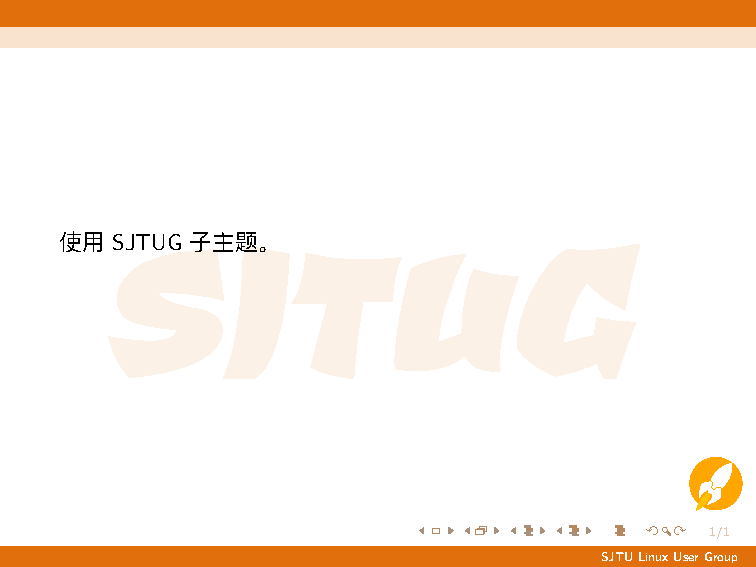
\includegraphics[width=|\only<1-3>{4cm}\only<4->{0.4\textbackslash{}textwidth}|]{sjtug}
|\highlightline<7>|  \caption{SJTUG 徽标}\label{fig:sjtug}
|\highlightline<5>|\end{figure}
\end{document}
      \end{codeblock}
    \end{column}
    \begin{column}{0.4\textwidth}
      \only<1>{
        \includepdflarge{support/examples/insertimage.pdf}
      }

      \only<2>{
        为了插入外部图片,需要使用 \pkg{graphicx} 宏包。之后在文档主体便可以使用 \cmd{includegraphics} 插入图片。导言区也可以加入 \cmd{graphicspath} 指定图片文件夹\footnotemark。
      }

      \only<3>{
        \cmd{includegraphics} 命令便以相对路径的方式插入图片,如果无同名图片,那么后缀名可以省略。可以使用可选参数指定插入的图片尺寸,最佳实践是使用 \cmd{textwidth} 或 \cmd{linewidth} 的相对值指定尺寸大小,以在未来可能的布局更改中保留一定的灵活性。
        \note{比如我未来想变更为幻灯片的时候。}
      }

      \only<4>{
        也可以通过键值对的方法设置图片的其他属性。
        \note{事实上,\LaTeX{} 很多命令都是使用方括号添加可选参数的。}
        \begin{center}
          \footnotesize
          \begin{tabular}{rl}
            \opt{width} & 宽度 \\
            \opt{height} & 高度 \\
            \opt{scale} & 缩放 \\
            \opt{angle} & 角度 \\
          \end{tabular}
        \end{center}
      }

      \only<5>{
        \env{figure} 为一个浮动体环境(\env{table} 也是),可以将其移动到其他位置上以减少行文中的空白。可以添加可选参数以指定如何放置浮动体,最多可以使用四种位置描述符:
        \begin{center}
          \footnotesize
          \begin{tabular}{cll}
            \opt{h} & Here & 尽可能在这里 \\
            \opt{t} & Top & 页面顶部 \\
            \opt{b} & Bottom & 页面底部 \\
            \opt{p} & Page & 浮动体专页 \\
          \end{tabular}
        \end{center}
        还可以只使用 \pkg{float} 宏包提供的 \opt{H} 描述符以强制置于此处。
      }

      \only<6>{
        采用 \cmd{centering} 命令而不是 \env{center} 环境来水平居中图片。这将避免多余的纵向间距。
      }

      \only<7>{
        使用 \cmd{caption} 命令输入题注,如果这个命令写在插入图片前面,题注将会在上方(中文中一般对 \env{table} 环境这么做)。后面将会看到如何对留有标记(\cmd{label})的图片进行引用。
      }
    \end{column}
  \end{columns}
  \only<2>{\footnotetext{其命令参数每个为一个以 \texttt{/} 结尾的文件夹,每个文件夹需要使用大括号包裹起来。}}
\end{frame}

\begin{frame}[fragile]
  \begin{columns}
    \begin{column}{0.6\textwidth}
      \begin{codeblock}[]{插入双图}
\documentclass{ctexart}
\usepackage{graphicx}
\graphicspath{{figs/}{pics/}}
\begin{document}
  \begin{figure}[ht]
|\highlightline<1>|    \begin{minipage}{0.48\textwidth}
      \centering
      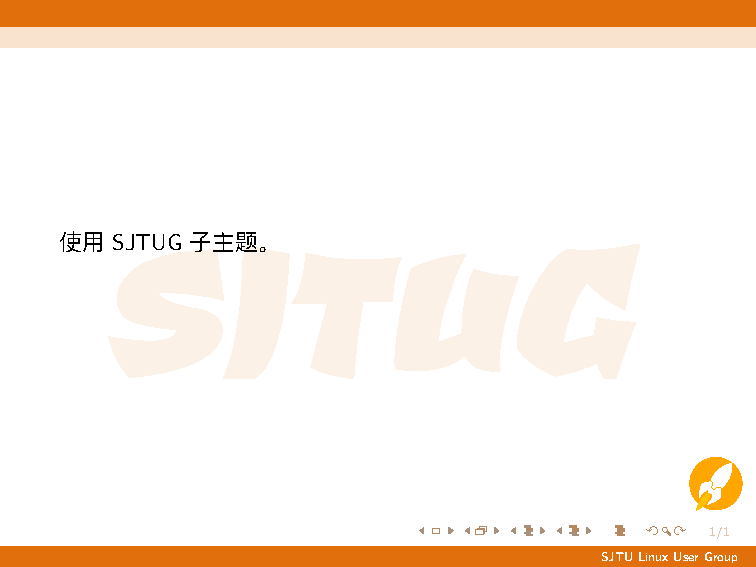
\includegraphics[height=2cm]{sjtug}
|\highlightline<2>|      \caption{SJTUG 徽标}\label{fig:sjtug}
|\highlightline<1>|    \end{minipage}\hfill
|\highlightline<1>|    \begin{minipage}{0.48\textwidth}
      \centering
      
\includegraphics[height=2cm]{sjtugt}
|\highlightline<2>|      \caption{SJTUG|\phantom{}|文字}\label{fig:sjtugt}
|\highlightline<1>|    \end{minipage}
  \end{figure}
\end{document}
      \end{codeblock}
    \end{column}
    \begin{column}{0.4\textwidth}

      \only<1>{
        在 \env{figure} 环境里使用 \env{minipage} 小页制作列盒子,以并排两图并分别编号,需要设定强制参数以指定列宽。两个小页之间添加 \cmd{hfill} 使两个小页两端对齐。
      }

      \only<2>{
        在每个小页内部分别使用 \cmd{caption} 添加标签。
      }

      \only<3>{
        \includepdflarge{support/examples/doubleimages.pdf}
      }
    \end{column}
  \end{columns}
\end{frame}

\begin{frame}[fragile]%
  \begin{columns}
    \begin{column}{0.6\textwidth}
      \begin{codeblock}[]{}
\documentclass{ctexart}
\usepackage{graphicx}
|\highlightline|\usepackage{subcaption}
\graphicspath{{figs/}{pics/}}
\begin{document}
  \begin{figure}[ht]
|\highlightline|    \begin{subfigure}{0.48\textwidth}
      \centering
      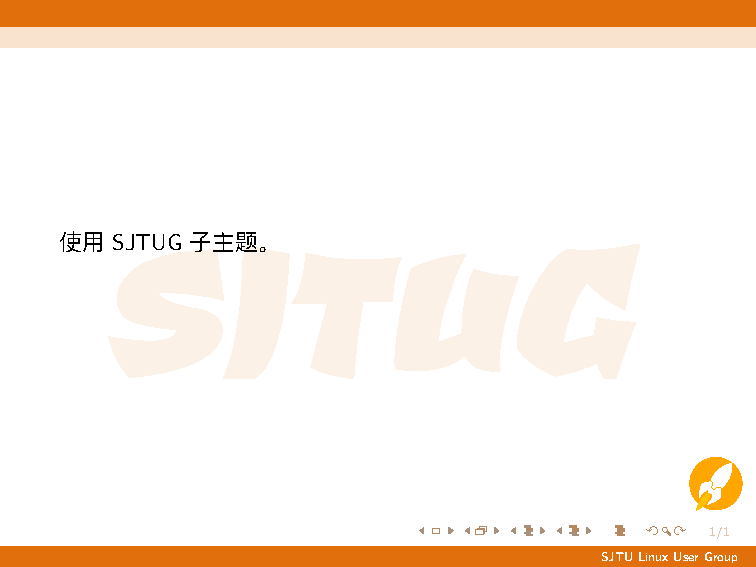
\includegraphics[height=2cm]{sjtug}
      \caption{|\phantom{}|徽标}
|\highlightline|    \end{subfigure}\hfill
|\highlightline|    \begin{subfigure}{0.48\textwidth}
      \centering
      
\includegraphics[height=2cm]{sjtugt}
      \caption{|\phantom{}|文字}
|\highlightline|    \end{subfigure}
    \caption{SJTUG}\label{fig:sjtug}
  \end{figure}
\end{document}
      \end{codeblock}
    \end{column}
    \begin{column}{0.4\textwidth}
      \includepdflarge{support/examples/subfigures.pdf}\vspace{15pt}
      \pkg{subcaption} 宏包提供了 \env{subfigure} 环境(以及 \env{subtable}),可以用于以子图的形式插入,编号会增加一级。也可以为子图添加子级引用编号。
    \end{column}
  \end{columns}
\end{frame}

\section{表}
\begin{frame}[fragile]
  \frametitle{简单表格}
  \begin{columns}
    \begin{column}{0.6\textwidth}
      \begin{codeblock}[]{}
\documentclass{ctexart}
|\only<1-2>{\highlightline}|\usepackage{|\temporal<1>{array}{\highlight{array}}{array},\temporal<2>{booktabs}{\highlight{booktabs}}{booktabs}|}
\begin{document}
\begin{table}[ht]
  \centering
  \caption{|\phantom{}|北京冬奥会吉祥物}
|\highlightline<1>|  \begin{tabular}{lp{3cm}}
|\highlightline<2>|    \toprule
|\highlightline<3>|吉祥物 & 描述                          \\
|\highlightline<2>|    \midrule
|\highlightline<3>|冰墩墩 & 2022 年北京冬季奥运会吉祥物  \\
|\highlightline<3>|雪容融 & 2022 年北京冬季残奥会吉祥物  \\
|\highlightline<2>|    \bottomrule
|\highlightline<1>|  \end{tabular}
\end{table}
\end{document}
      \end{codeblock}
    \end{column}
    \begin{column}{0.4\textwidth}
      
      \only<1>{
        使用 \env{tabular} 环境绘制表格。需要添加参数(称为\textbf{表格导言})以确定每一列的对齐方式。引入 \pkg{array} 宏包来使用更多的\textbf{引导符}。
        \begin{center}
          \footnotesize
          \begin{tabular}{>{\ttfamily}ll}
            \alert{l} & 向左对齐 \\
            \alert{c} & 居中对齐 \\
            \alert{r} & 向右对齐 \\
            \alert{p\{3cm\}} & 固定列宽,两端对齐 \\
            \alert{m\{3cm\}} & \texttt{p} + 垂直居中对齐 \\
            \alert{>\{\textbackslash{}bfseries\}} & 后一列单元格前加命令 \\
            \alert{*\{3\}\{l\}} & 三个左对齐列 \\
          \end{tabular}
        \end{center}
      }

      \only<2>{
        \pkg{booktabs} 宏包提供了标准三线表格所需要的行分割线:\cmd{toprule},\cmd{midrule},\cmd{bottomrule}。也可以使用 \cmd{cmidrule\{1-2\}} 来部分地绘制行分割线。一般不推荐在专业表格中使用纵向分割线。
      }

      \only<3>{
        每行内容使用 \textbackslash\textbackslash{} 分隔开,每行中的单元格使用 \& 分隔开。
      }

      \only<4>{
        \includepdflarge{support/examples/table.pdf}
      }
    \end{column}
  \end{columns}
\end{frame}

\begin{frame}[fragile]%
  \begin{columns}
    \begin{column}{0.6\textwidth}
      \begin{codeblock}[]{表头居中}
\documentclass{ctexart}
\usepackage{array,booktabs}
\begin{document}
\begin{table}[ht]
  \centering
  \caption{|\phantom{}|北京冬奥会吉祥物}
  \begin{tabular}{lp{3cm}}
    \toprule
|\highlightline|\multicolumn{1}{c}{|\phantom{}|吉祥物} &
|\highlightline|\multicolumn{1}{c}{|\phantom{}|描述} \\
    \midrule
|\phantom{}|冰墩墩 & 2022 年北京冬季奥运会吉祥物  \\
|\phantom{}|雪容融 & 2022 年北京冬季残奥会吉祥物  \\
    \bottomrule
  \end{tabular}
\end{table}
\end{document}
      \end{codeblock}
    \end{column}
    \begin{column}{0.4\textwidth}
      \cmd{multicolumn} 命令不仅可以用于合并同行的单元格,还可以用于临时地屏蔽表格导言对该列的对齐方式定义。这里用于居中表头。
      \begin{center}
        \parbox{0.85\linewidth}{
          \cmd{multicolumn\{格数\}\{对齐方式\}\{内容\}}
        }
      \end{center}
      跨页表格考虑使用 \pkg{longtable} 宏包。带标注的表格可以考虑使用 \pkg{threeparttable} 宏包。考虑使用在线工具生成表格代码 \link{https://www.tablesgenerator.com/latex_tables}。
      \note{复杂的使用方法在 \SJTUThesis{} 示例文档中都有提及。}
    \end{column}
  \end{columns}
\end{frame}

\section{数学公式}
\begin{frame}
  \frametitle{数学模式}
  \begin{alertblock}{}
  输入数学公式是 \LaTeX{} 的绝对强项,很多常见的公式服务依赖于一些轻量级渲染引擎比如 MathJax, K\kern-.3ex\raise.4ex\hbox{\footnotesize A}\kern-.3ex\TeX{}。但是它们实际上使用的是 \LaTeX{} 语法变种,也就是说并没有使用 \LaTeX{} 后端。所以不要期望有完全一致的输出。
  \end{alertblock}
  
  为了更好的获得数学公式输入支持,请使用 \hologo{AmS}math 宏包。数学模式分为两种:
  \begin{description}
    \item[行内模式] 一般通过一对美元符号(\$$\cdots$\$)标记,可以使用编辑器内建的符号表输入数学符号,也可以使用在线工具手写识别 \link{https://detexify.kirelabs.org/classify.html}。
    \item[行间模式] 一般通过 \env{equation} 环境\footnote{这是有编号环境,其加星号的变种 \env{equation*} 用于生成无编号环境。}输入。如果需要使用多行公式,请使用 \env{align} 环境,并按照类似表格输入的方式,使用 \& 对齐符号,\textbackslash\textbackslash{} 换行。如果不想手动居中,可以考虑多行自动居中的 \env{gather} 和单个大型公式首尾两端对齐 \env{multline}。
  \end{description}
  \note{关于表格和数学公式,如果不太熟悉如何输入,或者符号表记不住,推荐从比较容易上手的编辑器起步,比如 \TeX{}studio 提供了用户友好的界面(\faWindows{} 上的向导 $\rightarrow$ 数学助手)。我相信输入半年后,就可以对这些符号的输入很熟练了。
  
  你会发现我的这套教程没有讲很多的数学公式输入技巧,因为这些东西只有你自己熟练了才能体会。而且 \LaTeX{} 本来就不是完全关于数学公式的。}
\end{frame}

\begin{frame}
  \frametitle{数学命令展示}
  \begin{columns}
    \begin{column}{0.33\textwidth}
      \begin{exampleblock}{}
        $PV=nRT$
      \end{exampleblock}
      \begin{exampleblock}{}
        $\sum_{i=1}^ki^2=\frac{n(n+1)(2n+1)}{6}$
      \end{exampleblock}
      \begin{exampleblock}{}
        $T(n) = aT\left(\left\lceil\frac{n}{b}\right\rceil\right) + \mathcal{O}(n^d)$
      \end{exampleblock}
      \begin{exampleblock}{}
        $\frac{x_{1}+x_{2}+x_{3}}{3}\geq \sqrt[3]{x_{1}x_{2}x_{3}}$
      \end{exampleblock}
      \begin{exampleblock}{}
        $n=(\underbrace{1\cdots 1}_{k\text{ of 1's}})_2=2^{k+1}-1$
      \end{exampleblock}
      \begin{exampleblock}{}
        $\nabla f (P)= \left.\left(\frac{\partial f}{\partial x},\frac{\partial f}{\partial y},\frac{\partial f}{\partial z}\right)\right|_{P}$
      \end{exampleblock}
    \end{column}
    \begin{column}{0.67\textwidth}
      \begin{exampleblock}{}
        \begin{equation*}
          \int_{a}^b f(x)\,\mathrm{d}x=\lim_{|P|\rightarrow 0}\sum_{i=1}^n f(\xi_i)\Delta x_i
        \end{equation*}
      \end{exampleblock}
      \begin{exampleblock}{}
        \begin{equation}
          T(n) = \begin{cases}
            \mathcal{O}(n^d),&\textrm{if } d>\log_b a, \\
            \mathcal{O}(n^d\log n), &\textrm{if } d=\log_b a,\\
            \mathcal{O}(n^{\log_b a}), &\textrm{if } d<\log_b a.
          \end{cases}
        \end{equation}
      \end{exampleblock}
      \begin{exampleblock}{}
        \begin{align}
          Q^{T}A&=R \\
          \begin{pmatrix}
            q_1^T \\ q_2^T \\ q_3^T
          \end{pmatrix}
          \begin{pmatrix}
            a_1 & a_2 & a_3
          \end{pmatrix}
          &=R
        \end{align}
      \end{exampleblock}
    \end{column}
  \end{columns}
  \note{关于如果 \LaTeX{} 报出了错误,比如说数学模式下不能有空行,想要学习如何修复这些错误,
  可以详见 Learn\LaTeX{}.org 的相关章节
  \link{https://github.com/CTeX-org/learnlatex.github.io/blob/zh-Hans/zh-Hans/lesson-15.md}。}
\end{frame}

%更深入地讲解 mathtools, unicode-math, siunix

\section{引用}
\begin{frame}[fragile]
  \frametitle{交叉引用}
  \only<1>{
    正如之前所提到的,\LaTeX{} 中使用 \cmd{label} 标记,然后可以使用 \cmd{ref} 来引用这个标记。 \cmd{label} 可以放在使用计数器的对象之后。
  }

  \only<2>{
    为了使得对公式编号的引用带有括号,推荐使用 \hologo{AmS}math 宏包中的 \cmd{eqref} 命令。对于多行公式环境,每一个换行符前都可以添加一个 \cmd{label} 用于引用该行公式。
  }
  
  \begin{columns}
    \begin{column}{0.5\textwidth}
      \begin{codeblock}[]{图}
\begin{figure}
|\highlightline<1>|  \caption{|\phantom{}|示例}\label{fig:example}
\end{figure}
      \end{codeblock}
      \begin{codeblock}[]{表}
\begin{table}
|\highlightline<1>|  \caption{|\phantom{}|示例}\label{tab:example}
\end{table}
      \end{codeblock}
    \end{column}
    \begin{column}{0.5\textwidth}
\begin{codeblock}[]{目次}
|\highlightline<1>|\section{|\phantom{}|示例}\label{sec:example}
\end{codeblock}

\begin{codeblock}[]{公式}
\begin{equation}
  a = b + c
|\highlightline<1>|\label{eq:example}
\end{equation}
|\highlightline<2>|如公式 \eqref{eq:example} 所示,
\end{codeblock}
    \end{column}
  \end{columns}
\end{frame}

\begin{frame}[fragile]
  \frametitle{文献引用}
  \LaTeX{} 可以通过专用数据库文件 \texttt{.bib} 自动生成参考文献,很多的文献管理文件比如 EndNote \link{https://lic.sjtu.edu.cn/Default/softshow/tag/MDAwMDAwMDAwMLGImKE}, Zotero \link{https://www.zotero.org/}, JabRef \link{https://www.jabref.org/} 都可以直接导出这种格式的文件用于 \LaTeX{} 论文中的引用。一般不需要手写数据库文件,你只需要注意每一个文献会在数据库中有一个主键,这个类似于上文的 \cmd{label} 标记,只是要引用数据库中的文献需要使用 \cmd{cite} 命令。
  
  \begin{codeblock}[]{ref.bib}
|\highlightline|@article{devoftech,|\hfill\alert{\% 类型为期刊论文,主键为\texttt{devoftech}}|
  title={|\phantom{}|新时期我国信息技术产业的发展},
  author={|\phantom{}|江泽民},
  year={2008}
}
  \end{codeblock}
\end{frame}

\begin{frame}
  \frametitle{文献引用}
  而让 \LaTeX{} 处理 \texttt{.bib} 数据库文件与引用有两种工作流。你可能需要查清楚如何在编辑器中设置对应的工作流,或者采用后面所提到的高级编译方式 \texttt{latexmk}。
  \begin{columns}
    \begin{column}{0.5\textwidth}
      \begin{block}{\hologo{BibTeX} + \pkg{natbib}}
        一般期刊提交使用这种方法,\pkg{natbib} 宏包将提供命令 \cmd{citet}(文本引用) 和 \cmd{citep}(括号引用)。
      \end{block}
      \begin{alertblock}{\hologo{BibTeX} + \pkg{gbt7714}}
        中文引用可以直接使用 \pkg{gbt7714} 宏包,但是角模式和正文模式不能混用。
      \end{alertblock}
    \end{column}
    \begin{column}{0.5\textwidth}
      \begin{block}{\hologo{biber} + \pkg{biblatex}}
        这是更容易自定义的方法,与 \hologo{BibTeX} 的运作方式稍有不同。\pkg{biblatex} 提供了更加智能的引用命令。
      \end{block}
      \begin{alertblock}{\hologo{biber} + \pkg{biblatex-gb7714-2015}}
        而中文引用可以使用 \pkg{biblatex} 宏包的样式 \pkg{gb7714-2015}。
      \end{alertblock}
    \end{column}
  \end{columns}
\end{frame}

\begin{frame}[fragile]
  \frametitle{文献引用}
  \begin{columns}
    \begin{column}{0.5\textwidth}
      \begin{codeblock}[]{\hologo{BibTeX} + \pkg{gbt7714}}
\documentclass{ctexart}
\usepackage{gbt7714}
\bibliographystyle{gbt7714-numerial}
% \citestyle{numbers}  % 正文模式
\begin{document}
  |\phantom{}|他指出了...\cite{devoftech}
  \bibliography{ref}
\end{document}
      \end{codeblock}
    \end{column}
    \begin{column}{0.5\textwidth}
      \begin{codeblock}[]{\hologo{biber} + \pkg{biblatex-gb7714-2015}}
\documentclass{ctexart}
\usepackage[backend=biber,style=gb7714-2015]{biblatex}
\addbibresource{ref.bib}
\begin{document}
  |\phantom{}|他在文献 \parencite{devoftech}
  |\phantom{}|指出了...\cite{devoftech}
  \printbibliography
\end{document}
      \end{codeblock}
    \end{column}
  \end{columns}
\end{frame}

\begin{frame}
  \frametitle{文献引用}
  \begin{columns}
    \begin{column}{0.5\textwidth}
      \includepdflarge{support/examples/bibtex.pdf}
    \end{column}
    \begin{column}{0.5\textwidth}
      \includepdflarge{support/examples/biblatex.pdf}
    \end{column}
  \end{columns}
  \note{这页有一篇上过《新闻联播》的论文。}
\end{frame}

\end{shadedsection}

  % !TeX root = ../../latex-talk.tex

\part{SJTUThesis}

\begin{frame}
  \frametitle{本部分主要参考}
  \begin{bibliolist}{00}
    \onlineitem \textsc{SJTUG}.
    \newblock \textsc{SJTUThesis} 示例文档[EB/OL].
    \newblock 2022. \url{https://github.com/sjtug/SJTUThesis}.

    \onlineitem \textsc{SJTUG}.
    \newblock \textsc{SJTUThesis} 用户文档[EB/OL].
    \newblock 2022. \url{https://github.com/sjtug/SJTUTeX}.
  \end{bibliolist}
\end{frame}

\begin{frame}
  \frametitle{简介}
  \begin{columns}
    \begin{column}{0.6\textwidth}
      \begin{itemize}
        \item 最早由韦建文于 2009 年 11 月发布 0.1a 版
        \item 2018 年起由 SJTUG 接手维护
        \item 2019 年 6 月吴伟健重构了整个宏包的代码,升级版本号为 1.0
        \item 2022 年 11 月模板改版后,吴伟健、张驰等人使用 \LaTeX3 重构 2.0 版本
        \item 最新版:\SJTUThesisVersion{} (\SJTUThesisDate)
        \item 支持本科、硕士、博士学位论文的排版
        \item 推荐使用最新版本的 \TeX{} 发行版编译
      \end{itemize}
    \end{column}
    \begin{column}{0.4\textwidth}
      \begin{exampleblock}{}
        \begin{minipage}[c]{1cm}
          \includegraphics[width=0.8cm]{\getcontribpath{sjtug}{vi/sjtug}}
        \end{minipage}
        \begin{minipage}[c]{3cm}
          \href{https://github.com/sjtug}{sjtug}/\href{https://github.com/sjtug/SJTUThesis}{SJTUThesis}
        \end{minipage}
      \end{exampleblock}
      \vspace{-8pt}
      \begin{block}{}
        \scriptsize
        上海交通大学 \hologo{XeLaTeX} 学位论文及课程论文模板 | Shanghai Jiao Tong University \hologo{XeLaTeX} Thesis Template
      \end{block}
      \vspace{-8pt}
      \begin{alertblock}{}
        \scriptsize
        \begin{tabular}{cl}
          \faStar & 2.6k \\
          \faEye & 52 \\
          \faCodeBranch & 726 \\
        \end{tabular}
      \end{alertblock}
    \end{column}
  \end{columns}
\end{frame}

\begin{frame}
  \frametitle{\only<1>{为什么使用 \LaTeX{} 排版论文?}\only<2>{当然它们也互相学习}}
  \begin{columns}[t]
    \begin{column}{0.25\textwidth}
      \begin{exampleblock}{\faMarkdown{} Markdown}
        \begin{itemize}
          \item[\faPlus] 技术文档流行
          \item[\faPlus] 语法简单 
          \item[\faMinus] 不内置格式控制
        \end{itemize}
      \end{exampleblock}
      \only<2>{
        \begin{block}{}
          \begin{itemize}
            \item[\faBolt] R Markdown (Bookdown) 模板 \link{https://github.com/bubifengyun/SJTUThesis-Rmd} \link{https://github.com/bubifengyun/SJTUThesis-Rmd}
            \item[\faAsterisk] 配套 MathJax 渲染公式  
          \end{itemize}
        \end{block}
      }
    \end{column}
    \begin{column}{0.25\textwidth}
      \begin{exampleblock}{\faFileWord{} Word}
        \begin{itemize}
          \item[\faPlus] 通用论文格式
          \item[\faPlus] 所见即所得
          \item[\faMinus] 进阶排版仍困难 
        \end{itemize}
      \end{exampleblock}
      \only<2>{
        \begin{block}{}
          \begin{itemize}
            \item[\faBolt] 数学公式可以直接通过 \LaTeX{} 格式转换
            \item[\faAsterisk] 也就是 Unicode Math 输入方式 
          \end{itemize}
        \end{block}
      }
    \end{column}
    \begin{column}{0.25\textwidth}
      \begin{block}{\LaTeX{} SJTUThesis}
        \begin{itemize}
          \item[\faPlus] 学术论文格式
          \item[\faPlus] 内容样式分离
          \item[\faMinus] 上手有门槛 
        \end{itemize}
      \end{block}
      \only<2>{
        \begin{exampleblock}{}
          \begin{itemize}
            \item[\faBolt] \TeX{} 的可视前端 \hologo{LyX} \link{https://www.lyx.org/Download} Overleaf Rich Text 模式
            \item[\faAsterisk] \TeX{} 的可视改良 \TeX{}\raise-0.25em\hbox{\footnotesize MACS} \link{http://texmacs.org/tmweb/home/welcome.en.html} \link{https://mogan.app}
          \end{itemize}
        \end{exampleblock}
      }
    \end{column}
    \begin{column}{0.25\textwidth}
      \begin{exampleblock}{\faAdobe{} InDesign}
        \begin{itemize}
          \item[\faPlus] 专业杂志排版
          \item[\faPlus] 精细调整
          \item[\faMinus] 过于繁琐专业  
        \end{itemize}
      \end{exampleblock}
      \only<2>{
        \begin{block}{}
          \begin{itemize}
            \item[\faBolt] 传说用了 \TeX{} 的一些算法 \link{https://mp.weixin.qq.com/s/GASGHK-GsIg2Fwb2jWwpvw}
          \end{itemize}
        \end{block}
      }
    \end{column}
  \end{columns}
  \note{\emph{这页仅作简要介绍。}

  让我们来讨论 the elephant in the room:为什么用 \LaTeX{} 排版论文?
  }
  \note<1>[item]{Markdown 很好啊,方便的语法,一般技术文档也常用。但就是因为它太简单了,没有内置样式控制,一般需要借助 HTML,CSS 那一套东西。}
  \note<2>[item]{也会有一些人尝试通过 R Markdown(Bookdown)改进,当然你也可以试着使用 \LaTeX{} 里的 \pkg{markdown} 宏包
  (这有点像各种前端博客框架渲染 Markdown 为 HTML,只不过这里渲染 \LaTeX{} 生成 PDF,代码抄录方面已经有 Sphinx 这个工具 \link{https://github.com/sphinx-doc/sphinx}),
  以及可以通过 MathJax 渲染 \TeX{} 公式。
  }
  \note<1>[item]{Word 很好啊,官方钦定的论文写作方法,可见即可得,但是进阶排版仍然可以困难。就拿排版公式来说,
  大家以前初高中学的、或者是计算机二级考的 Word 2003 要排版公式,一种是装 MathType 插件,版本间不兼容、一种是搞个域代码+替换字体。}
  \note<2>[item]{Word 2007 之后添加了插入正经的 Unicode 公式功能,但默认的 Calibri Math 字体以及符号布局仍然赶不上 \TeX{} 的美感。
  }
  \note<1>[item]{根据之前学到的一些技巧,看起来不难对吧(虽然有我诱导的成分),然后它内容与样式分离的设计理念已经渗入了很多领域。以及很多学术论文都需要 \LaTeX{} 的提交。}
  \note<2>[item]{当然现在也推出了可见即可得的编辑器 \hologo{LyX},Overelaf 的可视模式(虽然这两个并不是一个东西);以及迟先生很喜欢的 TeXmacs,一种不使用 \TeX{} 底层的、但是效果相像的排版程序。
  }
  \note<1>[item]{设计相关专业的同学可能更喜欢 Adobe Indesign,对图文混排更为擅长。但是它也足够复杂,虽然提供了几乎所有的排版用具,但是我还没见过用它排版几十页充满公式的论文的(或许有人会开先河?)。}
  \note<2>[item]{以及传说它用了 \TeX{} 的一些算法,所以 \TeX{} 还是老大哥,兼具美感和批量化处理的折中方法。}
\end{frame}

\begin{frame}
  \frametitle{开始使用}
  \alert{下载} 推荐安装 Git \link{https://git-scm.com/} 后,克隆 SJTUG 镜像仓库
  \begin{exampleblock}{\faGit*}
    \ttfamily\small
    git clone https://mirror.sjtu.edu.cn/git/SJTUThesis.git/
  \end{exampleblock}

  \alert{编译} 推荐使用 \pkg{latexmk} 编译\footnote{\hologo{MiKTeX} 用户需要手动安装 Perl 解释器 \link{https://www.perl.org/get.html} 才能使用 \pkg{latexmk}。},在不能够利用自带的 \texttt{.latexmkrc} 配置文件的情况下,需要查清楚在对应的编辑器中如何使用 \hologo{XeLaTeX} + \hologo{biber} 编译\footnote{这种情况下,你可能需要查清楚如何全局安装该文档类,并刷新文件名数据库。} \link{https://github.com/sjtug/SJTUThesis/blob/master/README.md}。
  \begin{exampleblock}{\faTerminal}
    \ttfamily\small
    latexmk -xelatex main
  \end{exampleblock}

  \alert{在线} 直接使用 Overleaf 链接 \link{https://www.overleaf.com/latex/templates/sjtuthesis-latex-thesis-template-for-shanghai-jiao-tong-university/mkdwbyjbtfgg?r=sdkbtJ4qGS8kDZQQ&rm=d&rs=b}。
  其他在线平台用户可以下载压缩包,上传至对应平台并采用 \hologo{XeLaTeX} 编译,请注意使用最新版本的 \TeX{} Live。
  \note{不会 Git 的同学可以直接 Download ZIP。}
\end{frame}

\begin{frame}
  \frametitle{手动编译}
  \alert{第一次编译失败} 如果没有办法通过通常方式编译成功,请尝试使用文件夹内附带 \faLinux{}\,\faApple{} \texttt{Makefile} 和 \faWindows{} \texttt{Compile.bat} 进行编译。

  \alert{统计字数} 编写过程中也可以使用对应的命令调用 \TeX{}count 来统计正文字数。
  \begin{columns}
    \begin{column}{0.38\textwidth}
      \begin{exampleblock}{\faLinux{}\,\faApple}
        \ttfamily
        make all\\
        make clean\\
        make cleanall\\
        make wordcount
      \end{exampleblock}
    \end{column}
    \begin{column}{0.38\textwidth}
      \begin{exampleblock}{\faWindows}
        \ttfamily
        ./Compile.bat thesis\\
        ./Compile.bat clean\\
        ./Compile.bat cleanall\\
        ./Compile.bat wordcount
      \end{exampleblock}
    \end{column}
    \begin{column}{0.24\textwidth}
      \begin{block}{\faInfo}
        \ttfamily
        编译论文\\
        清理中间文件\\
        $\hookrightarrow +$删除论文\\
        统计字数
      \end{block}
    \end{column}
  \end{columns}
\end{frame}

\begin{frame}[label=compile]
  \frametitle{编译问题排查}
  \begin{columns}
    \begin{column}{0.33\textwidth}
      \begin{alertblock}{无法使用 \texttt{latexmk}\thesisissue{578}}
        \hologo{MiKTeX} 需要安装 Perl 解释器。
      \end{alertblock}  
      \begin{alertblock}{\CTeX{} 套装无法编译\thesisissue{446}}
        使用最新 \TeX{} 发行版。\link{https://github.com/Aloft-Lab/CTeX-Installer}
      \end{alertblock}
      \begin{alertblock}{\hologo{pdfLaTeX} 无法编译\thesisissue{444}}
        请使用 \texttt{latexmk},或更改编辑器设置以 \hologo{XeLaTeX} 编译。
      \end{alertblock}
    \end{column}
    \begin{column}{0.33\textwidth}
      \begin{alertblock}{缺少字体\thesisissue{564} \thesisdiscuss{598}}
        更换字体集,或者安装对应字体。
      \end{alertblock}
      \begin{alertblock}{缺少汉字\thesisissue{533} \thesisdiscuss{617}}
        去除使用 fandol 字体集的设定。或者是安装字体后,改用 \texttt{cjk-font=adobe} 或 \texttt{cjk-font=founder}。
      \end{alertblock}
    \end{column}
    \begin{column}{0.33\textwidth}
      \begin{block}{\faInfoCircle{} README}
        不同编辑器的设置请首先参阅 README \link{https://github.com/sjtug/SJTUThesis/blob/master/README.md} 文档。
      \end{block}
      \begin{block}{\faBookOpen{} Wiki}
        其他编译问题推荐查阅 Wiki \link{https://github.com/sjtug/SJTUThesis/wiki} 的使用说明部分。
      \end{block}
    \end{column}
  \end{columns}
  \note{两个进阶问题:
  
  如果之前出现了编译错误,在重新编译前,最好清理一下临时文件(\texttt{make clean})。

  如果是 biber 出现了问题,还可以尝试 \texttt{rm -rfv \$(biber --cache)}。\thesisdiscuss{774}
  }
\end{frame}

\begin{frame}[label=covers]
  \frametitle{论文组成}
  \begin{figure}[h]
    \centering
    \foreach \thesispage/\thesisnote in {
      1/{中文封面},3/{英文封面},5/{版权页},7/{中文摘要},9/{英文摘要},11/{目录},13/{插图目录},15/{表格目录},
      17/{正文},27/{参考文献},29/{附录},31/{成果},33/{致谢},35/{大摘要}} {%
      \begin{subfigure}{.13\textwidth}
        \centering
        \fzerobox{\includegraphics[width=\textwidth,page=\thesispage]{support/thesis/sample-thesis-zh.pdf}}
        \caption{\thesisnote}
      \end{subfigure}
    }
  \end{figure}
  \note{虽然说符号表在新版中是要放在附录中,但是学位论文规范中却说可以放在正文前,所以你可以自行选择。}
  \note{文档中的彩色框是标识超链接,印刷时不会输出,如果希望关闭可以向 \pkg{hyperref} 宏包添加可选参数 \opt{hidelinks}。}
\end{frame}

\begin{frame}[fragile]
  \frametitle{文档类选项}
  \begin{columns}
    \begin{column}{0.35\textwidth}
      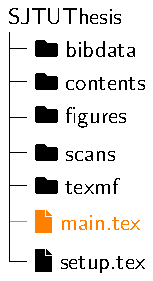
\includegraphics[page=1]{support/figures/thesisdir.pdf}
    \end{column}
    \begin{column}{0.65\textwidth}
      文档类选项是指在载入文档类时的可选选项,多个选项使用逗号隔开,文档类选项会对所有宏包可见。
      \begin{codeblock}[escapechar="]{main.tex}
% !TeX encoding = UTF-8

% 载入 SJTUThesis 模版
"\highlightline"\documentclass[type=master]{sjtuthesis}
% 选项
%   type=[doctor|master|bachelor],
%   zihao=[-4|5],
%   lang=[zh|en],
%   review,
%   [twoside|oneside],
%   math-style=[ISO|TeX],
      \end{codeblock}
    \end{column}
  \end{columns}
\end{frame}

\begin{frame}[fragile]
  \frametitle{文档类选项}
  \begin{columns}
    \begin{column}{0.3\textwidth}
      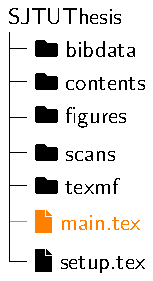
\includegraphics[page=1]{support/figures/thesisdir.pdf}
    \end{column}
    \begin{column}{0.7\textwidth}
      我是学士,写英文论文
      \begin{codeblock}[]{}
|\phantom{}|\documentclass[type=bachelor,lang=en]{sjtuthesis}
      \end{codeblock}
      我是硕士,盲审
      \begin{codeblock}[]{}
|\phantom{}|\documentclass[type=master,review]{sjtuthesis}
      \end{codeblock}
      我是博士,先写着电子版不空页
      \begin{codeblock}[]{}
|\phantom{}|\documentclass[type=doctor,oneside]{sjtuthesis}
      \end{codeblock}
    \end{column}
  \end{columns}
  \note{有 ChatGPT 那味了。}
\end{frame}

\begin{frame}
  \frametitle{文档类选项}
  \begin{columns}
    \begin{column}{0.35\textwidth}
      \includegraphics[page=2,scale=0.9]{support/figures/thesisdir.pdf}
    \end{column}
    \begin{column}{0.65\textwidth}
      \begin{table}
        \caption{文档类选项}
        \footnotesize
        \begin{tabular}{>{\ttfamily}rll}
          \toprule
          选项 & 含义 & 相关 \\
          \midrule
          type= & 指定论文类型 & 第 \ref{covers} 页\\
          \midrule
          cjk-font= & 指定中文字体 & \\
          text-font= & 指定西文字体 & 第 \ref{frame:fonts} 页\\
          math-font= & 指定数学字体 & \\
          math-style= & 指定数学样式 & 第 \ref{frame:math-style} 页\\
          \midrule
          review & 开启盲审模式 & \thesisissue{195} \thesisissue{686} \\
          twoside & 双页模式 & \thesisissue{554} \\
          oneside & 单页模式 & \thesisissue{694} \\
          openright & 章从奇数页开始 & \thesisdiscuss{724} \\
          openany & 章从任意页开始 & \thesisissue{446} \\
          \bottomrule
        \end{tabular}
      \end{table}

      更多文档类选项查阅 \textsc{SJTU\TeX{}} 的开发文档 \link{https://github.com/sjtug/SJTUTeX/releases/download/v1.1.0/sjtuthesis.pdf}。
    \end{column}
  \end{columns}
\end{frame}

\begin{frame}[label={frame:fonts}]
  \frametitle{字体配置}
  \newcommand{\noticemark}{\alert{\normalshape \textopenbullet}}
  \begin{columns}
    \begin{column}{0.35\textwidth}
      \includegraphics[page=3,scale=0.9]{support/figures/thesisdir.pdf}
    \end{column}
    \begin{column}{.65\textwidth}
      相较于 \CTeX{} 使用 \texttt{fontset} 设定中文字体集,
      \SJTUThesis{} 还提供了西文、数学字体集的设定\footnotemark。

      {
        \medskip
        \ttfamily\scriptsize
        \alert{cjk-font=...\hfill 中文字体}
        
        \stamphrule\medskip

        \foreach \sjtufontname/\sjtufontdesc in {adobe/{adobe \faAdobe\noticemark},{fandol}/{fandol \faLinux{} \noticemark},{founder},mac/{mac \faApple{} \noticemark},windows/{windows \faWindows},ubuntu/{ubuntu \noticemark}}{
          \begin{minipage}{2.2cm}
            \centering
            \includefontpreview{support/thesis/cjkfont-\sjtufontname.pdf}\\
            \raisebox{0.8ex}{\sjtufontdesc}
          \end{minipage}
        }

        \bigskip

        \alert{text-font=..., math-font=...\hfill 西文与数学字体}

        \stamphrule\medskip

        \foreach \sjtufontname/\sjtufontdesc in {{cambria}/{cambria \noticemark},{lm},{newcm}/{newcm \noticemark},{newpx},{newtx},{stixtwo}/{stixtwo \noticemark},{times},{xits}/{xits \noticemark}}{
          \begin{minipage}{2cm}
            \centering
            \includefontpreview{support/thesis/latinfont-\sjtufontname.pdf}\\
            \raisebox{0.8ex}{\sjtufontdesc}
          \end{minipage}
        }
      }
    \end{column}
  \end{columns}
  \footnotetext{\noticemark 表示无法使用 pdf\LaTeX{} 编译。}
\end{frame}

\begin{frame}[label={frame:math-style}]
  \frametitle{数学样式}
  \begin{columns}
    \begin{column}{0.35\textwidth}
      \includegraphics[page=2,scale=0.9]{support/figures/thesisdir.pdf}
    \end{column}
    \begin{column}{0.65\textwidth}
      新增数学样式 \texttt{math-style} 文档类选项,现在默认为 \texttt{ISO},
      如果更喜欢原始的 \TeX{} 数学样式,可以切换为 \texttt{TeX}。

      \begin{minipage}[c]{10em}
        \texttt{math-style=ISO}
      \end{minipage}
      \begin{minipage}[c]{5cm}
        \includemathstylepreview{support/thesis/mathstyle-ISO.pdf}
      \end{minipage}
       
      \begin{minipage}[c]{10em}
        \texttt{math-style=TeX}
      \end{minipage}
      \begin{minipage}[c]{5cm}
        \includemathstylepreview{support/thesis/mathstyle-TeX.pdf}
      \end{minipage}

      \begin{block}{}
        请注意在默认情况下(\texttt{math-style=ISO})应当使用 \cmd{increment} 而不是 \cmd{Delta} 表示有限增量。
      \end{block}
    \end{column}
  \end{columns}
\end{frame}

\begin{frame}[fragile]
  \frametitle{基本配置}
  \begin{columns}
    \begin{column}{0.35\textwidth}
      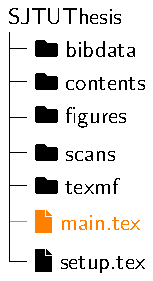
\includegraphics[page=1]{support/figures/thesisdir.pdf}
    \end{column}
    \begin{column}{0.65\textwidth}

      \only<1>{
        在 \texttt{main.tex} 中引入 \texttt{setup.tex} 来导入主要的信息录入与宏包加载配置。
      }

      \only<2>{
        \alert{\textbf{(a,b)}} 其中 \cmd{sjtusetup}(第 \ref{sjtusetup} 页)中的 \opt{info} 将会修改封面的信息设置。
      }

      \begin{codeblock}[firstnumber=12]{main.tex}
|\highlightline<1>|% 论文基本配置,加载宏包等全局配置
|\highlightline<1>|\input{setup}

\begin{document}

%TC:ignore

|\highlightline<2>|% 标题页
|\highlightline<2>|\maketitle
      \end{codeblock}
    \end{column}
  \end{columns}
\end{frame}

\begin{frame}[fragile, label=sjtusetup]
  \frametitle{基本配置}
  \begin{columns}
    \begin{column}{0.35\textwidth}
      \includegraphics[page=4]{support/figures/thesisdir.pdf}
    \end{column}
    \begin{column}{0.65\textwidth}
      \vspace*{-0.2cm}
      \begin{codeblock}[firstnumber=3]{setup.tex}
\sjtusetup{
  info = {
    zh/title  = {|\phantom{}|上海交通大学学位论文 \LaTeX{} 模板示例文档},
    en/title  = {A Sample for \LaTeX-based SJTU Thesis Template},
    zh/author = {|\phantom{}|某\quad{}某},
    en/author = {Mo Mo},
  },
  style = { float-seperator = {--}, },
  name = {
    achv = {|\phantom{}|攻读学位期间完成的论文},
  },
}
      \end{codeblock}
    \end{column}
  \end{columns}
\end{frame}

\begin{frame}[label=setup]
  \frametitle{基本配置}
  \begin{columns}
    \begin{column}{0.35\textwidth}
      \includegraphics[page=4]{support/figures/thesisdir.pdf}
    \end{column}
    \begin{column}{0.65\textwidth}
      \begin{table}
        \centering
        \caption{info 域}
        \footnotesize
        \begin{tabular}{lll} \toprule
          命令作用     & 中文对应选项                      & 英文对应选项                 \\ \midrule
          论文标题     & \texttt{zh/title}                 & \texttt{en/title}            \\
          关键字列表   & \texttt{zh/keywords}              & \texttt{en/keywords*}        \\
          作者姓名     & \texttt{zh/author}                & \texttt{en/author}           \\
          申请学位名称 & \texttt{zh/degree}                & \texttt{en/degree}           \\
          院系名称     & \texttt{zh/department}            & \texttt{en/department}       \\
          专业名称     & \texttt{zh/major}                 & \texttt{en/major}            \\
          导师         & \texttt{zh/supervisor}            & \texttt{en/supervisor}       \\
          副导师       & \texttt{zh/assoc-supervisor}      & \texttt{en/assoc-supervisor} \\
          联培导师     & \texttt{zh/co-supervisor}         & \texttt{en/co-supervisor}    \\
          日期         & \multicolumn{2}{c}{\texttt{date}}                                \\
          学号         & \multicolumn{2}{c}{\texttt{id}}                                  \\ \bottomrule
        \end{tabular}
      \end{table}
    \end{column}
  \end{columns}
  \note{有些选项是 v2 更名或新增的。}
  \note{注意现在使用语言前缀作为键名。}
\end{frame}

\begin{frame}[fragile]
  \frametitle{版权页}
  \begin{columns}
    \begin{column}{0.4\textwidth}
      \includegraphics[page=5]{support/figures/thesisdir.pdf}
    \end{column}
    \begin{column}{0.6\textwidth}
      \alert{\textbf{(c)}} \cmd{copyrightpage} 可以用于插入版权页。
      也可接受一个可选参数,用于直接使用扫描件,此时需要载入 \pkg{pdfpages} 包。\thesisissue{473}

      \begin{codeblock}[firstnumber=22]{main.tex}
% 原创性声明及使用授权书
\copyrightpage
% 插入外置原创性声明及使用授权书
% 导言区添加 \usepackage{pdfpages}
% \copyrightpage[scans/sample-copyright-old.pdf]
      \end{codeblock}
    \end{column}
  \end{columns}
\end{frame}

\begin{frame}[fragile]
  \frametitle{三个部分}
  \framesubtitle{前置部分}
  \begin{columns}
    \begin{column}{0.4\textwidth}
      \includegraphics[page=8]{support/figures/thesisdir.pdf}
    \end{column}
    \begin{column}{0.6\textwidth}
      \alert{\textbf{(d,e,f,g,h)}} 前言从 \cmd{frontmatter} 处开始,页码设置为大写罗马数字,主要包含摘要和目录内容。
      \begin{codeblock}[firstnumber=27]{main.tex}
|\highlightline|% 前置部分
|\highlightline|\frontmatter

% 摘要
\input{contents/abstract}

% 目录
\tableofcontents
% ...
      \end{codeblock}
    \end{column}
  \end{columns}
\end{frame}

\begin{frame}[fragile]
  \frametitle{三个部分}
  \framesubtitle{正文部分}
  \begin{columns}
    \begin{column}{0.4\textwidth}
      \includegraphics[page=9]{support/figures/thesisdir.pdf}
    \end{column}
    \begin{column}{0.6\textwidth}
      \alert{\textbf{(i,j,k)}} 正文从 \cmd{mainmatter} 处开始,页码设置为正常数字,包含正文、参考文献、附录内容。
      \begin{codeblock}[firstnumber=47]{main.tex}
|\highlightline|% 主体部分
|\highlightline|\mainmatter

% 正文内容
\input{contents/intro}
\input{contents/math_and_citations}
\input{contents/floats}
\input{contents/summary}

%TC:ignore

% 参考文献
\printbibliography[heading=bibintoc]

% 附录
\appendix
      \end{codeblock}
    \end{column}
  \end{columns}
\end{frame}

\begin{frame}[fragile]
  \frametitle{三个部分}
  \framesubtitle{结尾部分}
  \begin{columns}
    \begin{column}{0.4\textwidth}
      \includegraphics[page=10]{support/figures/thesisdir.pdf}
    \end{column}
    \begin{column}{0.6\textwidth}
      \alert{\textbf{(k,l,m,n)}} 结尾从 \cmd{backmatter} 处开始,页码设置为正常数字,包含致谢等相关情况。
      \begin{codeblock}[firstnumber=71]{main.tex}
|\highlightline|% 结尾部分
|\highlightline|\backmatter

% 用于盲审的论文需隐去致谢、发表论文、科研成果、简历

% 致谢
\input{contents/acknowledgements}

% 发表论文及科研成果
% 盲审论文中,发表论文及科研成果等仅以第几作者注明即可,不要出现作者或他人姓名
\input{contents/achievements}

%...
      \end{codeblock}
    \end{column}
  \end{columns}
\end{frame}

\begin{frame}
  \frametitle{数学定理环境}
  \begin{columns}
    \begin{column}{0.4\textwidth}
      \includegraphics[page=6]{support/figures/thesisdir.pdf}
    \end{column}
    \begin{column}{0.6\textwidth}
      \SJTUThesis{} 定义了常用的数学环境(需要引入 \pkg{ntheorem} 或者 \pkg{amsthm} 宏包)。

      \begin{table}
        \centering
        \caption{\textsc{SJTUThesis} 定义的数学环境}
        \footnotesize
        \begin{tabular}{>{\ttfamily}rl|>{\ttfamily}rl}
          \toprule
          assumption  & 假设  & lemma       & 引理 \\
          axiom       & 公理  & problem     & 问题 \\
          conjecture  & 猜想  & proof       & 证明 \\
          corollary   & 推论  & proposition & 命题 \\
          definition  & 定义  & remark      & 注   \\
          example     & 例    & solution    & 解   \\
          exercise    & 练习  & theorem     & 定理 \\
          \bottomrule
        \end{tabular}
      \end{table}
    \end{column}
  \end{columns}
\end{frame}

\begin{frame}[fragile]
  \frametitle{参考文献}
  \begin{columns}
    \begin{column}{0.4\textwidth}
      \includegraphics[page=7]{support/figures/thesisdir.pdf}
    \end{column}
    \begin{column}{0.6\textwidth}
      \begin{codeblock}[firstnumber=111,numbersep=2pt]{setup.tex}
% 使用 BibLaTeX 处理参考文献
%   biblatex-gb7714-2015 常用选项
%     gbnamefmt=lowercase     姓名大小写由输入信息确定
%     gbpub=false             禁用出版信息缺失处理
\usepackage[backend=biber,style=gb7714-2015]{biblatex}
% 文献表字体
% \renewcommand{\bibfont}{\zihao{-5}}
% 文献表条目间的间距
\setlength{\bibitemsep}{0pt}
|\highlightline|% 导入参考文献数据库
|\highlightline|\addbibresource{bibdata/thesis.bib}
      \end{codeblock}
    \end{column}
  \end{columns}
\end{frame}

\begin{frame}
  \frametitle{Word}
  \begin{itemize}
    \item[{\faQuestionCircle[regular]}] 跟 Word 的参考实现略有不同 
    \item[{\faCheckCircle[regular]}] 毕设论文的格式只要不违背《上海交通大学关于本科生毕业设计(论文)工作的指导意见》\link{https://github.com/sjtug/SJTUThesis/files/6505296/default.pdf} \thesisissue{621}、《上海交通大学博士、硕士学位论文撰写指南》\link{https://www.gs.sjtu.edu.cn/info/1143/5801.htm} \thesisissue{652} 即可,其他细节上的修改可以先搜索解决方案,再反馈给我们。
    \item[{\faQuestionCircle[regular]}] 我需要转为 Word 文档
    \item[{\faCheckCircle[regular]}] PDF 转为 Word 文档属于逆向工程,暂时不存在完全正确的转换方法 \link{https://www.bilibili.com/video/BV1Vi4y1C71M},从 \LaTeX{} 源代码出发的转换可以使用其他工具实现 \thesisissue{480} \thesisissue{500}。
  \end{itemize}
\end{frame}

\begin{frame}
  \frametitle{还有其他问题?}
  % \begin{columns}
    % \begin{column}{0.73\textwidth}
      \begin{itemize}
        \item[{\faComment*[regular]}] 日常模板或 \LaTeX{} 使用问题可以前往 Discussions \link{https://github.com/sjtug/SJTUThesis/discussions} 提问

        (解决后别忘了 \textcolor{green}{\faCheckCircle{} Mark as answer}
        \item[{\faDotCircle[regular]}] 如果是 \textsc{SJTUThesis} 项目本身的 bug 和 feature request

        可以通过 Issues \link{https://github.com/sjtug/SJTUThesis/issues} 反馈。
        \item[{\faCodeBranch}] 如果你有好点子,可以贡献代码

          向 \textsc{SJTU\TeX{}} \link{https://github.com/sjtug/SJTUTeX} 存储库发 PR,\par
          而后把解包结果同步到 \textsc{SJTUThesis}。
        
        \item[{\faQq}] 也欢迎在 QQ 群(715273806)即时讨论。
        \note{群之前满了,社长给腾讯充了钱,让它可以接着塞人。}
      \end{itemize}
    % \end{column}
    % \begin{column}{0.27\textwidth}
    %   \includegraphics[height=0.7\textheight]{support/images/qq.jpg}
    % \end{column}
  % \end{columns}
\end{frame}

\end{document}
      \end{codeblock}
    \end{column}
  \end{columns}
  \footnotetext{如果想强制指定子文档的主文档,可以在文件第一行输入魔术命令:\texttt{\% !TeX root = main.tex}}
\end{frame}

\section{图}
\begin{frame}[fragile]%
  \frametitle{\temporal<5>{插图}{浮动体}{插图}}
  \begin{columns}
    \begin{column}{0.6\textwidth}
      \begin{codeblock}[]{插入单图\only<4->{最佳实践}}
\documentclass{ctexart}
|\highlightline<2>|\usepackage{graphicx}
|\highlightline<2>|\graphicspath{{figs/}{pics/}}
\begin{document}
|\highlightline<5>|\begin{figure}[ht]
|\highlightline<6>|  \centering
|\highlightline<3>|  \includegraphics[width=|\only<1-3>{4cm}\only<4->{0.4\textbackslash{}textwidth}|]{sjtug}
|\highlightline<7>|  \caption{SJTUG 徽标}\label{fig:sjtug}
|\highlightline<5>|\end{figure}
\end{document}
      \end{codeblock}
    \end{column}
    \begin{column}{0.4\textwidth}
      \only<1>{
        \includepdflarge{support/examples/insertimage.pdf}
      }

      \only<2>{
        为了插入外部图片,需要使用 \pkg{graphicx} 宏包。之后在文档主体便可以使用 \cmd{includegraphics} 插入图片。导言区也可以加入 \cmd{graphicspath} 指定图片文件夹\footnotemark。
      }

      \only<3>{
        \cmd{includegraphics} 命令便以相对路径的方式插入图片,如果无同名图片,那么后缀名可以省略。可以使用可选参数指定插入的图片尺寸,最佳实践是使用 \cmd{textwidth} 或 \cmd{linewidth} 的相对值指定尺寸大小,以在未来可能的布局更改中保留一定的灵活性。
        \note{比如我未来想变更为幻灯片的时候。}
      }

      \only<4>{
        也可以通过键值对的方法设置图片的其他属性。
        \note{事实上,\LaTeX{} 很多命令都是使用方括号添加可选参数的。}
        \begin{center}
          \footnotesize
          \begin{tabular}{rl}
            \opt{width} & 宽度 \\
            \opt{height} & 高度 \\
            \opt{scale} & 缩放 \\
            \opt{angle} & 角度 \\
          \end{tabular}
        \end{center}
      }

      \only<5>{
        \env{figure} 为一个浮动体环境(\env{table} 也是),可以将其移动到其他位置上以减少行文中的空白。可以添加可选参数以指定如何放置浮动体,最多可以使用四种位置描述符:
        \begin{center}
          \footnotesize
          \begin{tabular}{cll}
            \opt{h} & Here & 尽可能在这里 \\
            \opt{t} & Top & 页面顶部 \\
            \opt{b} & Bottom & 页面底部 \\
            \opt{p} & Page & 浮动体专页 \\
          \end{tabular}
        \end{center}
        还可以只使用 \pkg{float} 宏包提供的 \opt{H} 描述符以强制置于此处。
      }

      \only<6>{
        采用 \cmd{centering} 命令而不是 \env{center} 环境来水平居中图片。这将避免多余的纵向间距。
      }

      \only<7>{
        使用 \cmd{caption} 命令输入题注,如果这个命令写在插入图片前面,题注将会在上方(中文中一般对 \env{table} 环境这么做)。后面将会看到如何对留有标记(\cmd{label})的图片进行引用。
      }
    \end{column}
  \end{columns}
  \only<2>{\footnotetext{其命令参数每个为一个以 \texttt{/} 结尾的文件夹,每个文件夹需要使用大括号包裹起来。}}
\end{frame}

\begin{frame}[fragile]
  \begin{columns}
    \begin{column}{0.6\textwidth}
      \begin{codeblock}[]{插入双图}
\documentclass{ctexart}
\usepackage{graphicx}
\graphicspath{{figs/}{pics/}}
\begin{document}
  \begin{figure}[ht]
|\highlightline<1>|    \begin{minipage}{0.48\textwidth}
      \centering
      \includegraphics[height=2cm]{sjtug}
|\highlightline<2>|      \caption{SJTUG 徽标}\label{fig:sjtug}
|\highlightline<1>|    \end{minipage}\hfill
|\highlightline<1>|    \begin{minipage}{0.48\textwidth}
      \centering
      \includegraphics[height=2cm]{sjtugt}
|\highlightline<2>|      \caption{SJTUG|\phantom{}|文字}\label{fig:sjtugt}
|\highlightline<1>|    \end{minipage}
  \end{figure}
\end{document}
      \end{codeblock}
    \end{column}
    \begin{column}{0.4\textwidth}

      \only<1>{
        在 \env{figure} 环境里使用 \env{minipage} 小页制作列盒子,以并排两图并分别编号,需要设定强制参数以指定列宽。两个小页之间添加 \cmd{hfill} 使两个小页两端对齐。
      }

      \only<2>{
        在每个小页内部分别使用 \cmd{caption} 添加标签。
      }

      \only<3>{
        \includepdflarge{support/examples/doubleimages.pdf}
      }
    \end{column}
  \end{columns}
\end{frame}

\begin{frame}[fragile]%
  \begin{columns}
    \begin{column}{0.6\textwidth}
      \begin{codeblock}[]{}
\documentclass{ctexart}
\usepackage{graphicx}
|\highlightline|\usepackage{subcaption}
\graphicspath{{figs/}{pics/}}
\begin{document}
  \begin{figure}[ht]
|\highlightline|    \begin{subfigure}{0.48\textwidth}
      \centering
      \includegraphics[height=2cm]{sjtug}
      \caption{|\phantom{}|徽标}
|\highlightline|    \end{subfigure}\hfill
|\highlightline|    \begin{subfigure}{0.48\textwidth}
      \centering
      \includegraphics[height=2cm]{sjtugt}
      \caption{|\phantom{}|文字}
|\highlightline|    \end{subfigure}
    \caption{SJTUG}\label{fig:sjtug}
  \end{figure}
\end{document}
      \end{codeblock}
    \end{column}
    \begin{column}{0.4\textwidth}
      \includepdflarge{support/examples/subfigures.pdf}\vspace{15pt}
      \pkg{subcaption} 宏包提供了 \env{subfigure} 环境(以及 \env{subtable}),可以用于以子图的形式插入,编号会增加一级。也可以为子图添加子级引用编号。
    \end{column}
  \end{columns}
\end{frame}

\section{表}
\begin{frame}[fragile]
  \frametitle{简单表格}
  \begin{columns}
    \begin{column}{0.6\textwidth}
      \begin{codeblock}[]{}
\documentclass{ctexart}
|\only<1-2>{\highlightline}|\usepackage{|\temporal<1>{array}{\highlight{array}}{array},\temporal<2>{booktabs}{\highlight{booktabs}}{booktabs}|}
\begin{document}
\begin{table}[ht]
  \centering
  \caption{|\phantom{}|北京冬奥会吉祥物}
|\highlightline<1>|  \begin{tabular}{lp{3cm}}
|\highlightline<2>|    \toprule
|\highlightline<3>|吉祥物 & 描述                          \\
|\highlightline<2>|    \midrule
|\highlightline<3>|冰墩墩 & 2022 年北京冬季奥运会吉祥物  \\
|\highlightline<3>|雪容融 & 2022 年北京冬季残奥会吉祥物  \\
|\highlightline<2>|    \bottomrule
|\highlightline<1>|  \end{tabular}
\end{table}
\end{document}
      \end{codeblock}
    \end{column}
    \begin{column}{0.4\textwidth}
      
      \only<1>{
        使用 \env{tabular} 环境绘制表格。需要添加参数(称为\textbf{表格导言})以确定每一列的对齐方式。引入 \pkg{array} 宏包来使用更多的\textbf{引导符}。
        \begin{center}
          \footnotesize
          \begin{tabular}{>{\ttfamily}ll}
            \alert{l} & 向左对齐 \\
            \alert{c} & 居中对齐 \\
            \alert{r} & 向右对齐 \\
            \alert{p\{3cm\}} & 固定列宽,两端对齐 \\
            \alert{m\{3cm\}} & \texttt{p} + 垂直居中对齐 \\
            \alert{>\{\textbackslash{}bfseries\}} & 后一列单元格前加命令 \\
            \alert{*\{3\}\{l\}} & 三个左对齐列 \\
          \end{tabular}
        \end{center}
      }

      \only<2>{
        \pkg{booktabs} 宏包提供了标准三线表格所需要的行分割线:\cmd{toprule},\cmd{midrule},\cmd{bottomrule}。也可以使用 \cmd{cmidrule\{1-2\}} 来部分地绘制行分割线。一般不推荐在专业表格中使用纵向分割线。
      }

      \only<3>{
        每行内容使用 \textbackslash\textbackslash{} 分隔开,每行中的单元格使用 \& 分隔开。
      }

      \only<4>{
        \includepdflarge{support/examples/table.pdf}
      }
    \end{column}
  \end{columns}
\end{frame}

\begin{frame}[fragile]%
  \begin{columns}
    \begin{column}{0.6\textwidth}
      \begin{codeblock}[]{表头居中}
\documentclass{ctexart}
\usepackage{array,booktabs}
\begin{document}
\begin{table}[ht]
  \centering
  \caption{|\phantom{}|北京冬奥会吉祥物}
  \begin{tabular}{lp{3cm}}
    \toprule
|\highlightline|\multicolumn{1}{c}{|\phantom{}|吉祥物} &
|\highlightline|\multicolumn{1}{c}{|\phantom{}|描述} \\
    \midrule
|\phantom{}|冰墩墩 & 2022 年北京冬季奥运会吉祥物  \\
|\phantom{}|雪容融 & 2022 年北京冬季残奥会吉祥物  \\
    \bottomrule
  \end{tabular}
\end{table}
\end{document}
      \end{codeblock}
    \end{column}
    \begin{column}{0.4\textwidth}
      \cmd{multicolumn} 命令不仅可以用于合并同行的单元格,还可以用于临时地屏蔽表格导言对该列的对齐方式定义。这里用于居中表头。
      \begin{center}
        \parbox{0.85\linewidth}{
          \cmd{multicolumn\{格数\}\{对齐方式\}\{内容\}}
        }
      \end{center}
      跨页表格考虑使用 \pkg{longtable} 宏包。带标注的表格可以考虑使用 \pkg{threeparttable} 宏包。考虑使用在线工具生成表格代码 \link{https://www.tablesgenerator.com/latex_tables}。
      \note{复杂的使用方法在 \SJTUThesis{} 示例文档中都有提及。}
    \end{column}
  \end{columns}
\end{frame}

\section{数学公式}
\begin{frame}
  \frametitle{数学模式}
  \begin{alertblock}{}
  输入数学公式是 \LaTeX{} 的绝对强项,很多常见的公式服务依赖于一些轻量级渲染引擎比如 MathJax, K\kern-.3ex\raise.4ex\hbox{\footnotesize A}\kern-.3ex\TeX{}。但是它们实际上使用的是 \LaTeX{} 语法变种,也就是说并没有使用 \LaTeX{} 后端。所以不要期望有完全一致的输出。
  \end{alertblock}
  
  为了更好的获得数学公式输入支持,请使用 \hologo{AmS}math 宏包。数学模式分为两种:
  \begin{description}
    \item[行内模式] 一般通过一对美元符号(\$$\cdots$\$)标记,可以使用编辑器内建的符号表输入数学符号,也可以使用在线工具手写识别 \link{https://detexify.kirelabs.org/classify.html}。
    \item[行间模式] 一般通过 \env{equation} 环境\footnote{这是有编号环境,其加星号的变种 \env{equation*} 用于生成无编号环境。}输入。如果需要使用多行公式,请使用 \env{align} 环境,并按照类似表格输入的方式,使用 \& 对齐符号,\textbackslash\textbackslash{} 换行。如果不想手动居中,可以考虑多行自动居中的 \env{gather} 和单个大型公式首尾两端对齐 \env{multline}。
  \end{description}
  \note{关于表格和数学公式,如果不太熟悉如何输入,或者符号表记不住,推荐从比较容易上手的编辑器起步,比如 \TeX{}studio 提供了用户友好的界面(\faWindows{} 上的向导 $\rightarrow$ 数学助手)。我相信输入半年后,就可以对这些符号的输入很熟练了。
  
  你会发现我的这套教程没有讲很多的数学公式输入技巧,因为这些东西只有你自己熟练了才能体会。而且 \LaTeX{} 本来就不是完全关于数学公式的。}
\end{frame}

\begin{frame}
  \frametitle{数学命令展示}
  \begin{columns}
    \begin{column}{0.33\textwidth}
      \begin{exampleblock}{}
        $PV=nRT$
      \end{exampleblock}
      \begin{exampleblock}{}
        $\sum_{i=1}^ki^2=\frac{n(n+1)(2n+1)}{6}$
      \end{exampleblock}
      \begin{exampleblock}{}
        $T(n) = aT\left(\left\lceil\frac{n}{b}\right\rceil\right) + \mathcal{O}(n^d)$
      \end{exampleblock}
      \begin{exampleblock}{}
        $\frac{x_{1}+x_{2}+x_{3}}{3}\geq \sqrt[3]{x_{1}x_{2}x_{3}}$
      \end{exampleblock}
      \begin{exampleblock}{}
        $n=(\underbrace{1\cdots 1}_{k\text{ of 1's}})_2=2^{k+1}-1$
      \end{exampleblock}
      \begin{exampleblock}{}
        $\nabla f (P)= \left.\left(\frac{\partial f}{\partial x},\frac{\partial f}{\partial y},\frac{\partial f}{\partial z}\right)\right|_{P}$
      \end{exampleblock}
    \end{column}
    \begin{column}{0.67\textwidth}
      \begin{exampleblock}{}
        \begin{equation*}
          \int_{a}^b f(x)\,\mathrm{d}x=\lim_{|P|\rightarrow 0}\sum_{i=1}^n f(\xi_i)\Delta x_i
        \end{equation*}
      \end{exampleblock}
      \begin{exampleblock}{}
        \begin{equation}
          T(n) = \begin{cases}
            \mathcal{O}(n^d),&\textrm{if } d>\log_b a, \\
            \mathcal{O}(n^d\log n), &\textrm{if } d=\log_b a,\\
            \mathcal{O}(n^{\log_b a}), &\textrm{if } d<\log_b a.
          \end{cases}
        \end{equation}
      \end{exampleblock}
      \begin{exampleblock}{}
        \begin{align}
          Q^{T}A&=R \\
          \begin{pmatrix}
            q_1^T \\ q_2^T \\ q_3^T
          \end{pmatrix}
          \begin{pmatrix}
            a_1 & a_2 & a_3
          \end{pmatrix}
          &=R
        \end{align}
      \end{exampleblock}
    \end{column}
  \end{columns}
  \note{关于如果 \LaTeX{} 报出了错误,比如说数学模式下不能有空行,想要学习如何修复这些错误,
  可以详见 Learn\LaTeX{}.org 的相关章节
  \link{https://github.com/CTeX-org/learnlatex.github.io/blob/zh-Hans/zh-Hans/lesson-15.md}。}
\end{frame}

%更深入地讲解 mathtools, unicode-math, siunix

\section{引用}
\begin{frame}[fragile]
  \frametitle{交叉引用}
  \only<1>{
    正如之前所提到的,\LaTeX{} 中使用 \cmd{label} 标记,然后可以使用 \cmd{ref} 来引用这个标记。 \cmd{label} 可以放在使用计数器的对象之后。
  }

  \only<2>{
    为了使得对公式编号的引用带有括号,推荐使用 \hologo{AmS}math 宏包中的 \cmd{eqref} 命令。对于多行公式环境,每一个换行符前都可以添加一个 \cmd{label} 用于引用该行公式。
  }
  
  \begin{columns}
    \begin{column}{0.5\textwidth}
      \begin{codeblock}[]{图}
\begin{figure}
|\highlightline<1>|  \caption{|\phantom{}|示例}\label{fig:example}
\end{figure}
      \end{codeblock}
      \begin{codeblock}[]{表}
\begin{table}
|\highlightline<1>|  \caption{|\phantom{}|示例}\label{tab:example}
\end{table}
      \end{codeblock}
    \end{column}
    \begin{column}{0.5\textwidth}
\begin{codeblock}[]{目次}
|\highlightline<1>|\section{|\phantom{}|示例}\label{sec:example}
\end{codeblock}

\begin{codeblock}[]{公式}
\begin{equation}
  a = b + c
|\highlightline<1>|\label{eq:example}
\end{equation}
|\highlightline<2>|如公式 \eqref{eq:example} 所示,
\end{codeblock}
    \end{column}
  \end{columns}
\end{frame}

\begin{frame}[fragile]
  \frametitle{文献引用}
  \LaTeX{} 可以通过专用数据库文件 \texttt{.bib} 自动生成参考文献,很多的文献管理文件比如 EndNote \link{https://lic.sjtu.edu.cn/Default/softshow/tag/MDAwMDAwMDAwMLGImKE}, Zotero \link{https://www.zotero.org/}, JabRef \link{https://www.jabref.org/} 都可以直接导出这种格式的文件用于 \LaTeX{} 论文中的引用。一般不需要手写数据库文件,你只需要注意每一个文献会在数据库中有一个主键,这个类似于上文的 \cmd{label} 标记,只是要引用数据库中的文献需要使用 \cmd{cite} 命令。
  
  \begin{codeblock}[]{ref.bib}
|\highlightline|@article{devoftech,|\hfill\alert{\% 类型为期刊论文,主键为\texttt{devoftech}}|
  title={|\phantom{}|新时期我国信息技术产业的发展},
  author={|\phantom{}|江泽民},
  year={2008}
}
  \end{codeblock}
\end{frame}

\begin{frame}
  \frametitle{文献引用}
  而让 \LaTeX{} 处理 \texttt{.bib} 数据库文件与引用有两种工作流。你可能需要查清楚如何在编辑器中设置对应的工作流,或者采用后面所提到的高级编译方式 \texttt{latexmk}。
  \begin{columns}
    \begin{column}{0.5\textwidth}
      \begin{block}{\hologo{BibTeX} + \pkg{natbib}}
        一般期刊提交使用这种方法,\pkg{natbib} 宏包将提供命令 \cmd{citet}(文本引用) 和 \cmd{citep}(括号引用)。
      \end{block}
      \begin{alertblock}{\hologo{BibTeX} + \pkg{gbt7714}}
        中文引用可以直接使用 \pkg{gbt7714} 宏包,但是角模式和正文模式不能混用。
      \end{alertblock}
    \end{column}
    \begin{column}{0.5\textwidth}
      \begin{block}{\hologo{biber} + \pkg{biblatex}}
        这是更容易自定义的方法,与 \hologo{BibTeX} 的运作方式稍有不同。\pkg{biblatex} 提供了更加智能的引用命令。
      \end{block}
      \begin{alertblock}{\hologo{biber} + \pkg{biblatex-gb7714-2015}}
        而中文引用可以使用 \pkg{biblatex} 宏包的样式 \pkg{gb7714-2015}。
      \end{alertblock}
    \end{column}
  \end{columns}
\end{frame}

\begin{frame}[fragile]
  \frametitle{文献引用}
  \begin{columns}
    \begin{column}{0.5\textwidth}
      \begin{codeblock}[]{\hologo{BibTeX} + \pkg{gbt7714}}
\documentclass{ctexart}
\usepackage{gbt7714}
\bibliographystyle{gbt7714-numerial}
% \citestyle{numbers}  % 正文模式
\begin{document}
  |\phantom{}|他指出了...\cite{devoftech}
  \bibliography{ref}
\end{document}
      \end{codeblock}
    \end{column}
    \begin{column}{0.5\textwidth}
      \begin{codeblock}[]{\hologo{biber} + \pkg{biblatex-gb7714-2015}}
\documentclass{ctexart}
\usepackage[backend=biber,style=gb7714-2015]{biblatex}
\addbibresource{ref.bib}
\begin{document}
  |\phantom{}|他在文献 \parencite{devoftech}
  |\phantom{}|指出了...\cite{devoftech}
  \printbibliography
\end{document}
      \end{codeblock}
    \end{column}
  \end{columns}
\end{frame}

\begin{frame}
  \frametitle{文献引用}
  \begin{columns}
    \begin{column}{0.5\textwidth}
      \includepdflarge{support/examples/bibtex.pdf}
    \end{column}
    \begin{column}{0.5\textwidth}
      \includepdflarge{support/examples/biblatex.pdf}
    \end{column}
  \end{columns}
  \note{这页有一篇上过《新闻联播》的论文。}
\end{frame}

\end{shadedsection}

% !TeX root = ../../latex-talk.tex

\part{SJTUThesis}

\begin{frame}
  \frametitle{本部分主要参考}
  \begin{bibliolist}{00}
    \onlineitem \textsc{SJTUG}.
    \newblock \textsc{SJTUThesis} 示例文档[EB/OL].
    \newblock 2022. \url{https://github.com/sjtug/SJTUThesis}.

    \onlineitem \textsc{SJTUG}.
    \newblock \textsc{SJTUThesis} 用户文档[EB/OL].
    \newblock 2022. \url{https://github.com/sjtug/SJTUTeX}.
  \end{bibliolist}
\end{frame}

\begin{frame}
  \frametitle{简介}
  \begin{columns}
    \begin{column}{0.6\textwidth}
      \begin{itemize}
        \item 最早由韦建文于 2009 年 11 月发布 0.1a 版
        \item 2018 年起由 SJTUG 接手维护
        \item 2019 年 6 月吴伟健重构了整个宏包的代码,升级版本号为 1.0
        \item 2022 年 11 月模板改版后,吴伟健、张驰等人使用 \LaTeX3 重构 2.0 版本
        \item 最新版:\SJTUThesisVersion{} (\SJTUThesisDate)
        \item 支持本科、硕士、博士学位论文的排版
        \item 推荐使用最新版本的 \TeX{} 发行版编译
      \end{itemize}
    \end{column}
    \begin{column}{0.4\textwidth}
      \begin{exampleblock}{}
        \begin{minipage}[c]{1cm}
          \includegraphics[width=0.8cm]{\getcontribpath{sjtug}{vi/sjtug}}
        \end{minipage}
        \begin{minipage}[c]{3cm}
          \href{https://github.com/sjtug}{sjtug}/\href{https://github.com/sjtug/SJTUThesis}{SJTUThesis}
        \end{minipage}
      \end{exampleblock}
      \vspace{-8pt}
      \begin{block}{}
        \scriptsize
        上海交通大学 \hologo{XeLaTeX} 学位论文及课程论文模板 | Shanghai Jiao Tong University \hologo{XeLaTeX} Thesis Template
      \end{block}
      \vspace{-8pt}
      \begin{alertblock}{}
        \scriptsize
        \begin{tabular}{cl}
          \faStar & 2.6k \\
          \faEye & 52 \\
          \faCodeBranch & 726 \\
        \end{tabular}
      \end{alertblock}
    \end{column}
  \end{columns}
\end{frame}

\begin{frame}
  \frametitle{\only<1>{为什么使用 \LaTeX{} 排版论文?}\only<2>{当然它们也互相学习}}
  \begin{columns}[t]
    \begin{column}{0.25\textwidth}
      \begin{exampleblock}{\faMarkdown{} Markdown}
        \begin{itemize}
          \item[\faPlus] 技术文档流行
          \item[\faPlus] 语法简单 
          \item[\faMinus] 不内置格式控制
        \end{itemize}
      \end{exampleblock}
      \only<2>{
        \begin{block}{}
          \begin{itemize}
            \item[\faBolt] R Markdown (Bookdown) 模板 \link{https://github.com/bubifengyun/SJTUThesis-Rmd} \link{https://github.com/bubifengyun/SJTUThesis-Rmd}
            \item[\faAsterisk] 配套 MathJax 渲染公式  
          \end{itemize}
        \end{block}
      }
    \end{column}
    \begin{column}{0.25\textwidth}
      \begin{exampleblock}{\faFileWord{} Word}
        \begin{itemize}
          \item[\faPlus] 通用论文格式
          \item[\faPlus] 所见即所得
          \item[\faMinus] 进阶排版仍困难 
        \end{itemize}
      \end{exampleblock}
      \only<2>{
        \begin{block}{}
          \begin{itemize}
            \item[\faBolt] 数学公式可以直接通过 \LaTeX{} 格式转换
            \item[\faAsterisk] 也就是 Unicode Math 输入方式 
          \end{itemize}
        \end{block}
      }
    \end{column}
    \begin{column}{0.25\textwidth}
      \begin{block}{\LaTeX{} SJTUThesis}
        \begin{itemize}
          \item[\faPlus] 学术论文格式
          \item[\faPlus] 内容样式分离
          \item[\faMinus] 上手有门槛 
        \end{itemize}
      \end{block}
      \only<2>{
        \begin{exampleblock}{}
          \begin{itemize}
            \item[\faBolt] \TeX{} 的可视前端 \hologo{LyX} \link{https://www.lyx.org/Download} Overleaf Rich Text 模式
            \item[\faAsterisk] \TeX{} 的可视改良 \TeX{}\raise-0.25em\hbox{\footnotesize MACS} \link{http://texmacs.org/tmweb/home/welcome.en.html} \link{https://mogan.app}
          \end{itemize}
        \end{exampleblock}
      }
    \end{column}
    \begin{column}{0.25\textwidth}
      \begin{exampleblock}{\faAdobe{} InDesign}
        \begin{itemize}
          \item[\faPlus] 专业杂志排版
          \item[\faPlus] 精细调整
          \item[\faMinus] 过于繁琐专业  
        \end{itemize}
      \end{exampleblock}
      \only<2>{
        \begin{block}{}
          \begin{itemize}
            \item[\faBolt] 传说用了 \TeX{} 的一些算法 \link{https://mp.weixin.qq.com/s/GASGHK-GsIg2Fwb2jWwpvw}
          \end{itemize}
        \end{block}
      }
    \end{column}
  \end{columns}
  \note{\emph{这页仅作简要介绍。}

  让我们来讨论 the elephant in the room:为什么用 \LaTeX{} 排版论文?
  }
  \note<1>[item]{Markdown 很好啊,方便的语法,一般技术文档也常用。但就是因为它太简单了,没有内置样式控制,一般需要借助 HTML,CSS 那一套东西。}
  \note<2>[item]{也会有一些人尝试通过 R Markdown(Bookdown)改进,当然你也可以试着使用 \LaTeX{} 里的 \pkg{markdown} 宏包
  (这有点像各种前端博客框架渲染 Markdown 为 HTML,只不过这里渲染 \LaTeX{} 生成 PDF,代码抄录方面已经有 Sphinx 这个工具 \link{https://github.com/sphinx-doc/sphinx}),
  以及可以通过 MathJax 渲染 \TeX{} 公式。
  }
  \note<1>[item]{Word 很好啊,官方钦定的论文写作方法,可见即可得,但是进阶排版仍然可以困难。就拿排版公式来说,
  大家以前初高中学的、或者是计算机二级考的 Word 2003 要排版公式,一种是装 MathType 插件,版本间不兼容、一种是搞个域代码+替换字体。}
  \note<2>[item]{Word 2007 之后添加了插入正经的 Unicode 公式功能,但默认的 Calibri Math 字体以及符号布局仍然赶不上 \TeX{} 的美感。
  }
  \note<1>[item]{根据之前学到的一些技巧,看起来不难对吧(虽然有我诱导的成分),然后它内容与样式分离的设计理念已经渗入了很多领域。以及很多学术论文都需要 \LaTeX{} 的提交。}
  \note<2>[item]{当然现在也推出了可见即可得的编辑器 \hologo{LyX},Overelaf 的可视模式(虽然这两个并不是一个东西);以及迟先生很喜欢的 TeXmacs,一种不使用 \TeX{} 底层的、但是效果相像的排版程序。
  }
  \note<1>[item]{设计相关专业的同学可能更喜欢 Adobe Indesign,对图文混排更为擅长。但是它也足够复杂,虽然提供了几乎所有的排版用具,但是我还没见过用它排版几十页充满公式的论文的(或许有人会开先河?)。}
  \note<2>[item]{以及传说它用了 \TeX{} 的一些算法,所以 \TeX{} 还是老大哥,兼具美感和批量化处理的折中方法。}
\end{frame}

\begin{frame}
  \frametitle{开始使用}
  \alert{下载} 推荐安装 Git \link{https://git-scm.com/} 后,克隆 SJTUG 镜像仓库
  \begin{exampleblock}{\faGit*}
    \ttfamily\small
    git clone https://mirror.sjtu.edu.cn/git/SJTUThesis.git/
  \end{exampleblock}

  \alert{编译} 推荐使用 \pkg{latexmk} 编译\footnote{\hologo{MiKTeX} 用户需要手动安装 Perl 解释器 \link{https://www.perl.org/get.html} 才能使用 \pkg{latexmk}。},在不能够利用自带的 \texttt{.latexmkrc} 配置文件的情况下,需要查清楚在对应的编辑器中如何使用 \hologo{XeLaTeX} + \hologo{biber} 编译\footnote{这种情况下,你可能需要查清楚如何全局安装该文档类,并刷新文件名数据库。} \link{https://github.com/sjtug/SJTUThesis/blob/master/README.md}。
  \begin{exampleblock}{\faTerminal}
    \ttfamily\small
    latexmk -xelatex main
  \end{exampleblock}

  \alert{在线} 直接使用 Overleaf 链接 \link{https://www.overleaf.com/latex/templates/sjtuthesis-latex-thesis-template-for-shanghai-jiao-tong-university/mkdwbyjbtfgg?r=sdkbtJ4qGS8kDZQQ&rm=d&rs=b}。
  其他在线平台用户可以下载压缩包,上传至对应平台并采用 \hologo{XeLaTeX} 编译,请注意使用最新版本的 \TeX{} Live。
  \note{不会 Git 的同学可以直接 Download ZIP。}
\end{frame}

\begin{frame}
  \frametitle{手动编译}
  \alert{第一次编译失败} 如果没有办法通过通常方式编译成功,请尝试使用文件夹内附带 \faLinux{}\,\faApple{} \texttt{Makefile} 和 \faWindows{} \texttt{Compile.bat} 进行编译。

  \alert{统计字数} 编写过程中也可以使用对应的命令调用 \TeX{}count 来统计正文字数。
  \begin{columns}
    \begin{column}{0.38\textwidth}
      \begin{exampleblock}{\faLinux{}\,\faApple}
        \ttfamily
        make all\\
        make clean\\
        make cleanall\\
        make wordcount
      \end{exampleblock}
    \end{column}
    \begin{column}{0.38\textwidth}
      \begin{exampleblock}{\faWindows}
        \ttfamily
        ./Compile.bat thesis\\
        ./Compile.bat clean\\
        ./Compile.bat cleanall\\
        ./Compile.bat wordcount
      \end{exampleblock}
    \end{column}
    \begin{column}{0.24\textwidth}
      \begin{block}{\faInfo}
        \ttfamily
        编译论文\\
        清理中间文件\\
        $\hookrightarrow +$删除论文\\
        统计字数
      \end{block}
    \end{column}
  \end{columns}
\end{frame}

\begin{frame}[label=compile]
  \frametitle{编译问题排查}
  \begin{columns}
    \begin{column}{0.33\textwidth}
      \begin{alertblock}{无法使用 \texttt{latexmk}\thesisissue{578}}
        \hologo{MiKTeX} 需要安装 Perl 解释器。
      \end{alertblock}  
      \begin{alertblock}{\CTeX{} 套装无法编译\thesisissue{446}}
        使用最新 \TeX{} 发行版。\link{https://github.com/Aloft-Lab/CTeX-Installer}
      \end{alertblock}
      \begin{alertblock}{\hologo{pdfLaTeX} 无法编译\thesisissue{444}}
        请使用 \texttt{latexmk},或更改编辑器设置以 \hologo{XeLaTeX} 编译。
      \end{alertblock}
    \end{column}
    \begin{column}{0.33\textwidth}
      \begin{alertblock}{缺少字体\thesisissue{564} \thesisdiscuss{598}}
        更换字体集,或者安装对应字体。
      \end{alertblock}
      \begin{alertblock}{缺少汉字\thesisissue{533} \thesisdiscuss{617}}
        去除使用 fandol 字体集的设定。或者是安装字体后,改用 \texttt{cjk-font=adobe} 或 \texttt{cjk-font=founder}。
      \end{alertblock}
    \end{column}
    \begin{column}{0.33\textwidth}
      \begin{block}{\faInfoCircle{} README}
        不同编辑器的设置请首先参阅 README \link{https://github.com/sjtug/SJTUThesis/blob/master/README.md} 文档。
      \end{block}
      \begin{block}{\faBookOpen{} Wiki}
        其他编译问题推荐查阅 Wiki \link{https://github.com/sjtug/SJTUThesis/wiki} 的使用说明部分。
      \end{block}
    \end{column}
  \end{columns}
  \note{两个进阶问题:
  
  如果之前出现了编译错误,在重新编译前,最好清理一下临时文件(\texttt{make clean})。

  如果是 biber 出现了问题,还可以尝试 \texttt{rm -rfv \$(biber --cache)}。\thesisdiscuss{774}
  }
\end{frame}

\begin{frame}[label=covers]
  \frametitle{论文组成}
  \begin{figure}[h]
    \centering
    \foreach \thesispage/\thesisnote in {
      1/{中文封面},3/{英文封面},5/{版权页},7/{中文摘要},9/{英文摘要},11/{目录},13/{插图目录},15/{表格目录},
      17/{正文},27/{参考文献},29/{附录},31/{成果},33/{致谢},35/{大摘要}} {%
      \begin{subfigure}{.13\textwidth}
        \centering
        \fzerobox{\includegraphics[width=\textwidth,page=\thesispage]{support/thesis/sample-thesis-zh.pdf}}
        \caption{\thesisnote}
      \end{subfigure}
    }
  \end{figure}
  \note{虽然说符号表在新版中是要放在附录中,但是学位论文规范中却说可以放在正文前,所以你可以自行选择。}
  \note{文档中的彩色框是标识超链接,印刷时不会输出,如果希望关闭可以向 \pkg{hyperref} 宏包添加可选参数 \opt{hidelinks}。}
\end{frame}

\begin{frame}[fragile]
  \frametitle{文档类选项}
  \begin{columns}
    \begin{column}{0.35\textwidth}
      \includegraphics[page=1]{support/figures/thesisdir.pdf}
    \end{column}
    \begin{column}{0.65\textwidth}
      文档类选项是指在载入文档类时的可选选项,多个选项使用逗号隔开,文档类选项会对所有宏包可见。
      \begin{codeblock}[escapechar="]{main.tex}
% !TeX encoding = UTF-8

% 载入 SJTUThesis 模版
"\highlightline"\documentclass[type=master]{sjtuthesis}
% 选项
%   type=[doctor|master|bachelor],
%   zihao=[-4|5],
%   lang=[zh|en],
%   review,
%   [twoside|oneside],
%   math-style=[ISO|TeX],
      \end{codeblock}
    \end{column}
  \end{columns}
\end{frame}

\begin{frame}[fragile]
  \frametitle{文档类选项}
  \begin{columns}
    \begin{column}{0.3\textwidth}
      \includegraphics[page=1]{support/figures/thesisdir.pdf}
    \end{column}
    \begin{column}{0.7\textwidth}
      我是学士,写英文论文
      \begin{codeblock}[]{}
|\phantom{}|\documentclass[type=bachelor,lang=en]{sjtuthesis}
      \end{codeblock}
      我是硕士,盲审
      \begin{codeblock}[]{}
|\phantom{}|\documentclass[type=master,review]{sjtuthesis}
      \end{codeblock}
      我是博士,先写着电子版不空页
      \begin{codeblock}[]{}
|\phantom{}|\documentclass[type=doctor,oneside]{sjtuthesis}
      \end{codeblock}
    \end{column}
  \end{columns}
  \note{有 ChatGPT 那味了。}
\end{frame}

\begin{frame}
  \frametitle{文档类选项}
  \begin{columns}
    \begin{column}{0.35\textwidth}
      \includegraphics[page=2,scale=0.9]{support/figures/thesisdir.pdf}
    \end{column}
    \begin{column}{0.65\textwidth}
      \begin{table}
        \caption{文档类选项}
        \footnotesize
        \begin{tabular}{>{\ttfamily}rll}
          \toprule
          选项 & 含义 & 相关 \\
          \midrule
          type= & 指定论文类型 & 第 \ref{covers} 页\\
          \midrule
          cjk-font= & 指定中文字体 & \\
          text-font= & 指定西文字体 & 第 \ref{frame:fonts} 页\\
          math-font= & 指定数学字体 & \\
          math-style= & 指定数学样式 & 第 \ref{frame:math-style} 页\\
          \midrule
          review & 开启盲审模式 & \thesisissue{195} \thesisissue{686} \\
          twoside & 双页模式 & \thesisissue{554} \\
          oneside & 单页模式 & \thesisissue{694} \\
          openright & 章从奇数页开始 & \thesisdiscuss{724} \\
          openany & 章从任意页开始 & \thesisissue{446} \\
          \bottomrule
        \end{tabular}
      \end{table}

      更多文档类选项查阅 \textsc{SJTU\TeX{}} 的开发文档 \link{https://github.com/sjtug/SJTUTeX/releases/download/v1.1.0/sjtuthesis.pdf}。
    \end{column}
  \end{columns}
\end{frame}

\begin{frame}[label={frame:fonts}]
  \frametitle{字体配置}
  \newcommand{\noticemark}{\alert{\normalshape \textopenbullet}}
  \begin{columns}
    \begin{column}{0.35\textwidth}
      \includegraphics[page=3,scale=0.9]{support/figures/thesisdir.pdf}
    \end{column}
    \begin{column}{.65\textwidth}
      相较于 \CTeX{} 使用 \texttt{fontset} 设定中文字体集,
      \SJTUThesis{} 还提供了西文、数学字体集的设定\footnotemark。

      {
        \medskip
        \ttfamily\scriptsize
        \alert{cjk-font=...\hfill 中文字体}
        
        \stamphrule\medskip

        \foreach \sjtufontname/\sjtufontdesc in {adobe/{adobe \faAdobe\noticemark},{fandol}/{fandol \faLinux{} \noticemark},{founder},mac/{mac \faApple{} \noticemark},windows/{windows \faWindows},ubuntu/{ubuntu \noticemark}}{
          \begin{minipage}{2.2cm}
            \centering
            \includefontpreview{support/thesis/cjkfont-\sjtufontname.pdf}\\
            \raisebox{0.8ex}{\sjtufontdesc}
          \end{minipage}
        }

        \bigskip

        \alert{text-font=..., math-font=...\hfill 西文与数学字体}

        \stamphrule\medskip

        \foreach \sjtufontname/\sjtufontdesc in {{cambria}/{cambria \noticemark},{lm},{newcm}/{newcm \noticemark},{newpx},{newtx},{stixtwo}/{stixtwo \noticemark},{times},{xits}/{xits \noticemark}}{
          \begin{minipage}{2cm}
            \centering
            \includefontpreview{support/thesis/latinfont-\sjtufontname.pdf}\\
            \raisebox{0.8ex}{\sjtufontdesc}
          \end{minipage}
        }
      }
    \end{column}
  \end{columns}
  \footnotetext{\noticemark 表示无法使用 pdf\LaTeX{} 编译。}
\end{frame}

\begin{frame}[label={frame:math-style}]
  \frametitle{数学样式}
  \begin{columns}
    \begin{column}{0.35\textwidth}
      \includegraphics[page=2,scale=0.9]{support/figures/thesisdir.pdf}
    \end{column}
    \begin{column}{0.65\textwidth}
      新增数学样式 \texttt{math-style} 文档类选项,现在默认为 \texttt{ISO},
      如果更喜欢原始的 \TeX{} 数学样式,可以切换为 \texttt{TeX}。

      \begin{minipage}[c]{10em}
        \texttt{math-style=ISO}
      \end{minipage}
      \begin{minipage}[c]{5cm}
        \includemathstylepreview{support/thesis/mathstyle-ISO.pdf}
      \end{minipage}
       
      \begin{minipage}[c]{10em}
        \texttt{math-style=TeX}
      \end{minipage}
      \begin{minipage}[c]{5cm}
        \includemathstylepreview{support/thesis/mathstyle-TeX.pdf}
      \end{minipage}

      \begin{block}{}
        请注意在默认情况下(\texttt{math-style=ISO})应当使用 \cmd{increment} 而不是 \cmd{Delta} 表示有限增量。
      \end{block}
    \end{column}
  \end{columns}
\end{frame}

\begin{frame}[fragile]
  \frametitle{基本配置}
  \begin{columns}
    \begin{column}{0.35\textwidth}
      \includegraphics[page=1]{support/figures/thesisdir.pdf}
    \end{column}
    \begin{column}{0.65\textwidth}

      \only<1>{
        在 \texttt{main.tex} 中引入 \texttt{setup.tex} 来导入主要的信息录入与宏包加载配置。
      }

      \only<2>{
        \alert{\textbf{(a,b)}} 其中 \cmd{sjtusetup}(第 \ref{sjtusetup} 页)中的 \opt{info} 将会修改封面的信息设置。
      }

      \begin{codeblock}[firstnumber=12]{main.tex}
|\highlightline<1>|% 论文基本配置,加载宏包等全局配置
|\highlightline<1>|% !TEX root = ./main.tex

\sjtusetup{
  %
  %******************************
  % 注意:
  %   1. 配置里面不要出现空行
  %   2. 不需要的配置信息可以删除
  %******************************
  %
  % 信息录入
  %
  info = {%
    %
    % 标题
    %
    title           = {上海交通大学学位论文 \LaTeX{} 模板示例文档},
    title*          = {A Sample Document for \LaTeX-based SJTU Thesis Template},
    %
    % 标题页标题
    %   可使用“\\”命令手动控制换行
    %
    % display-title   = {上海交通大学学位论文\\ \LaTeX{} 模板示例文档},
    % display-title*  = {A Sample Document \\ for \LaTeX-based SJTU Thesis Template},
    %
    % 页眉标题
    %
    % running-title   = {示例文档},
    % running-title*  = {Sample Document},
    %
    % 关键词
    %
    keywords        = {上海交大, 饮水思源, 爱国荣校},
    keywords*       = {SJTU, master thesis, XeTeX/LaTeX template},
    %
    % 姓名
    %
    author          = {某\quad{}某},
    author*         = {Mo Mo},
    %
    % 指导教师
    %
    supervisor      = {某某教授},
    supervisor*     = {Prof. Mou Mou},
    %
    % 副指导教师
    %
    % assisupervisor  = {某某教授},
    % assisupervisor* = {Prof. Uom Uom},
    %
    % 学号
    %
    id              = {0010900990},
    %
    % 学位
    %   本科生不需要填写
    %
    degree          = {工学硕士},
    degree*         = {Master of Engineering},
    %
    % 专业
    %
    major           = {某某专业},
    major*          = {A Very Important Major},
    %
    % 所属院系
    %
    department      = {某某系},
    department*     = {Depart of XXX},
    %
    % 课程名称
    %   仅课程论文适用
    %
    course          = {某某课程},
    %
    % 答辩日期
    %   使用 ISO 格式 (yyyy-mm-dd);默认为当前时间
    %
    % date            = {2014-12-17},
    %
    % 资助基金
    %
    % fund  = {
    %           {国家 973 项目 (No. 2025CB000000)},
    %           {国家自然科学基金 (No. 81120250000)},
    %         },
    % fund* = {
    %           {National Basic Research Program of China (Grant No. 2025CB000000)},
    %           {National Natural Science Foundation of China (Grant No. 81120250000)},
    %         },
  },
  %
  % 风格设置
  %
  style = {%
    %
    % 本科论文页眉 logo 颜色 (red/blue/black)
    %
    % header-logo-color = black,
  },
  %
  % 名称设置
  %
  name = {
    % bib               = {References},
    % acknowledgements  = {谢\hspace{\ccwd}辞},
    % publications      = {攻读学位期间完成的论文},
  },
}

% 使用 BibLaTeX 处理参考文献
%   biblatex-gb7714-2015 常用选项
%     gbnamefmt=lowercase     姓名大小写由输入信息确定
%     gbpub=false             禁用出版信息缺失处理
\usepackage[backend=biber,style=gb7714-2015]{biblatex}
% 文献表字体
% \renewcommand{\bibfont}{\zihao{-5}}
% 文献表条目间的间距
\setlength{\bibitemsep}{0pt}
% 导入参考文献数据库
\addbibresource{bibdata/thesis.bib}

% 定义图片文件目录与扩展名
\graphicspath{{figures/}}
\DeclareGraphicsExtensions{.pdf,.eps,.png,.jpg,.jpeg}

% 确定浮动对象的位置,可以使用 [H],强制将浮动对象放到这里(可能效果很差)
% \usepackage{float}

% 固定宽度的表格
% \usepackage{tabularx}

% 使用三线表:toprule,midrule,bottomrule。
\usepackage{booktabs}

% 表格中支持跨行
\usepackage{multirow}

% 表格中数字按小数点对齐
\usepackage{dcolumn}
\newcolumntype{d}[1]{D{.}{.}{#1}}

% 使用长表格
\usepackage{longtable}

% 附带脚注的表格
\usepackage{threeparttable}

% 附带脚注的长表格
\usepackage{threeparttablex}

% 算法环境宏包
\usepackage[ruled,vlined,linesnumbered]{algorithm2e}
% \usepackage{algorithm, algorithmicx, algpseudocode}

% 代码环境宏包
\usepackage{listings}
\lstnewenvironment{codeblock}[1][]%
  {\lstset{style=lstStyleCode,#1}}{}

% 物理科学和技术中使用的数学符号,定义了 \qty 命令,与 siunitx 3.0 有冲突
% \usepackage{physics}

% 直立体数学符号
\newcommand{\dd}{\mathop{}\!\mathrm{d}}
\newcommand{\ee}{\mathrm{e}}
\newcommand{\ii}{\mathrm{i}}
\newcommand{\jj}{\mathrm{j}}

% 国际单位制宏包
\usepackage{siunitx}[=v2]

% 定理环境宏包
\usepackage{ntheorem}
% \usepackage{amsthm}

% 绘图宏包
\usepackage{tikz}
\usetikzlibrary{shapes.geometric, arrows}

% 一些文档中用到的 logo
\usepackage{hologo}
\newcommand{\XeTeX}{\hologo{XeTeX}}
\newcommand{\BibLaTeX}{\textsc{Bib}\LaTeX}

% 借用 ltxdoc 里面的几个命令方便写文档
\DeclareRobustCommand\cs[1]{\texttt{\char`\\#1}}
\providecommand\pkg[1]{{\sffamily#1}}

% 自定义命令

% E-mail
\newcommand{\email}[1]{\href{mailto:#1}{\texttt{#1}}}

% hyperref 宏包在最后调用
\usepackage{hyperref}

% 自动引用题注更正为中文
\def\equationautorefname{式}
\def\footnoteautorefname{脚注}
\def\itemautorefname{项}
\def\figureautorefname{图}
\def\tableautorefname{表}
\def\partautorefname{篇}
\def\appendixautorefname{附录}
\def\chapterautorefname{章}
\def\sectionautorefname{节}
\def\subsectionautorefname{小节}
\def\subsubsectionautorefname{小节}
\def\paragraphautorefname{段落}
\def\subparagraphautorefname{子段落}
\def\FancyVerbLineautorefname{行}
\def\theoremautorefname{定理}


\begin{document}

%TC:ignore

|\highlightline<2>|% 标题页
|\highlightline<2>|\maketitle
      \end{codeblock}
    \end{column}
  \end{columns}
\end{frame}

\begin{frame}[fragile, label=sjtusetup]
  \frametitle{基本配置}
  \begin{columns}
    \begin{column}{0.35\textwidth}
      \includegraphics[page=4]{support/figures/thesisdir.pdf}
    \end{column}
    \begin{column}{0.65\textwidth}
      \vspace*{-0.2cm}
      \begin{codeblock}[firstnumber=3]{setup.tex}
\sjtusetup{
  info = {
    zh/title  = {|\phantom{}|上海交通大学学位论文 \LaTeX{} 模板示例文档},
    en/title  = {A Sample for \LaTeX-based SJTU Thesis Template},
    zh/author = {|\phantom{}|某\quad{}某},
    en/author = {Mo Mo},
  },
  style = { float-seperator = {--}, },
  name = {
    achv = {|\phantom{}|攻读学位期间完成的论文},
  },
}
      \end{codeblock}
    \end{column}
  \end{columns}
\end{frame}

\begin{frame}[label=setup]
  \frametitle{基本配置}
  \begin{columns}
    \begin{column}{0.35\textwidth}
      \includegraphics[page=4]{support/figures/thesisdir.pdf}
    \end{column}
    \begin{column}{0.65\textwidth}
      \begin{table}
        \centering
        \caption{info 域}
        \footnotesize
        \begin{tabular}{lll} \toprule
          命令作用     & 中文对应选项                      & 英文对应选项                 \\ \midrule
          论文标题     & \texttt{zh/title}                 & \texttt{en/title}            \\
          关键字列表   & \texttt{zh/keywords}              & \texttt{en/keywords*}        \\
          作者姓名     & \texttt{zh/author}                & \texttt{en/author}           \\
          申请学位名称 & \texttt{zh/degree}                & \texttt{en/degree}           \\
          院系名称     & \texttt{zh/department}            & \texttt{en/department}       \\
          专业名称     & \texttt{zh/major}                 & \texttt{en/major}            \\
          导师         & \texttt{zh/supervisor}            & \texttt{en/supervisor}       \\
          副导师       & \texttt{zh/assoc-supervisor}      & \texttt{en/assoc-supervisor} \\
          联培导师     & \texttt{zh/co-supervisor}         & \texttt{en/co-supervisor}    \\
          日期         & \multicolumn{2}{c}{\texttt{date}}                                \\
          学号         & \multicolumn{2}{c}{\texttt{id}}                                  \\ \bottomrule
        \end{tabular}
      \end{table}
    \end{column}
  \end{columns}
  \note{有些选项是 v2 更名或新增的。}
  \note{注意现在使用语言前缀作为键名。}
\end{frame}

\begin{frame}[fragile]
  \frametitle{版权页}
  \begin{columns}
    \begin{column}{0.4\textwidth}
      \includegraphics[page=5]{support/figures/thesisdir.pdf}
    \end{column}
    \begin{column}{0.6\textwidth}
      \alert{\textbf{(c)}} \cmd{copyrightpage} 可以用于插入版权页。
      也可接受一个可选参数,用于直接使用扫描件,此时需要载入 \pkg{pdfpages} 包。\thesisissue{473}

      \begin{codeblock}[firstnumber=22]{main.tex}
% 原创性声明及使用授权书
\copyrightpage
% 插入外置原创性声明及使用授权书
% 导言区添加 \usepackage{pdfpages}
% \copyrightpage[scans/sample-copyright-old.pdf]
      \end{codeblock}
    \end{column}
  \end{columns}
\end{frame}

\begin{frame}[fragile]
  \frametitle{三个部分}
  \framesubtitle{前置部分}
  \begin{columns}
    \begin{column}{0.4\textwidth}
      \includegraphics[page=8]{support/figures/thesisdir.pdf}
    \end{column}
    \begin{column}{0.6\textwidth}
      \alert{\textbf{(d,e,f,g,h)}} 前言从 \cmd{frontmatter} 处开始,页码设置为大写罗马数字,主要包含摘要和目录内容。
      \begin{codeblock}[firstnumber=27]{main.tex}
|\highlightline|% 前置部分
|\highlightline|\frontmatter

% 摘要
\input{contents/abstract}

% 目录
\tableofcontents
% ...
      \end{codeblock}
    \end{column}
  \end{columns}
\end{frame}

\begin{frame}[fragile]
  \frametitle{三个部分}
  \framesubtitle{正文部分}
  \begin{columns}
    \begin{column}{0.4\textwidth}
      \includegraphics[page=9]{support/figures/thesisdir.pdf}
    \end{column}
    \begin{column}{0.6\textwidth}
      \alert{\textbf{(i,j,k)}} 正文从 \cmd{mainmatter} 处开始,页码设置为正常数字,包含正文、参考文献、附录内容。
      \begin{codeblock}[firstnumber=47]{main.tex}
|\highlightline|% 主体部分
|\highlightline|\mainmatter

% 正文内容
% !TeX root = ../../../latex-talk.tex

\section{是什么}

\begin{frame}
  \frametitle{\TeX{}}
  \begin{columns}[c]
    \begin{column}{0.7\textwidth}
      \begin{center}
        \rmfamily\Huge
        \highlight[structure]{\TeX{}}
      \end{center}
      \begin{center}
        \parbox{0.75\textwidth}{
          \TeX{} 是由斯坦福大学教授高德纳
          (Donald E.~Knuth)于 1977 年开始开发的排版引擎。目前仍在更新,最新版本号为 3.141592653 \link{https://tug.org/TUGboat/tb42-1/tb130knuth-tuneup21.pdf}。
        }
      \end{center}
    \end{column}
    \begin{column}{0.3\textwidth}
      \includegraphics[width=.8\columnwidth]{support/images/Knuth.jpg}
    \end{column}
  \end{columns}
  \note{\emph{这一部分背景介绍大家可以了解一下,暂时跳过。}
  \LaTeX{} 这个词由两个部分组成,\hologo{La} 和 \TeX{}。那我们首先了解一下 \TeX{} 是什么。
  \TeX{} 是由斯坦福大学的教授高德纳于 1977 年开始开发的排版引擎,它已经有三十多年的历史了,
  目前仍在更新,版本号(3.141592653)将会趋近于 $\pi$ 的取值,高德纳最近还在给 \textsl{TUGBoat} 写稿子
  \link{https://tug.org/TUGboat/tb42-1/tb130knuth-tuneup21.pdf},
  关于 \TeX{} 今年又做了哪些改进。}
\end{frame}

\begin{frame}
  \frametitle{\LaTeX{}}
  \begin{columns}[c]
    \begin{column}{0.7\textwidth}
      \begin{center}
        \rmfamily\Huge
        \highlight[structure]{\LaTeX{}}
      \end{center}
      \begin{center}
        \parbox{0.75\textwidth}{
          \LaTeX{} 是最早在 1985 年由现就职于微软的 Leslie Lamport 开发的一种 \TeX{} \textbf{格式}\footnotemark,使用一些列宏和扩展宏包来简化 \TeX{} 的使用。现在由 \LaTeX{} Project 的成员维护。现在广泛使用的版本是 \LaTeXe{},最新的版本为 \LaTeX3(2020 年 10 月后默认内置)。
        }
      \end{center}
    \end{column}
    \begin{column}{0.3\textwidth}
      \includegraphics[width=.8\columnwidth]{support/images/Lamport.jpg}
    \end{column}
  \end{columns}
  \footnotetext{\hologo{ConTeXt} 也是一种 \TeX{} 格式 \link{https://www.contextgarden.net/}。}
  \note{\emph{这一部分的背景介绍大家可以了解一下,暂时跳过。}
  \LaTeX{} 是最早由现就职于微软的 Leslie Lamport 开发的一种 \TeX{} 格式(与其对标的是
  \hologo{ConTeXt}\link{https://www.contextgarden.net/}),主要也是为了简化 \TeX{} 的使用。
  现在主要由 \LaTeX{} 开发组维护,现在广泛使用的版本是 \LaTeXe{},最新的版本为 \LaTeX3,
  在 2020 年 10 月后默认内置,所以要尽可能使用较新的发行版,以充分发挥其功能。}
\end{frame}

\begin{frame}
  \frametitle{程序}
  \begin{columns}[c]
    \begin{column}{0.7\textwidth}
      \begin{center}
        \rmfamily\Huge
        \highlight[structure]{\hologo{pdfLaTeX}}
      \end{center}
      \begin{center}
        \parbox{0.7\textwidth}{
          \hologo{pdfLaTeX} 是为了编译一个 \LaTeX{} 文档而运行的程序。实际上底层在运行一个叫 \hologo{pdfTeX} 的引擎,并预装了对应的 \LaTeX{} \textbf{格式}。为了利用临时文件,可能就需要多次运行程序。
        }
      \end{center}
    \end{column}
    \begin{column}{0.3\textwidth}
      \begin{block}{}
        \ttfamily\small
        > \highlight{pdflatex} main.tex\\
        This is pdfTeX, Version 3.141592653-
        2.6-1.40.23 (MiKTeX 21.10)\\
        entering extended mode\\
        \highlight{LaTeX2e} <2021-11-15>\\
        \highlight{L3} programming layer <2021-11-22>
      \end{block}
    \end{column}
  \end{columns}
  \note{\hologo{pdfLaTeX} 是为了编译一个 \LaTeX{} 文档而运行的程序。}
\end{frame}

% \begin{frame}
%   \frametitle{引擎}
%   \begin{columns}[c]
%     \begin{column}{0.7\textwidth}
%       \begin{center}
%         \rmfamily\Huge
%         \highlight[structure!70]{pdf}\hologo{La}\highlight[structure!70]{\TeX{}}
%       \end{center}
%       \begin{center}
%         \parbox{0.7\textwidth}{
%           pdf\TeX{} 是编译 \TeX{} 文档(以 \texttt{.tex} 结尾)的\textbf{引擎}---可以理解 \TeX{} 指令的\textbf{程序}。
%         }
%       \end{center}
%     \end{column}
%     \begin{column}{0.3\textwidth}
%       \begin{block}{}
%         \ttfamily\small
%         > pdflatex main.tex\\
%         This is \highlight[structure!70]{pdfTeX}, Version 3.141592653-
%         2.6-1.40.23 (MiKTeX 21.10)
%         entering extended mode\\
%         LaTeX2e <2021-11-15>\\
%         L3 programming layer <2021-11-22>
%       \end{block}
%     \end{column}
%   \end{columns}
%   \note{实际上底层在运行一个叫 \hologo{pdfTeX} 的引擎,并预装了对应的 \LaTeX{} 格式。}
% \end{frame}

\begin{frame}[label={frame:engine}]
  \frametitle{程序}
  \begin{table}
    \caption{主流 \hologo{(La)TeX} 程序
    \footnote{(u)p\TeX{} 是日语最常用的引擎,生成 \texttt{.dvi},支持 Unicode。}\footnote{Ap\TeX{} \link{https://github.com/clerkma/ptex-ng} 具有底层 CJK 支持,内联 Ruby,Color Emoji。}}
    \footnotesize
    \begin{stampbox}
      \begin{tabular}{c>{\raggedright}*{3}{p{3.5cm}}}
        \alert{引擎}     & \hologo{pdfTeX}   & \hologo{XeTeX}   & \hologo{LuaTeX}   \\
        \alert{程序}     & \hologo{pdfLaTeX} & \hologo{XeLaTeX} & \hologo{LuaLaTeX} \\
        \alert{特点}     & 直接生成 PDF,支持 micro-typography  & 支持 Unicode、OpenType 与复杂文字编排 (CTL) & 支持 Unicode,内联 Lua,支持 OpenType \\
      \end{tabular}
    \end{stampbox}
  \end{table}

  \begin{center}
    \parbox{.9\textwidth}{
      \hologo{pdfLaTeX} 不支持 Unicode。为了排版中文,大部分情况下应当使用 \hologo{XeLaTeX},而 \hologo{LuaLaTeX} 速度相对较慢。\faWindows{} 可以在一些情况下使用 \hologo{pdfLaTeX}。
    }
  \end{center}
  \note{当然为了排版中文,已经不再推荐使用 \hologo{pdfLaTeX} 了,应该使用
  \hologo{XeLaTeX} 或者 \hologo{LuaLaTeX},当然后者的速度还是相对较慢,
  它们支持 Unicode 编码,并可以使用 OpenType 字体的全部功能。
  当然 \faWindows{} 平台下在某些追求速度的情况下,
  还是可以试着使用 \hologo{pdfLaTeX} 的。

  \hologo{LuaLaTeX} 理想情况下不慢,但是使用一些宏包后会破坏理想状态,
  也会因配置产生不同的结果,不同的操作系统在 I/O 速度上的不同也会导致不同的时间。

  \hologo{pdfLaTeX} 也支持,只不过需要先生成 tfm \TeX{} 字体度量文件,后续使用 \TeX{}
  自身的配置方法,只能使用 7 比特或 8 比特字体。}
\end{frame}

% \begin{frame}
%   \paragraph{\hologo{pdfLaTeX}} \TeX{} 和 \LaTeX{} 被广泛使用之前,它们只需内置支持欧洲语言即可。在 Unicode 出现之前,\LaTeX{} 提供了许多种\textbf{文件编码}来允许很多语言的文字以原生的方式输入,\hologo{pdfLaTeX} 也只需要使用 8 位文件编码和 8 位字体。
% \end{frame}


\input{contents/math_and_citations}
\input{contents/floats}
% !TeX encoding = UTF-8
% !TeX root = ../latex-talk.tex

\section{总结}

\begin{frame}{常见 \LaTeX{} 困惑}
  \begin{itemize}
    \item \alert{编译不通过} 缺少必要宏包,命令拼写错误,括号未配对等
    \item \alert{表格图片乱跑} 非问题,\LaTeX{} 浮动定位算法 \link{https://liam.page/2017/04/30/floats-in-LaTeX-the-positioning-algorithm/}
    \item \alert{段落间距变大} 非问题,\LaTeX{} 排版算法
    \item \alert{参考文献} 推荐使用 \BibTeX{} 或者 Bib\LaTeX{}(视模板而定),也可以手写 \cmd{bibitem} \link{https://github.com/hushidong/biblatex-gb7714-2015}
  \end{itemize}
\end{frame}

\begin{frame}{系统学习}
  \begin{itemize}
      \item 包太雷 《\LaTeX{} Notes(第二版)》~(3小时)(lnotes2) \link{http://dralpha.altervista.org/zh/tech/lnotes2.pdf}
      \item Stefan Kottwitz 《LaTeX Cookbook》
      \item WikiBooks:英文 \link{https://en.wikibooks.org/wiki/LaTeX}、中文 \link{https://zh.wikibooks.org/wiki/LaTeX}
      \item 在线教程:OverLeaf 帮助文档 \link{https://www.overleaf.com/learn}
      \item 经典文档(亦可能比较过时)
        \begin{itemize}
          \item 仔细阅读《一份不太简短的~\LaTeXe{} 介绍》(lshort-zh-cn)~(1--2 天)
            \link{https://mirrors.sjtug.sjtu.edu.cn/CTAN/info/lshort/chinese/lshort-zh-cn.pdf}
          \item 粗略阅读《\LaTeXe{} 插图指南》~(2--3 小时)
        \end{itemize}
      \item 从~\SJTUThesis{} 示例文档入手
  \end{itemize}
\end{frame}

\begin{frame}{扩展阅读}
  \begin{itemize}
    \item 一份其实很短的 \LaTeX 入门文档 (Liam Huang) \link{https://liam.page/2014/09/08/latex-introduction/}
    \item 网站推荐:
      \begin{itemize}
        \item http://www.latexstudio.net/
        \item http://www.chinatex.org/
      \end{itemize}
    \item 知乎 \LaTeX{} 专栏(偏技术)\link{http://zhuanlan.zhihu.com/LaTeX}
    % \item \LaTeX{}杂谈(刘海洋)
    \item 《\LaTeX{}入门》(刘海洋)
    \item 现代 LaTeX 入门讲座(曾祥东)\link{https://github.com/stone-zeng/latex-talk/releases/tag/2019-04-18}
    \item “黑科技”:在 \LaTeX{} 中书写 Markdown 进行排版 \link{https://liam.page/2020/03/30/writing-manuscript-in-Markdown-and-typesetting-with-LaTeX/}
  \end{itemize}
\end{frame}


\begin{frame}[fragile]{利用文档}
  \begin{itemize}
    \item 常用文档
      \begin{itemize}
        \item \pkg{symbols}: 符号大全
        \item \pkg{Mathmode}: 数学参考
        \item \pkg{ctex}, \pkg{xeCJK}: 中文支持
        \item \pkg{texlive-zh}: \TL 安装与使用
        \item 所用宏包文档
      \end{itemize}
    \item 工具
      \begin{itemize}
        \item |tlmgr|: \TL 管理器
        \item |texdoc|: \TeX{} 文档查看器\\
          例如:|texdoc lshort-zh-cn|
        \item 在线文档 \TeX{}doc \link{http://texdoc.net/}
        \item TeX Studio 和 WinEdt 都支持在帮助里看文档
      \end{itemize}
  \end{itemize}
\end{frame}

\begin{frame}{一点人生的经验}
  \begin{itemize}
    \item 不要着急安装,先在 OverLeaf 上熟悉各类操作
    \item 不要过于相信网上的中文文档
      \begin{itemize}
        \item 简单鉴别方法: 排版的好看程度
      \end{itemize}
    \item 湿兄用U盘拷给你的的 \CTeX{} 套装一定是过时的,\SJTUThesis{} 八成是老版本的
    \item 如果你要处理中文
      \begin{itemize}
        \item 使用 \XeLaTeX{}, 使用 \XeLaTeX{}, 使用 \XeLaTeX{}
        \item 忘记 \pkg{CJK}, 忘记 \pkg{CJK}, 忘记 \pkg{CJK}
        \item 使用 \pkg{ctex} 宏包(2.0以上版本)(跟 \CTeX{} 套装仅仅是名字像)
      \end{itemize}
    \item 写一点,编译一次,减小排错搜索空间
  \end{itemize}
\end{frame}

\begin{frame}[fragile]
  \frametitle{Git版本管理}
  \begin{itemize}
    \item 版本管理的必要性
      \begin{itemize}
        \item 远离「初稿,第二稿……终稿,终稿(打死也不改了)」命名
        \item 方便与他人协同合作
      \end{itemize}
    \item 基本用法
      \begin{itemize}
        \item 跟踪更改:|git init|、|git add|、|git commit|
        \item 撤销与回滚:|git reset|、|git revert|
        \item 分支与高级用法:|git branch|、|git checkout|、|git rebase|
        \item 远端仓库操作:|git pull|、|git push|、|git fetch|
        \item 推荐用 VS Code 等进行可视化操作
        \item 参考链接:\link{https://git-scm.com/book/en/v2}
          \link{https://www.liaoxuefeng.com/wiki/0013739516305929606dd18361248578c67b8067c8c017b000}
      \end{itemize}
    \item 在线 Git 服务
      \begin{itemize}
        \item GitHub \href{https://github.com}{\faGithub}
        \item 上海交通大学源代码管理平台(基于 GitLab) \link{https://git.sjtu.edu.cn}
      \end{itemize}
  \end{itemize}
  \end{frame}

% 寻求帮助
\begin{frame}{求助}
  \begin{columns}[c]
    \begin{column}{.45\textwidth}
      \begin{itemize}
        \item BBS
          \begin{itemize}
            \item 水源社区 \link{https://dev.bbs.sjtu.edu.cn/}
            \item \sout{\CTeX 社区} (已关闭) \link{http://bbs.ctex.org/}
            \item 转移到 GitHub 的 \CTeX 社区 \link{https://github.com/CTeX-org/forum}
          \end{itemize}
        \item \TeX{} FAQ \link{https://www.texfaq.org/}
        \item \TeX{} StackExchange \link{https://tex.stackexchange.com/}
        \item Google, Bing, etc.
          \begin{itemize}
            \item 使用\textbf{英语}搜索
          \end{itemize}
      \end{itemize}
    \end{column}
    \begin{column}{.45\textwidth}
      \includegraphics[width=\textwidth]{TFZsuperellipse-crop.pdf}
    \end{column}
  \end{columns}
\end{frame}

\begin{frame}{你也可以帮助}
  \begin{itemize}
    \item 错误反馈、改进建议:GitHub Issues \link{https://github.com/sjtug/SJTUThesis/issues}
    \item 出力维护:\LaTeX{} 宏包、模板编写,bug 修复
    \item 科普、答疑 
    \item \sout{来当主讲人}
  \end{itemize}
\end{frame}


%TC:ignore

% 参考文献
\printbibliography[heading=bibintoc]

% 附录
\appendix
      \end{codeblock}
    \end{column}
  \end{columns}
\end{frame}

\begin{frame}[fragile]
  \frametitle{三个部分}
  \framesubtitle{结尾部分}
  \begin{columns}
    \begin{column}{0.4\textwidth}
      \includegraphics[page=10]{support/figures/thesisdir.pdf}
    \end{column}
    \begin{column}{0.6\textwidth}
      \alert{\textbf{(k,l,m,n)}} 结尾从 \cmd{backmatter} 处开始,页码设置为正常数字,包含致谢等相关情况。
      \begin{codeblock}[firstnumber=71]{main.tex}
|\highlightline|% 结尾部分
|\highlightline|\backmatter

% 用于盲审的论文需隐去致谢、发表论文、科研成果、简历

% 致谢
\input{contents/acknowledgements}

% 发表论文及科研成果
% 盲审论文中,发表论文及科研成果等仅以第几作者注明即可,不要出现作者或他人姓名
\input{contents/achievements}

%...
      \end{codeblock}
    \end{column}
  \end{columns}
\end{frame}

\begin{frame}
  \frametitle{数学定理环境}
  \begin{columns}
    \begin{column}{0.4\textwidth}
      \includegraphics[page=6]{support/figures/thesisdir.pdf}
    \end{column}
    \begin{column}{0.6\textwidth}
      \SJTUThesis{} 定义了常用的数学环境(需要引入 \pkg{ntheorem} 或者 \pkg{amsthm} 宏包)。

      \begin{table}
        \centering
        \caption{\textsc{SJTUThesis} 定义的数学环境}
        \footnotesize
        \begin{tabular}{>{\ttfamily}rl|>{\ttfamily}rl}
          \toprule
          assumption  & 假设  & lemma       & 引理 \\
          axiom       & 公理  & problem     & 问题 \\
          conjecture  & 猜想  & proof       & 证明 \\
          corollary   & 推论  & proposition & 命题 \\
          definition  & 定义  & remark      & 注   \\
          example     & 例    & solution    & 解   \\
          exercise    & 练习  & theorem     & 定理 \\
          \bottomrule
        \end{tabular}
      \end{table}
    \end{column}
  \end{columns}
\end{frame}

\begin{frame}[fragile]
  \frametitle{参考文献}
  \begin{columns}
    \begin{column}{0.4\textwidth}
      \includegraphics[page=7]{support/figures/thesisdir.pdf}
    \end{column}
    \begin{column}{0.6\textwidth}
      \begin{codeblock}[firstnumber=111,numbersep=2pt]{setup.tex}
% 使用 BibLaTeX 处理参考文献
%   biblatex-gb7714-2015 常用选项
%     gbnamefmt=lowercase     姓名大小写由输入信息确定
%     gbpub=false             禁用出版信息缺失处理
\usepackage[backend=biber,style=gb7714-2015]{biblatex}
% 文献表字体
% \renewcommand{\bibfont}{\zihao{-5}}
% 文献表条目间的间距
\setlength{\bibitemsep}{0pt}
|\highlightline|% 导入参考文献数据库
|\highlightline|\addbibresource{bibdata/thesis.bib}
      \end{codeblock}
    \end{column}
  \end{columns}
\end{frame}

\begin{frame}
  \frametitle{Word}
  \begin{itemize}
    \item[{\faQuestionCircle[regular]}] 跟 Word 的参考实现略有不同 
    \item[{\faCheckCircle[regular]}] 毕设论文的格式只要不违背《上海交通大学关于本科生毕业设计(论文)工作的指导意见》\link{https://github.com/sjtug/SJTUThesis/files/6505296/default.pdf} \thesisissue{621}、《上海交通大学博士、硕士学位论文撰写指南》\link{https://www.gs.sjtu.edu.cn/info/1143/5801.htm} \thesisissue{652} 即可,其他细节上的修改可以先搜索解决方案,再反馈给我们。
    \item[{\faQuestionCircle[regular]}] 我需要转为 Word 文档
    \item[{\faCheckCircle[regular]}] PDF 转为 Word 文档属于逆向工程,暂时不存在完全正确的转换方法 \link{https://www.bilibili.com/video/BV1Vi4y1C71M},从 \LaTeX{} 源代码出发的转换可以使用其他工具实现 \thesisissue{480} \thesisissue{500}。
  \end{itemize}
\end{frame}

\begin{frame}
  \frametitle{还有其他问题?}
  % \begin{columns}
    % \begin{column}{0.73\textwidth}
      \begin{itemize}
        \item[{\faComment*[regular]}] 日常模板或 \LaTeX{} 使用问题可以前往 Discussions \link{https://github.com/sjtug/SJTUThesis/discussions} 提问

        (解决后别忘了 \textcolor{green}{\faCheckCircle{} Mark as answer}
        \item[{\faDotCircle[regular]}] 如果是 \textsc{SJTUThesis} 项目本身的 bug 和 feature request

        可以通过 Issues \link{https://github.com/sjtug/SJTUThesis/issues} 反馈。
        \item[{\faCodeBranch}] 如果你有好点子,可以贡献代码

          向 \textsc{SJTU\TeX{}} \link{https://github.com/sjtug/SJTUTeX} 存储库发 PR,\par
          而后把解包结果同步到 \textsc{SJTUThesis}。
        
        \item[{\faQq}] 也欢迎在 QQ 群(715273806)即时讨论。
        \note{群之前满了,社长给腾讯充了钱,让它可以接着塞人。}
      \end{itemize}
    % \end{column}
    % \begin{column}{0.27\textwidth}
    %   \includegraphics[height=0.7\textheight]{support/images/qq.jpg}
    % \end{column}
  % \end{columns}
\end{frame}

% !TeX root = ../../latex-talk.tex

\part{更进一步}

\begin{frame}
  \frametitle{其他 \LaTeX\ 中文入门资料}
  \begin{mybibliography}
    \item \AUTHOR{\textsc{Reckdahl~K.}
    盛文博~译.}
    \BOOK{\LaTeX\ 插图指南} \TAG{EB/OL}. 第三版. 2017.
    \URL{https://github.com/WenboSheng/epslatex-cn}.

    \item \AUTHOR{包太雷.}
    \BOOK{\LaTeX\ Notes} \TAG{EB/OL}. 第二版. 2021.
    \URL{https://github.com/huangxg/lnotes}.

    \item \AUTHOR{刘海洋.}
    \BOOK{\LaTeX\ 入门} \TAG{M}. 
    北京:电子工业出版社, 2013.
  \end{mybibliography}
\end{frame}

\begin{frame}
  \frametitle{其他 \LaTeX\ 经典资料}
  \begin{mybibliography}
    \item \AUTHOR{Overleaf.}
    \BOOK{Learn \LaTeX\ in 30 minutes} \TAG{EB/OL}. 
    \URL{https://www.overleaf.com/learn/latex/Learn_LaTeX_in_30_minutes}.

    \item \AUTHOR{\textsc{M.R.C. van Dongen}.}
    \BOOK{\LaTeX{} and Friends} \TAG{M/OL}. New York: Springer, 2012. 
    \URL{https://link.springer.com/book/10.1007/978-3-642-23816-1}

    \item \AUTHOR{\textsc{Mittelbach F.}, \textsc{Goossens M.}, \textsc{Braams J.}, et al.}
    \BOOK{The \LaTeX\ Companion} \TAG{M}. 2nd ed. [S. I.]: Addison-Wesley Professional. 2004.
  \end{mybibliography}
\end{frame}

\begin{frame}
  \frametitle{仍有 \LaTeX\ 的问题?}
  \begin{itemize}
    \item 首先可以查阅宏包的附带文档。在命令行输入
    
    \hfill
    \begin{minipage}{0.3\textwidth}
      \begin{exampleblock}{\faTerminal}
        \ttfamily
        texdoc \textit{<pkg>}
      \end{exampleblock}
    \end{minipage}
    \item 其次可以考虑向 \TeX{} StackExchange \link{https://tex.stackexchange.com/} 寻找解答或提出问题。
    \item 中文相关的问题可以在 C\TeX{} 临时论坛 \link{https://github.com/CTeX-org/forum} 搜寻。
    \item 提问时请附上最小工作案例(MWE)与日志文件。
  \end{itemize}
\end{frame}

\begin{frame}
  \frametitle{敬请期待}
  
  5 月 18 日还会有一讲来讨论 \LaTeX\ 更加注重视觉效果的相关知识。

  \begin{columns}
    \begin{column}{0.5\textwidth}
      \begin{figure}
        \begin{stampbox}[sjtuRedPrimary]
          \includegraphics[height=0.4\textheight]{hello}
        \end{stampbox}
        \caption{\textsc{SJTUBeamer} \link{https://github.com/sjtug/SJTUBeamer}}
      \end{figure}
    \end{column}
    \begin{column}{0.5\textwidth}
      \begin{figure}
        \begin{stampbox}[sjtuRedPrimary]
          \includegraphics[height=0.4\textheight]{latexsparkle}
        \end{stampbox}
        \caption{像模像样 \LaTeX\ \link{https://logcreative.tech/LaTeXSparkle}}
      \end{figure}
    \end{column}
  \end{columns}
\end{frame}

\def\bottomthanks{Happy \TeX{}ing!}
\makebottom
% !TeX root = ../latex-talk.tex

\title{如何使用 beamer 制作学术报告幻灯片}
\subtitle{上海交通大学图书馆专题培训讲座}
\author{李子龙}
\institute[SJTU Linux User Group]{上海交通大学 Linux 用户组}
\date{2022 年 5 月}
\subject{LaTeX, 幻灯片制作, SJTUBeamer}
\maketitle

\providecommand{\TikZ}{Ti\textit{k}Z}
\providecommand{\pgf}{\textsc{pgf}}

\begin{frame}{关于}
  \begin{columns}[c]
	\begin{column}{.7\textwidth}
	  \begin{block}{如何使用 beamer 制作学术报告幻灯片}
		\alert{\url{https://github.com/sjtug/sjtulib-latex-talk}}
		
		\begin{flushleft}
		  \small 介绍 \LaTeX{} 幻灯片模板 \textsc{SJTUBeamer} 的使用方法,以及 \LaTeX{} 图形绘制的简明方法,帮助学生制作出像模像样的学术幻灯片。
		\end{flushleft}

		\begin{tabular*}{0.8\linewidth}{@{\extracolsep{\fill}}lll@{}}
		  \scriptsize 最后更新 & \scriptsize 幻灯片下载 & \scriptsize 许可证 \\
		  \today & Overleaf \link{https://www.overleaf.com/read/fvwxzvcxhcwd} & \href{https://creativecommons.org/licenses/by-sa/4.0/}{\faCreativeCommons\,\faCreativeCommonsBy\,\faCreativeCommonsSa} \\ 
		\end{tabular*}
	  \end{block}
	  \vspace{0.2cm}
	\end{column}
	\begin{column}{.3\textwidth}
	  \qrcode[hyperlink, height=4cm]{https://www.overleaf.com/read/fvwxzvcxhcwd}
	\end{column}
  \end{columns}
\end{frame}

\begin{frame}
  \frametitle{讲稿主要参考}
  \begin{bibliolist}{00}
    \onlineitem 吕荐瑞.
    \newblock \LaTeX{} 文档排版教程[EB/OL].
    \newblock 2018. \url{https://lvjr.bitbucket.io/tutorial/learn-latex.pdf}
	\onlineitem \LaTeX{} 工作室.
	\newblock \TikZ{} \& \pgf{} 手册 (3.1.5b) 笔记[EB/OL].
	\newblock 2020. \url{https://www.latexstudio.net/archives/51804.html}
    \onlineitem \textsc{Hansimov}. 
    \newblock 如何加速 \LaTeX{} 编译[EB/OL].
	\newblock 2019. \url{https://zhuanlan.zhihu.com/p/55043560}
  \end{bibliolist}
\end{frame}

% !TeX root = ../../latex-talk.tex

\part{SJTUBeamer}

\begin{frame}
  \frametitle{简介}
  \begin{columns}
    \begin{column}{0.6\textwidth}
      \begin{itemize}
        \item 最早由谌翔于 2021 年 4 月发布
        \item 2021 年 5 月起由 SJTUG 接手,发布 1.0 版
        \item 2021 年 9 月李子龙重构了整个宏包的代码,升级版本号为 2.0
        \item 最新版:\SJTUBeamerVersion{} (\SJTUBeamerDate)
        \item 支持三种基本样式与扩展样式的幻灯片模板
        \item 支持镜像站克隆 \link{https://mirror.sjtu.edu.cn/git/SJTUBeamer.git/},支持使用任一引擎编译
      \end{itemize}
    \end{column}
    \begin{column}{0.4\textwidth}
      \begin{exampleblock}{}
        \begin{minipage}[c]{1cm}
          \includegraphics[width=0.8cm]{support/examples/pics/sjtug.pdf}
        \end{minipage}
        \begin{minipage}[c]{4cm}
          \href{https://github.com/sjtug}{sjtug}/\href{https://github.com/sjtug/SJTUBeamer}{SJTUBeamer}
        \end{minipage}
      \end{exampleblock}
      \vspace{-8pt}
      \begin{block}{}
        \scriptsize
        上海交通大学 Beamer 模版 | Beamer template for Shanghai Jiao Tong University
      \end{block}
      \vspace{-8pt}
      \begin{alertblock}{}
        \scriptsize
        \begin{tabular}{cl}
          \faStar       & 357 \\
          \faEye        & 7   \\
          \faCodeBranch & 29  \\
        \end{tabular}
      \end{alertblock}
    \end{column}
  \end{columns}
\end{frame}

\begin{frame}
  \frametitle{\only<1>{为什么使用 beamer 制作幻灯片?}\only<2>{当然也有新兴替代物}}
  \begin{columns}[t]

    \only<2>{
      \begin{column}{0.25\textwidth}
        \begin{block}{\faMarkdown{} 代码翻译}
          \begin{itemize}
            \item[\faVuejs{}] Slidev \link{https://cn.sli.dev/}
            \item[\faJsSquare{}] Marp \link{https://marp.app/}
            \item[\faJs{}] AutoBeamer \link{https://github.com/LogCreative/AutoBeamer}
          \end{itemize}
        \end{block}
        \note[item]<2>{\textbf{Markdown} 当然也有新兴替代物,比如可以从 Markdown 代码转换为幻灯片的一些软件。基于 Vue 的 Slidev 可以快速地输出灵活布局的幻灯片,基于 TypeScript 的 Marp 可以作为 VS Code 的插件来实时预览 Markdown 幻灯片,还有我制作的转换 Markdown 文档为 beamer 代码的 AutoBeamer 也欢迎大家的试用。}
      \end{column}
    }

    \begin{column}{0.25\textwidth}
      \begin{block}{\LaTeX{} SJTUBeamer}
        \begin{itemize}
          \item[\faPlus] \LaTeX{} 原生
          \item[\faPlus] 规范的格式
          \item[\faMinus] 美术功能麻烦
        \end{itemize}
      \end{block}
      \note[item]<1>{\textbf{Beamer} 是 \LaTeX{} 原生的幻灯片类,可以输入专业的公式,其编程式的方法会促使用户规整幻灯片的布局,更为容易地产生正式而不失优雅的幻灯片。我们使用 \LaTeX{} 主要也是为了符合规范,对于很多不擅长排版的小伙伴有个这样的工具自动美化自己的作品是一件非常方便的事情。

        当然缺点也是存在的,就是美术功能的实现较为复杂,以及一些多媒体的支持可能需要使用链接的形式。}
    \end{column}

    \only<2>{
      \begin{column}{0.25\textwidth}
        \begin{exampleblock}{\faApple{} Keynote}
          \begin{itemize}
            \item[\faPlus] 友好的界面
            \item[\faPlus] 精致的动画
            \item[\faMinus] 缺少进阶功能
          \end{itemize}
        \end{exampleblock}
        \note[item]<2>{\textbf{Keynote} 是苹果独占的幻灯片软件,相比于 PowerPoint 有了更加用户友好的界面,辅以一些精致的动画,可以较快地做出“果味”幻灯片。

          当然简单也会带来进阶功能的缺失,缺乏插件体系的支持,能做出的东西相比于 PowerPoint 少了不少。}
      \end{column}
    }

    \begin{column}{0.25\textwidth}
      \begin{exampleblock}{\faFilePowerpoint{} PowerPoint}
        \begin{itemize}
          \item[\faPlus] 灵活的插件
          \item[\faPlus] 强大的动画
          \item[\faMinus] 布局不够规整
        \end{itemize}
      \end{exampleblock}
      \note[item]<1>{\textbf{PowerPoint} 我们在前半部分的讲座中看到了 PowerPoint 制作幻灯片的强大之处,可见即可得,辅以强大的动画功能,并可以使用灵活的插件提高效率。

        当然灵活性也会让用户在布局上更加随意一些,并在这样一些细节上让整个演讲稿看起来慢慢地变得没有那么正式。当然你也可以只使用大纲视图编写幻灯片,来规整自己的布局。}
    \end{column}
  \end{columns}
\end{frame}

\begin{frame}
  \frametitle{浅学手册}

  \only<1>{
    \begin{columns}
      \begin{column}{0.7\textwidth}
        前往 SJTUBeamer 的发布页 \link{https://github.com/sjtug/SJTUBeamer/releases} 可以得到一个干净的 \pkg{sjtubeamer-ctan.zip},用于将该 SJTUBeamer 安装到本地目录。以及一些其他文档的下载。当然你也可以在 SJTUG 镜像站 \link{https://mirror.sjtu.edu.cn/} 上下载 SJTUBeamer 的这些 Assets。

        \begin{exampleblock}{\faGit* 从镜像站克隆最新版}
          \ttfamily\footnotesize
          git clone https://mirror.sjtu.edu.cn/git/SJTUBeamer.git/
        \end{exampleblock}
      \end{column}
      \begin{column}{0.3\textwidth}
        \fzerobox{\includegraphics[width=\linewidth]{support/images/mirrorclone.jpg}}
      \end{column}
    \end{columns}
    \note[item]{GitHub 上克隆的是开发版(社区版),Release 得到的是稳定版,虽然开发版比稳定版稳定,但是稳定版在镜像站的加持下下载会更快一些。}
    \note[item]{进入镜像站页面后,点击 github/SJTUBeamer(点击 git/SJTUBeamer.git 会有 BUG)。}
  }

  \only<2>{
    \begin{columns}
      \begin{column}{0.7\textwidth}
        《SJTUBeamer 使用手册》\link{https://github.com/sjtug/SJTUBeamer/releases/download/v\SJTUBeamerVersion{}/sjtubeamer.pdf} 给出了大量的示例,用于快速上手 SJTUBeamer 的基本使用方法。推荐大家从一个干净的文档一步步码出来这些例子,或者遇到问题先按手册查询。本讲座仅做概览。

        \note{这些例子含有 beamer 文档类的基础用法,一步步地完成可以较快地学会这些知识。}

        \begin{exampleblock}{\faTerminal{} 从源码编译文档}
          \ttfamily\footnotesize
          cd src\\
          l3build doc
        \end{exampleblock}
      \end{column}
      \begin{column}{0.3\textwidth}
        \fzerobox{\includegraphics[width=\linewidth]{support/images/sjtubeamerfirst.jpg}}
      \end{column}
    \end{columns}
  }

  \only<3>{
    \begin{columns}
      \begin{column}{0.7\textwidth}
        \textit{Development Guide of SJTUBeamer} \link{https://github.com/sjtug/SJTUBeamer/releases/download/v\SJTUBeamerVersion{}/sjtubeamerdevguide.pdf} 对于想要了解 SJTUBeamer 框架与原理的人会比较有用,感兴趣的可以通过阅读该手册尝试对代码更改提 PR 或贡献插件 \link{https://github.com/sjtug/SJTUBeamer/issues/81}。本讲座不会涉及这一部分。
        \begin{exampleblock}{\faTerminal{} 代码同步}
          \ttfamily\footnotesize
          cd src\\
          \textcolor{gray}{\# 将 Doc\TeX{} 解包为 sty 文件并移至根目录} \\
          l3build check
        \end{exampleblock}
      \end{column}
      \begin{column}{0.3\textwidth}
        \fzerobox{\includegraphics[width=\linewidth]{support/images/sjtubeamerdevguidefirst.pdf}}
      \end{column}
    \end{columns}
    \note{用英文写开发手册实际上是因为国内做 beamer 的比较少。sad。}
  }

\end{frame}

\begin{frame}[fragile]
  \frametitle{文档类设置}

  \only<1>{
    为文档类设置 \opt{aspectratio} 选项可以更改幻灯片的长宽比。其他通用选项详见 \textit{The Beamer Class -- User Guide} \link{https://mirrors.sjtug.sjtu.edu.cn/CTAN/macros/latex/contrib/beamer/doc/beameruserguide.pdf}。帧环境 \env{frame} 详见第 \ref{frame} 页。
    \note{有些教室可能还在用 4:3 比例(不调整默认是 4:3 比例),在 beamer 里调整比例要比 PowerPoint 里要方便的多,因为内容与格式分离了,不会导致比例失调的情况。}
  }

  \only<2>{
    SJTUBeamer 依赖于 \cls{ctexbeamer} 文档类,相关字体设置详见《\CTeX{} 宏集手册》\link{https://mirrors.sjtug.sjtu.edu.cn/CTAN/language/chinese/ctex/ctex.pdf}。如果编写英文幻灯片,请直接使用 \cls{beamer} 文档类。
    \note{\opt{fontset} 可以被指定为诸如 \opt{ubuntu}, \opt{adobe}, \opt{founder} 等,注意 SJTUThesis 中只能使用 \opt{cjk-font} 调整,暂时没有为 SJTUBeamer 设定单独字体样式的想法,毕竟幻灯片跟论文还是不太相同的。当然如果以后有什么“交大字体”啦,我们可以考虑适配一下。}
  }

  \begin{columns}
    \begin{column}{0.62\textwidth}
      \begin{codeblock}[]{\only<1>{更改长宽比}\only<2>{更改字体}}
|\highlightline|\documentclass[|\only<1>{aspectratio=169}\only<2>{fontset=fandol}|]{ctexbeamer}
\usetheme{sjtubeamer}
\begin{document}
  \begin{frame}
    \frametitle{|\phantom{}|欢迎}
    |\phantom{}|你好,SJTUBeamer|\phantom{}|!
|\phantom{}|  \end{frame}
|\phantom{}|\end{document}
      \end{codeblock}
    \end{column}
    \begin{column}{0.38\textwidth}
      \begin{center}
        \includebeamerlarge{support/beamer/welcome.pdf}
      \end{center}
    \end{column}
  \end{columns}
\end{frame}

\begin{frame}[fragile]
  \frametitle{切换设计}
  \begin{columns}
    \begin{column}{0.6\textwidth}

      \only<1>{
        为了使用 SJTUBeamer,需要在根目录中创建一个文件,并添加 \cmd{usetheme\{sjtubeamer\}}。你可以添加用逗号分隔的选项切换不同的设计样式。
        \note{使用 \opt{maxplus}, \opt{max}, \opt{min} 切换不同的封面样式(包含节次页)。使用 \opt{red}, \opt{blue} 来切换主色调。使用 \opt{dark} 和 \opt{light} 来切换不同的亮度主题。}
      }

      \only<2>{
        还可以适配 \cls{beamer} 自带的外样式,可以通过 \opt{topright} 或 \opt{bottomright} 选项切换徽标位置。
        \note{
          使用外样式关键字切换页面布局,使用 \opt{topright} 和 \opt{bottomright} 切换徽标的位置。
        
          sidebar 外样式略有一些 BUG,就是封面页会有文字偏移,感兴趣地可以考虑修正一下,暂时没有找到太好的通用方法,这种情况下可以考虑不使用标题页或只使用 maxplus 版本。冷知识,10 年前也有学长做了个 \href{https://github.com/X-Wei/aBeamerTemplate4SJTU}{SJTU Beamer 模板}发布于水源 BBS,使用的就是 sidebar 外样式。
          
          别小看这两页,SJTUBeamer 很多代码都放在这两页上了,这两页已经可以组合出 $3\times 2\times 2\times 9\times 2=216$ 种可能了(忽略徽标位置的话正好 108 种)。每次展示都用同一种样式显得比较单调,适当的时候可以改改选项试试这些样式。}
      }

      \begin{codeblock}[]{}
\documentclass{ctexbeamer}
|\highlightline|\usetheme[|\only<1>{maxplus,blue,light}\only<2>{default,topright}|]{sjtubeamer}
\begin{document}
  \title{|\phantom{}|使用 Beamer 制作学术报告幻灯片}
  \subtitle{|\phantom{}|上海交通大学图书馆专题培训讲座}
  \author{|\phantom{}|李子龙}
  \institute[SJTUG]{SJTU Linux User Group}
  \date{2022 年 5 月}
|\highlightline<1>|  \maketitle
|\highlightline<1>|  \part{|\phantom{}|介绍}
|\highlightline<1>|  \makebottom
|\phantom{}|\end{document}
      \end{codeblock}
    \end{column}
    \begin{column}{0.4\textwidth}
      \only<1>{
        \begin{figure}
          \includegraphics[width=\linewidth]{support/images/sjtubeamercover.jpg}
          \caption{封面样式}
        \end{figure}
      }
      \only<2>{
        \begin{figure}
          \includegraphics[width=\linewidth]{support/images/sjtubeamerouter.jpg}
          \caption{外样式}
        \end{figure}
      }
    \end{column}
  \end{columns}
\end{frame}

\begin{frame}[fragile]
  \frametitle{目录}
  \cmd{tableofcontents} 命令在 \cls{beamer} 中可以添加参数以更改要展示的节次标题。\opt{hideallsubsections} 参数用于不排印小节标题。
  \begin{columns}
    \begin{column}{0.6\textwidth}
      
      \begin{codeblock}[]{目录页}
|\phantom{}|\documentclass{ctexbeamer}
\usetheme{sjtubeamer}
\begin{document}
  \begin{frame}
    \frametitle{|\phantom{}|目录}
|\highlightline|    \tableofcontents[hideallsubsections]
  |\phantom{}|\end{frame}
|\phantom{}|\end{document}
      \end{codeblock}
      
    \end{column}
    \begin{column}{0.4\textwidth}
      \centering
      \includebeamerlarge[1]{support/beamer/toc.pdf}
    \end{column}
  \end{columns}
\end{frame}

\begin{frame}[fragile]
  \frametitle{目录}
  \only<1>{
    \cmd{AtBeginSection} 用于向每节开始添加内容。
  }

  \only<2>{
    最常见的做法是添加当前节的高亮目录,添加 \opt{currentsection} 参数高亮该节。
  }

  \begin{columns}
    \begin{column}{0.6\textwidth}
      
      \begin{codeblock}[]{节目录}
|\phantom{}|\documentclass{ctexbeamer}
\usetheme{sjtubeamer}
|\highlightline<1>|\AtBeginSection[]{
  \begin{frame}
|\highlightline<2>|    \tableofcontents[currentsection, hideallsubsections]
  |\phantom{}|\end{frame}
|\highlightline<1>|}
\begin{document}
  \section{|\phantom{}|第一节}
|\phantom{}|\end{document}
      \end{codeblock}
      
    \end{column}
    \begin{column}{0.4\textwidth}
      \centering
      \includebeamerlarge[2]{support/beamer/toc.pdf}
    \end{column}
  \end{columns}
\end{frame}

\begin{frame}[fragile]
  \frametitle{目录}
  也可以通过 \cmd{sectionpage} 添加节页,在 SJTUBeamer 里最好在帧上添加 \opt{plain} 参数,以隐藏导航栏。

  \begin{columns}
    \begin{column}{0.6\textwidth}
      
      \begin{codeblock}[]{节页}
|\phantom{}|\documentclass{ctexbeamer}
\usetheme{sjtubeamer}
\AtBeginSection[]{
|\highlightline|  \begin{frame}[plain]
|\highlightline|    \sectionpage
  |\phantom{}|\end{frame}
}
\begin{document}
  \section{|\phantom{}|第一节}
|\phantom{}|\end{document}
      \end{codeblock}
      
    \end{column}
    \begin{column}{0.4\textwidth}
      \centering
      \includebeamerlarge[5]{support/beamer/toc.pdf}
    \end{column}
  \end{columns}
\end{frame}

\begin{frame}
  \frametitle{符合交大视觉形象识别系统}

  \begin{table}
    \caption{上海交通大学视觉形象识别系统规范(节选)}
    \vspace*{-5pt}
    \begin{stampbox}
      \footnotesize
      \begin{tabular}{llll}
        \alert{编号}                                                   & \alert{说明}                   & \alert{编号}                                                   & \alert{说明}     \\
        \href{https://vi.sjtu.edu.cn/index.php/articles/base/1}{A1-06} & 校徽需 $\frac{1}{5}h$ 安全空间 & \href{https://vi.sjtu.edu.cn/index.php/articles/base/5}{A5-03} & 辅助图形使用规范 \\
        \href{https://vi.sjtu.edu.cn/index.php/articles/base/3}{A3-01} & 标准色规范(含色阶)           & \href{https://vi.sjtu.edu.cn/index.php/articles/base/5}{A5-05} & 辅助图形底纹制作 \\
        \href{https://vi.sjtu.edu.cn/index.php/articles/base/3}{A3-02} & 辅助色彩规范(含色阶)         & \href{https://vi.sjtu.edu.cn/index.php/articles/app/7}{B1-01}  & 名片             \\
        \href{https://vi.sjtu.edu.cn/index.php/articles/base/3}{A3-05} & 品牌专用色彩搭配表             & \href{https://vi.sjtu.edu.cn/index.php/articles/app/7}{B1-20}  & 文件封套         \\
        \href{https://vi.sjtu.edu.cn/index.php/articles/base/4}{A4-08} & 二级机构中英文名称横式组合     & \href{https://vi.sjtu.edu.cn/index.php/articles/app/8}{B2-02}  & PPT 模板         \\
      \end{tabular}
    \end{stampbox}
  \end{table}

  正如 SJTUThesis 需要依照学位论文规范一样,SJTUBeamer 借助于 \TikZ{} 实现了《上海交通大学视觉形象识别系统》\link{https://vi.sjtu.edu.cn/} 的绝大部分规范\footnote{使用规范所规定的用品需要遵守相关许可条例 \link{https://vi.sjtu.edu.cn/index.php/articles/bulletin/16}。}。

  \note[item]{我相信小米的二百万 logo 更改让大家意识到了视觉形象识别系统的存在。交大在 2016 年的时候颁布了自己的视觉形象识别系统,并配套了对应的 PPT 模板。}

  \note[item]{许可条例第十三条规定:“校属各单位及个人可以自行或委托其他单位制作《手册》中有明确范例的物品,须严格遵照《手册》的要求,不得自行改动”,\textsc{SJTUBeamer} 也就需要依照该规范制作产物。}
\end{frame}

\begin{frame}
  \frametitle{SJTU VI 对应的特殊方法}

  \begin{columns}
    \begin{column}{0.7\textwidth}

      \stamptext[sjtuRedPrimary]{注} \cmd{stamptext} 用于创建一个印记形状文本框。

      \begin{stampbox}[sjtuRedPrimary]
        \env{stampbox} 环境用于创建一个印记盒子。
      \end{stampbox}

      \cmd{stamparray} 用于在 \env{tikzpicture} 环境(第 \ref{tikz} 页)中创建印记矩阵图案。\textcolor{structure}{$\blacktriangleright$}
    \end{column}
    \begin{column}{0.3\textwidth}
      \begin{figure}
        \centering
        \begin{tikzpicture}
          \setbeamercolor{palette primary}{bg=sjtuRedPrimary,fg=white}
          \stamparray{16pt}{(0,0)}{(4,3)}
        \end{tikzpicture}
        \caption{印记矩阵}
      \end{figure}
    \end{column}
  \end{columns}

  \note{SJTU 视觉形象识别系统规定的一些图案,采用 \TikZ{} 代码的方式绘制出来。}
\end{frame}

\begin{frame}[fragile]
  \frametitle{SJTUThesis 对应的特殊方法}
  \begin{columns}
    \begin{column}{0.55\textwidth}
      \env{codeblock} 环境用于创建代码抄录盒子。与 SJTUThesis 略有不同的是,它需要一个强制参数指定标题,并且注意在所在帧上添加 \opt{fragile} 选项。
    \end{column}
    \begin{column}{0.45\textwidth}
      \begin{codeblock}{代码盒子}
|\textbackslash{}begin\{codeblock\}|[language=python]{Python 代码}
|\phantom{}|print("Hello, world!")
|\textbackslash{}end\{codeblock\}|
      \end{codeblock}
    \end{column}
  \end{columns}

  \note[item]{当然你可以将 \env{codeblock} 环境的强制参数留空,但要保留大括号。这样就不会产生代码块的标题。}

  \begin{columns}
    \begin{column}{0.55\textwidth}
      \env{bibliolist} 环境用于手动创建引用文献列表。可以直接使用 SJTUThesis 的 \cmd{item} 式创建条目,也可以使用 \cmd{articleitem}, \cmd{bookitem}, \cmd{onlineitem} 配合 \cmd{newblock} 创建不同图标的条目。
    \end{column}
    \begin{column}{0.45\textwidth}
      \begin{bibliolist}{00}
        \onlineitem SJTUG.
        \newblock SJTUBeamer 使用手册[EB/OL].
        \newblock 2022. \url{https://github.com/sjtug/SJTUBeamer}
      \end{bibliolist}
    \end{column}
  \end{columns}

  \note[item]{\env{bibliolist} 的环境定义与 SJTUThesis 相同,但是对 \cls{beamer} 有了特殊的优化。}

\end{frame}

\begin{frame}
  \frametitle{SJTUBeamer 的其他附加方法}
  \highlight[sjtuBluePrimary]{高亮} \cmd{highlight} 用于产生高亮效果。
  
  \paragraph{段落} \cmd{paragraph} 在 \cls{beamer} 中原本是无效的。

  \vspace*{0.25em}

  \cmd{makebottom} 用于创建底页,\cls{beamer} 中只有 \cmd{maketitle}。

  \vspace*{1em}

  如果你需要迁移幻灯片至其他样式,可以尝试通过 \cmd{usetheme} 加载该存储库中的 \pkg{nosjtubeamer} 样式。\sout{或者是直接改个徽标}
\end{frame}

\begin{frame}[fragile]
  \frametitle{欢迎贡献主题}
  SJTUBeamer 设计了一套简单的接口,用于将幻灯片修改成你的主题!使用 \cmd{usesjtutheme} 调用社区版 \pkg{contrib} 文件夹内的插件 \link{https://github.com/sjtug/SJTUBeamer/issues/81},可以阅读对应插件附带的文档源码了解如何使用该插件。
  
  \begin{columns}
    \begin{column}{0.55\textwidth}
      \begin{codeblock}{使用子主题}
\documentclass{ctexbeamer}
\usetheme[my]{sjtubeamer}
|\highlightline|\usesjtutheme{sjtug}
\begin{document}
  \begin{frame}
    |\phantom{}|使用 SJTUG 子主题。
|\phantom{}|  \end{frame}
|\phantom{}|\end{document}
      \end{codeblock}
    \end{column}
    \begin{column}{0.45\textwidth}
      \begin{figure}
        \centering
        \includebeamerlarge{support/beamer/sjtug.pdf}
        \caption{SJTUG 子主题}
      \end{figure}
    \end{column}
  \end{columns}

  \note{有的插件并不需要向 sjtubeamer 设定 my 选项。下面来了解一下 \cls{beamer} 的基础模型,因为我觉得这些部分可能要比前面这些设定参数要难一点,所以放在了偏后的位置。以及 SJTUBeamer 对下面的内容优化程度可能还稍显不足。}
  \note{展示几个自建主题。}
  
\end{frame}

\begin{shadedsection}

\section{是什么}

\begin{frame}
  \frametitle{slides}

  \cls{slides} 是为 20 世纪 80 年代中期物理投影片开发的文档类。

  \begin{columns}
    \begin{column}{0.33\textwidth}
      \begin{figure}
        \centering
        \begin{stampbox}[sjtuRedPrimary]
          \scriptsize
          \includegraphics[width=0.88\linewidth]{support/images/slides.jpg}
        \end{stampbox}
        \caption{幻灯影片}
      \end{figure}
    \end{column}
    \begin{column}{0.33\textwidth}
      \begin{figure}
        \centering
        \begin{stampbox}[sjtuRedPrimary]
          \scriptsize
          \includegraphics[width=0.88\linewidth]{support/images/screen.jpg}
        \end{stampbox}
        \caption{准备荧幕}
      \end{figure}
    \end{column}
    \begin{column}{0.33\textwidth}
      \begin{figure}
        \centering
        \begin{stampbox}[sjtuRedPrimary]
          \scriptsize
          \includegraphics[width=0.88\linewidth]{support/images/project.jpg}
        \end{stampbox}
        \caption{投影放映}
      \end{figure}
    \end{column}
  \end{columns}
  \footnotetext{图像由 nickelodeon 持有版权。} % Overleaf 版本将会将图像设为 draft
  \note{我拿海绵宝宝举例说明,首先准备好一卷幻灯影片,放入幻灯机后准备个荧幕,然后按下按钮切换不同的幻灯片,如果是以前的话,你还可以专门找个助手帮你切片,然后你示意一下去切片。}
\end{frame}

\begin{frame}
  \frametitle{beamer}

  \cls{beamer} 是含有一些 PDF 交互式演示功能的文档类。

  \begin{figure}
    \centering
    \includegraphics[width=0.7\linewidth]{support/images/pympress.jpg}
    \caption{Pympress 阅读器\footnote{需要使用 \cmd{note} 添加笔记,并在导言区添加 \cmd{setbeameroption\{notes on second screen\}} 以启用第二屏功能。} \link{https://github.com/Cimbali/pympress}}
    \note[item]{使用 Pympress 阅读器以最大化 beamer 的交互功能(左侧为放映窗口,右侧为演示者视图),并使用类似于 PowerPoint 演示者视图的界面方便演讲,可便携安装。我也参与了界面的汉化工作。}
    \note[item]{为了使用目前的汉化版本,你需要使用 1.7.2 版本,需要从 PyPi 上手动安装包并且按照指示安装依赖(目前只推荐 \faLinux{} 和 \faApple{} 这么做)。}
    \note[item]{也就是 \texttt{pip install pympress --user} 并安装依赖。之后就是 \texttt{pympress} 启动。}
    \note[item]{Pympress 与 LibreOffice 的 Impress Presentation 名称有关。}
  \end{figure}

\end{frame}

\section{帧}

\begin{frame}[fragile,label=frame]
  \frametitle{帧}
  \begin{columns}
    \begin{column}{0.5\textwidth}
      \begin{codeblock}{帧}
\documentclass{ctexbeamer}
\begin{document}
|\highlightline<1>|\begin{frame}
|\highlightline<2>|  \frametitle{|\phantom{}|beamer 介绍}
|\highlightline<2>|  \framesubtitle{|\phantom{}|发起人}
|\highlightline<3>|  beamer 由|\phantom{}| Till Tantau 发起。
|\highlightline<1>|\end{frame}
\end{document}
      \end{codeblock}
    \end{column}
    \begin{column}{0.5\textwidth}
      
      \only<1>{
        \cls{beamer} 的自然切割单位为 \env{frame}(帧),一帧可以派生出很多张幻灯片(slide)。
        \note{当然后来由 Joseph Wright 和 Vedran Miletic 维护,由 samcarter(后文提到的 \pkg{tikzlings} 的作者)提供支持服务。}
        \note{以及 Till Tantau 是当时为了他 PhD 答辩时制作的 beamer 宏包,SJTUBeamer 发起人谌翔是为了他本科答辩时制作的,我重构的一部分是为了我自己某课程大作业 pre 准备的。}
      }

      \only<2>{
        \cmd{frametitle} 用于指定该帧的标题,\cmd{framesubtitle} 还可以用来指定该帧的子标题。
        \note{当然也可以在 \env{frame} 环境后用大括号添加这两个参数,两者都是可行的。}
      }

      \only<3>{
        \begin{center}
          \includebeamerlarge{support/beamer/frame.pdf}
        \end{center}
      }
    \end{column}
  \end{columns}
\end{frame}

\section{渐进切换}

\begin{frame}[fragile]
  \frametitle{占位覆盖}
  
  \begin{columns}
    \begin{column}{0.5\textwidth}
      \begin{codeblock}{暂停式}
\documentclass{ctexbeamer}
\begin{document}
\begin{frame}
|\highlightline<2-4>|    第一段
|\highlightline<1>|  \pause
|\highlightline<3-4>|
|\highlightline<3-4>|    第二段
|\highlightline<1>|  \pause
|\highlightline<4>|        
|\highlightline<4>|    第三段
|\phantom{}|\end{frame}
\end{document}
      \end{codeblock}
    \end{column}
    \begin{column}{0.5\textwidth}

      \only<1>{
        \cmd{pause} 用来渐进地展示每一部分的内容,未展示的内容会有占位。
        \note{可以注意一下下面几张幻灯片,默认情况下应该是垂直居中对齐(\env{frame} 默认的 \opt{c} 参数)的,而下面几张会有一定的偏移,就是因为占位的内容被实际排印出来,但是通过内部机制隐藏掉了这些内容。}
      }

      \only<2-4>{
        \makebox[0.8cm][l]{\scalebox{0.8}{\includebeamerlarge[1]{support/beamer/pause.pdf}}}
      }
      \only<3-4>{
        \makebox[0.8cm][l]{\scalebox{0.8}{\includebeamerlarge[2]{support/beamer/pause.pdf}}}
      }
      \only<4>{
        \makebox[0.8cm][l]{\scalebox{0.8}{\includebeamerlarge[3]{support/beamer/pause.pdf}}}
      }
    \end{column}
  \end{columns}
  
\end{frame}

\begin{frame}[fragile]
  \frametitle{替代覆盖}

  \begin{columns}
    \begin{column}{0.5\textwidth}
      \begin{codeblock}{替代覆盖}
|\phantom{}|\documentclass{ctexbeamer}
|\phantom{}|\begin{document}
  \begin{frame}
|\highlightline<3->|    \only<2->{|\phantom{}|第二}
|\highlightline<2>|    \only<1>{|\phantom{}|第一}
|\highlightline<2,4>|    \only<1,3>{|\phantom{}|第三}
|\phantom{}|  \end{frame}
|\phantom{}|\end{document}
      \end{codeblock}
    \end{column}
    \begin{column}{0.5\textwidth}

      \only<1>{

      \cmd{only} 需要通过\alert{修饰符}来指定内容排印的子幻灯片编号,没有显示的内容将不会占位。由于内容没有被实际排印出来,可能会在不同的子幻灯片间产生版面抖动。

      \begin{table}
        \centering
        \footnotesize
        \begin{tabular}{>{\color{structure}}cl}
          \texttt{<x>} & 
            \begin{tabular}[t]{l}  
              显示在第 \texttt{x} 子页
            \end{tabular} \\
          \texttt{<x,y>} & 
            \begin{tabular}[t]{l}
              显示在第 \texttt{x} 和第 \texttt{y} 子页上\\
              \scriptsize (每一项也可以是一个范围)
            \end{tabular} \\
          \texttt{<x-y>} & 
            \begin{tabular}[t]{l}
              显示在第 \texttt{x} 到第 \texttt{y} 子页上 \\
              \scriptsize (如果 \texttt{y} 被省略,默认到最后一个子页)
            \end{tabular}
            \\
        \end{tabular}
      \end{table}

      \note{注意要分段的话,\cmd{only} 前后的内容要空行,否则会有诡异的首行空格。}
      }

      \only<2-4>{
        \begin{center}
          \begin{tikzpicture}[scale=0.8, every node/.style={scale=0.8}]
            \node at (0,0) {\includebeamerlarge[1]{support/beamer/only.pdf}};
            \only<3->{\node at (0,-2) {\includebeamerlarge[2]{support/beamer/only.pdf}};}
            \only<4>{\node at (0,-4) {\includebeamerlarge[3]{support/beamer/only.pdf}};}
          \end{tikzpicture}
        \end{center}
      }

      \only<5>{
        与 \cmd{only} 类似的还有 \cmd{alt},\cmd{temporal}。

        \begin{table}
          \centering
          \footnotesize
          \begin{tabular}{>{\ttfamily}lccc}
             & \scriptsize 1 & \scriptsize 2 & \scriptsize 3 \\
             \midrule
            \cmd{only}<2>\{二\} & & 二 & \\
            \cmd{alt}<2>\{二\}\{一\} & 一 & 二 & 一 \\
            \cmd{temporal}<2>\{一\}\{二\}\{三\} & 一 & 二 & 三 \\
          \end{tabular}
        \end{table}
      }

    \end{column}
  \end{columns}

\end{frame}


\begin{frame}[fragile]
  \frametitle{渐进切换}

  \begin{columns}
    \begin{column}{0.5\textwidth}
      \begin{codeblock}{占位覆盖}
\documentclass{ctexbeamer}
\begin{document}
|\phantom{}|  \begin{frame}
|\highlightline<3->|    \onslide<2->{|\phantom{}|第二}
|\highlightline<2>|    \onslide<1>{|\phantom{}|第一}
|\highlightline<2,4>|    \onslide<1,3>{|\phantom{}|第三}
|\phantom{}|  \end{frame}
\end{document}
      \end{codeblock}
    \end{column}
    \begin{column}{0.5\textwidth}
      
      \only<1>{
        \cmd{onslide} 可以通过修饰符来指定显示的子幻灯片页码,\cmd{pause} 与此类似但不能指定子页码。
      }

      \only<2-4>{
        \begin{center}
          \begin{tikzpicture}[scale=0.8, every node/.style={scale=0.8}]
            \node at (0,0) {\includebeamerlarge[1]{support/beamer/onslide.pdf}};
            \only<3->{\node at (0,-2) {\includebeamerlarge[2]{support/beamer/onslide.pdf}};}
            \only<4>{\node at (0,-4) {\includebeamerlarge[3]{support/beamer/onslide.pdf}};}
          \end{tikzpicture}
        \end{center}
      }

    \end{column}
  \end{columns}
\end{frame}

\begin{frame}
  \frametitle{渐进切换}
  实际上 \cmd{onslide} 是覆盖命令的基础命令,其变种可以等同其他覆盖命令 \link{https://github.com/CTeX-org/beamer-code-cn}。

  \begin{table}
    \centering
    \begin{tabular}{>{\ttfamily}lc>{\ttfamily}l}
      \cmd{pause} & $\Rightarrow$ & \cmd{onslide}<c-> \\
      \cmd{only}<x> & $=$ & \cmd{onslide}*<x> \\
      \cmd{uncover}<x> & $=$ & \cmd{onslide}<x> \\
      \cmd{visible}<x> & $=$ & \cmd{onslide}+<x>\footnote{\cmd{onslide+} 和 \cmd{onslide} 的区别在于前者即使在全局使用透明覆盖模式时 \cmd{setbeamercovered\{transparent\}} 透明度也是无效的(只能全显示或不显示)。} \\
    \end{tabular}
  \end{table}
  
  \note{在导言区使用 \cmd{setbeamercovered\{transparent\}} 将会产生半透明的效果。}

  渐进切换是 \cls{beamer} 非常强大的编程模型,合理使用可以减少重复代码的编写。但也希望它的文本参数不要太过复杂,否则可能无法解析。\textsl{Keep It Simple, Stupid.}

  \note{后来 PowerPoint 才有渐进切换的动画效果。}
\end{frame}

\begin{frame}[fragile]
  \frametitle{列表覆盖}
  \begin{columns}
    \begin{column}{0.5\textwidth}
      \begin{codeblock}{列表覆盖}
\documentclass{ctexbeamer}
\begin{document}
  \begin{frame}
|\highlightline<1>|    \begin{itemize}[<+->]
|\highlightline<2-4>|      \item 第一点
|\highlightline<3-4>|      \item 第二点
|\highlightline<4>|      \item 第三点
    \end{itemize}
|\phantom{}|  \end{frame}
\end{document}
      \end{codeblock}
    \end{column}
    \begin{column}{0.5\textwidth}
      
      \only<1>{
        对列表环境添加 \opt{<+->} 修饰符可以逐项添加覆盖效果。\opt{<+-|alert@+>} 还可以高亮当前的覆盖项目。
        \note{还有一些特殊的渐进切换语法糖,比如列表覆盖可以直接在环境上添加简单的修饰符。还可以使用 \opt{alert} 参数来高亮当前项目。以及 \cmd{beamerdefaultoverlayspecification}\{\opt{<+->}\} 可以设定默认覆盖选项。}
      }
      \only<2-4>{
        \makebox[1cm][l]{\includebeamerlarge[1]{support/beamer/itemizeoverlay.pdf}}
      }
      \only<3-4>{
        \makebox[1cm][l]{\includebeamerlarge[2]{support/beamer/itemizeoverlay.pdf}}
      }
      \only<4>{
        \makebox[1cm][l]{\includebeamerlarge[3]{support/beamer/itemizeoverlay.pdf}}
      }
    \end{column}
  \end{columns}
\end{frame}

\begin{frame}[fragile]
  \frametitle{其他覆盖}
  \begin{columns}[b]
    \begin{column}{0.5\textwidth}
      一些样式命令可以添加与 \cmd{alt} 行为类似的可选修饰符参数(替换覆盖)。
      \note[item]{这些样式命令可以直接添加修饰符来设定高亮的子幻灯片编号,采用当前子幻灯片替换宏的方法。注意这是替换覆盖。}
      \begin{table}
        \footnotesize
        \begin{tabular}{lll}
          \toprule
          \cmd{textbf} & \cmd{textmd} & \cmd{textit} \\
          \cmd{textnormal} & \cmd{textrm} & \cmd{textsc} \\
          \cmd{textsf} & \cmd{textsl} & \cmd{texttt} \\
          \cmd{textup} & \cmd{emph} & \cmd{color} \\
          \cmd{textcolor} & \cmd{alert} & \cmd{structure} \\
          \bottomrule
        \end{tabular}
      \end{table}
      \begin{codeblock}[]{样式覆盖}
\textbf<1>{|\phantom{}|第一页加粗}
\alert<2>{|\phantom{}|第二页强调}
\textcolor<3>{blue}{|\phantom{}|第三页变蓝}
      \end{codeblock}
    \end{column}
    \begin{column}{0.5\textwidth}
      区块和定理环境可以添加与 \cmd{onslide} 行为类似的可选修饰符参数(占位覆盖)。
      \note[item]{这些预定义的 block 和 theorem 环境也可以添加修饰符参数,用于占位覆盖的情况。}
      \begin{table}
        \footnotesize
        \begin{tabular}{lll}
          \toprule
          \env{block} & \env{alertblock} & \env{exampleblock} \\
          \midrule
          \env{theorem} & \env{corollary} & \env{definition} \\
          \env{definitions} & \env{fact} & \env{example} \\
          \env{examples} & \env{proof} &  \\ 
          \bottomrule
        \end{tabular}
      \end{table}
      \vspace*{0.2cm}
      \begin{codeblock}[]{环境覆盖}
\begin{theorem}<2->[|\phantom{}|定理名]
|\phantom{}|  第二页之后显示该定理。
\end{theorem}
      \end{codeblock}
    \end{column}
  \end{columns}
\end{frame}

\section{断区接续}

\begin{frame}[fragile]
  \frametitle{分栏}
  \begin{columns}[t]
    \begin{column}{.5\textwidth}
      \cls{beamer} 提供的标准分栏方法是 \env{columns} 环境,硬分栏方法有助于保持设计。
      
      \begin{codeblock}{}
\documentclass{ctexbeamer}
\begin{document}
  \begin{frame}
|\highlightline<1>|    \begin{columns}[c]
|\highlightline<2>|      \begin{column}{.5\textwidth}
        |\phantom{}|第一栏
|\highlightline<2>|      \end{column}
|\highlightline<2>|      \begin{column}{.5\textwidth}
        |\phantom{}|第二栏
|\highlightline<2>|      \end{column}
|\highlightline<1>|    \end{columns}
|\phantom{}|  \end{frame}
\end{document}
      \end{codeblock}
      
    \end{column}
    \begin{column}{.5\textwidth}
      如果你想让过长的内容自动分栏,不妨尝试 \pkg{multicol} 宏包中的 \env{multicols} 环境。

      \note[item]<1>{我个人还是蛮推荐使用 \env{multicols} 的,因为 \env{columns} 带来不便的同时,可能会导致一些宏包无法正常工作(比如 \pkg{parskip})。当然对于本幻灯片而言,更多的应当使用 \env{columns} 因为我需要配合 \env{codeblock} 环境排印代码,需要硬分栏(不希望这一栏的代码跑到另一栏的说明中去)。}
      
      \begin{codeblock}{}
\documentclass{ctexbeamer}
|\highlightline|\usepackage{multicol}
\begin{document}
  \begin{frame}
|\highlightline|    \begin{multicols}{2}
      |\phantom{}|所有内容
|\highlightline|    \end{multicols}
|\phantom{}|  \end{frame}
\end{document}
      \end{codeblock}

      \small
      \vspace*{1em}

      \only<1>{
        \env{columns} 环境可以添加可选参数,用于指定两栏纵向对齐方式(\opt{b},\opt{c},\opt{t},\opt{T})。\textcolor{structure}{$\blacktriangleleft$}
        \note[item]{\opt{b} 底部对齐,\opt{c} 中心对齐,\opt{t} 顶部基线对齐,\opt{T} 顶部对齐(\opt{t} 奇怪的时候不妨试试这个参数)。}
      }
      
      \only<2>{
        \env{column} 环境用于分栏,需要强制参数用于指定栏宽。\textcolor{structure}{$\blacktriangleleft$}
        \note[item]{\env{columns} 环境的下一级子环境一般情况下应当是 \env{column}。}
      }
      
    \end{column}
  \end{columns}
\end{frame}

\begin{frame}[fragile]
  \frametitle{断帧接续}
  \note[item]{标题名称断帧接续,意为断开帧继续,也就是自动将一帧的内容切分为多张幻灯片。}
  \begin{columns}[t]
    \begin{column}{0.5\textwidth}
      对 \env{frame} 环境赋予 \opt{allowframebreaks} 参数,一张幻灯片内多余的内容就会流入到下一张幻灯片中。
      
      \begin{codeblock}[]{}
\documentclass{ctexbeamer}
\usepackage{zhlipsum}
|\phantom{}|\begin{document}
|\highlightline|  \begin{frame}[allowframebreaks]
    \zhlipsum[1-2]
|\phantom{}|  \end{frame}
|\phantom{}|\end{document}
      \end{codeblock}

      \vspace*{2em}
      \small

      % \begin{alertblock}{}
        \opt{allowframebreaks=0.8} 将指定每一个子页的高度占比不超过 0.8\cmd{textheight}。\textcolor{structure}{$\blacktriangle$}
      % \end{alertblock}
      
    \end{column}
    \begin{column}{0.5\textwidth}
      对于数学公式而言,可以对 \env{frame} 环境\textbf{再}赋予 \opt{allowdisplaybreaks} 参数,就可以对公式按行截断。

      \begin{codeblock}{}
\documentclass{ctexbeamer}
\begin{document}
|\highlightline|    \begin{frame}[allowframebreaks,
|\highlightline|  allowdisplaybreaks]
\begin{align*}
    a =& b  \\
       &+ c \\
    % 长公式...
\end{align*}
|\phantom{}|    \end{frame}
|\phantom{}|\end{document}
      \end{codeblock}
    \end{column}
  \end{columns}
\end{frame}

\begin{frame}[fragile]
  \frametitle{自动切割}
  \begin{block}{}
    \begin{description}
      \item[\faExclamationTriangle] 慎用断帧接续,会导致渐进切换无法使用!
      \item[\faExclamationTriangle{} \faExclamationTriangle{}] 慎用全局自动切割,滥用将降低可维护性!
    \end{description}
  \end{block}
  \note[item]{这将导致后面的并行程序失效,变成了 \LaTeX{} 串行排版,毕竟鱼和熊掌不可兼得。}
  \note[item]{\LaTeX{} 幻灯片工具人震怒。}
  紧急的时候,可以尝试配合 \cmd{framebreak} 手动分割子页进行全局幻灯片自动切分。
  \begin{columns}
    \begin{column}{0.5\textwidth}
      \begin{codeblock}[]{}
\documentclass{beamer}
|\highlightline|\usepackage{autobeamer}
\begin{document}
    \begin{frame}[allowframebreaks=0.8,fragile]
        % Your full article ...
|\phantom{}|    \end{frame}
|\phantom{}|\end{document}
      \end{codeblock}
      \small
      \vspace*{1em}
      % \begin{alertblock}{}
        更多详见 AutoBeamer 的 \faCodeBranch{} \pkg{pkg} 分支 \link{https://github.com/LogCreative/AutoBeamer/tree/pkg}
      % \end{alertblock}
    \end{column}
    \begin{column}{0.5\textwidth}
      \begin{codeblock}[]{autobeamer.sty}
\def\section#1{\par\framebreak
  {\bfseries \color{red} #1}}
\def\chapter#1{\framebreak
  \vspace*{0.3\paperheight}
  \begin{center}
    \Large\color{red} #1 
  \end{center}
  \vspace*{0.3\paperheight}
  \newpage}
      \end{codeblock}
    \end{column}
  \end{columns}
  \note{AutoBeamer 自动切割未来可能是一个较大的程序,要想真的完成自动从论文生成幻灯片,需要将后文的那些机制都结合起来,如果我有时间的话或许会写成 VS Code 插件。再高级点就要加 Machine Learning/NLP,提取每一段语义的思想分割并生成标题,这个 idea 或许有商业价值(当然最近的 Google I/O 大会已经发布了 Google Docs 的最新 TL;DR 功能。\link{https://support.google.com/docs/thread/150906266/google-docs-new-feature-summaries?hl=en}),但我觉得谁想做谁做吧,现在还是处于相对初级的阶段。}
\end{frame}

\section{跳转}

\begin{frame}[fragile,label=jump]
  \frametitle{引用跳转}
  最基本的跳转方式是对 \env{frame} 添加一个标签,之后使用 \cmd{ref} 该标签跳转。

  \note{或许可以直接在 \env{frame} 环境内和往常一样添加 \cmd{label} 标签,但是这样会导致无法精确地使用修饰符跳转到对应的子页。所以更推荐的做法是直接在 \env{frame} 环境上添加 \opt{label} 参数,注意这个参数的内容不能有冒号。}
  
  \begin{columns}
    \begin{column}{0.5\textwidth}
      \begin{codeblock}[]{}
\documentclass{ctexbeamer}
\begin{document}
|\highlightline|  \begin{frame}[label=target]
    |\phantom{}|跳转到的帧。
|\phantom{}|  \end{frame}
  \begin{frame}
|\highlightline|    |\phantom{}|详见第 \ref{target} 页。
|\phantom{}|  \end{frame}
|\phantom{}|\end{document}
      \end{codeblock}
    \end{column}
    \begin{column}{0.5\textwidth}
      \begin{center}
        \includebeamerlarge[2]{support/beamer/label.pdf}
      \end{center}
    \end{column}
  \end{columns}
\end{frame}

\begin{frame}[fragile]
  \frametitle{按钮跳转}
  还可以采用 \cmd{hyperlink} 外加自带的按钮命令跳转。

  \note{\cmd{hyperlink} 用于跳转标签,而 \cmd{href} 用于跳转特定的地址 URL。}

  \begin{columns}
    \begin{column}{0.5\textwidth}
      \begin{codeblock}[]{}
\documentclass{ctexbeamer}
\begin{document}
|\highlightline|  \begin{frame}[label=target]
    |\phantom{}|跳转到的帧。
|\phantom{}|  \end{frame}
  \begin{frame}
|\highlightline|    \hyperlink{target}{
|\highlightline|  \beamergotobutton{|\phantom{}|跳转}}
|\phantom{}|  \end{frame}
|\phantom{}|\end{document}
      \end{codeblock}
    \end{column}
    \begin{column}{0.5\textwidth}
      \begin{table}
        \centering
        \caption{按钮样式}
        \footnotesize
        \begin{tabular}{ll}
          \cmd{beamerbutton} & \hyperlink{jump}{\beamerbutton{跳转}} \\
          \cmd{beamergotobutton} & \hyperlink{jump}{\beamergotobutton{跳转}} \\
          \cmd{beamerskipbutton} & \hyperlink{jump}{\beamerskipbutton{跳转}} \\
          \cmd{beamerreturnbutton} & \hyperlink{jump}{\beamerreturnbutton{跳转}} \\  
        \end{tabular}
      \end{table}
    \end{column}
  \end{columns}
\end{frame}

\section{建议}

\begin{frame}
  \frametitle{注意事项}
  \begin{itemize}
    \item 建议在制作幻灯片时尽量分点展示,分段会导致段与段之间的分界不够明显。
    \item 尽量不使用代码抄录环境,使用时需要在 \env{frame} 上添加 \opt{fragile} 选项。
    \note{用抄录环境的话最好定义一个命令,然后使用 \cmd{texttt} 更改为等宽字体样式即可。}
    \item 可以多用图标代替文字,比如使用 \pkg{fontawesome5} 宏包。
    \item 尽可能使用矢量图形,大型图片先压缩再插入,必要时开启 \opt{draft} 选项。
    \item 避免嵌入动画与视频,转而采用超链接的方式。
    \begin{center}
      \ttfamily
      \cmd{href}\{run:\,地址\}\{链接标识\}
    \end{center}
  \end{itemize}
\end{frame}

\end{shadedsection}

% !TeX root = ../../latex-talk.tex

\part{像模像样 \LaTeX{}}

\section{\TikZ{}}

\begin{frame}
  \frametitle{绘何物为\footnote{中文译者 Hansimov \link{https://github.com/Hansimov/pgfmanual-zh},中文拼音 Hu\`i \textbf{h}\'e w\textbf{\`u} w\'e\textbf{i}。}}

  \note[item]{中文译名来自 Hansimov 看起来已经弃坑的《\TikZ{} \& \textsc{pgf} 中文手册》,可以催催他继续翻译这一千多页的大部头!}

  \begin{description}
    \item[\TikZ{}] (\alert{T}i\textit{k}Z \alert{i}st \textit{\alert{k}ein} \alert{Z}eichenprogramm\footnote{中文含义是“\TikZ{} 不是一个绘图程序”,德文跟随 \textbf{G}NU's \textbf{N}ot \textbf{U}nix! 传统。}) 定义了一些 \TeX{} 中的绘图命令,基础语法神似矢量字体设计语言 \hologo{METAFONT} 指令。
    \item[\pgf{}] (\alert{p}ortable \alert{g}raphics \alert{f}ormat\note[item]{pgf 很像 PDF 的全称:\textbf{p}ortable \textbf{d}ocument \textbf{f}ormat。}) 组成了 \TikZ{} 的基本层。\cls{beamer} 的一些机制也是基于此底层实现的。
  \end{description}

  \begin{figure}
    \includegraphics[width=0.75\textwidth]{support/figures/tikzlings.pdf}
    \caption{\TikZ{}lings 绘制的小动物 \link{https://github.com/samcarter/tikzlings}}
  \end{figure}

  \note[item]{最主要的用途是编程式输出矢量图形。}

  \note[item]{\LaTeX3 中的 \texttt{l3draw} \link{https://github.com/latex3/latex3/tree/main/l3experimental/l3draw} 妄图统一这种绘图宏包,目前仍处于实验阶段。}
\end{frame}

\begin{frame}[fragile,label=tikz]
  \frametitle{引入 \TikZ{}}
  \begin{columns}
    \begin{column}{0.4\textwidth}
      
      \only<1>{
        可以直接在文档导言区使用 \TikZ{} 包 \link{https://mirrors.sjtug.sjtu.edu.cn/CTAN/graphics/pgf/base/doc/pgfmanual.pdf},或者采用 \cls{standalone} 文档类。 

        \note[item]{如果需要使用中文,还需要添加 \pkg{ctex} 宏包。}
      }

      \only<2>{
        引入 \TikZ{} 后,使用 \env{tikzpicture} 环境开始绘制。
      }

      \only<3>{
        \TikZ{} 命令需要以分号结尾。\cmd{node} 命令用于创建节点,还可以为该节点标记标签以便后续引用。
      }

      \only<4>{
        \cmd{draw} 用来描边,\opt{edge} 用来指示这是一条线段,参数 \opt{->} 用来说明这是一个箭头。紧随其后可以添加线段上的节点,\opt{above}, \opt{below}, \opt{left}, \opt{right} 可以用来指示相对位置。
      }

      \only<5>{
        \opt{draw} 参数用于对节点描边。
      }

      \begin{center}
        \begin{tikzpicture}
          \only<1-4>{
            \node (v1) at (0,0) {\only<3>{\color{red}}$x$};
            \node (v2) at (1,0) {\only<3>{\color{red}}$a$};
          }
          \only<5>{
            \node[draw] (v1) at (0,0) {\only<3>{\color{red}}$x$};
            \node[draw] (v2) at (1,0) {\only<3>{\color{red}}$a$};
          }
          \only<1-3,5>{\draw[->]  (v1) edge node [above] {$z$} (v2);}
          \only<4>{\draw[->,red]  (v1) edge node [above,red] {$z$} (v2);}
        \end{tikzpicture}
      \end{center}
    \end{column}
    \begin{column}{0.6\textwidth}
      \begin{codeblock}[]{使用 \TikZ{}}
|\highlightline<1>|\documentclass[tikz]{standalone}
\begin{document}
|\highlightline<2>|\begin{tikzpicture}
|\highlightline<3,5>|  \node|\only<5>{[draw]}| (v1) at (0,0) {$x$};
|\highlightline<3,5>|  \node|\only<5>{[draw]}| (v2) at (1,0) {$a$};
|\highlightline<4>|  \draw  (v1) edge[->] 
|\highlightline<4>|    node [above] {$z$} (v2);
|\highlightline<2>|\end{tikzpicture}
|\phantom{}|\end{document}
      \end{codeblock}
    \end{column}
  \end{columns}
\end{frame}

\begin{frame}[fragile]
  \frametitle{\only<1-3>{循环}\only<4>{样式}}
  \begin{columns}
    \begin{column}{0.4\textwidth}

      \only<1>{
        \begin{figure}
          \centering
          \includegraphics[height=0.6\textheight]{support/figures/neural.pdf}
        \end{figure}

        \note{绘制神经网络图像可能是非常适合 \TikZ{} 干的事情了,你说用 PowerPoint 繁琐的线段连接估计需要借助插件才能比较方便地实现。使用其他非编程性绘图工具都是比较头疼的事情。}
      }

      \only<2-3>{

        \pgf{} 提供 \cmd{foreach} 用来创建循环体,以绘制繁琐且结构类似的图。

        \vspace{4ex}

        \onslide<3>{
          \cmd{foreach} 可以嵌套使用。实际上 \cmd{foreach} 也可以接受多个参数的同时迭代,\cmd{foreach} \cmd{x}/\cmd{y} in \{1/2,2/3,3/4\} \{循环体\}。
        }
      }

      \only<4>{
        \TikZ{} 提供 \cmd{tikzstyle} 命令用于设定一个样式别称。\note{类似于 HTML 中的 class 然后通过 CSS 设定样式。}之后的节点或者边就可以直接套用该样式。

        \note{更多方法参见手册,内容非常多。}
      }

    \end{column}
    \begin{column}{0.6\textwidth}
      \begin{codeblock}[basicstyle=\ttfamily\scriptsize]{神经网络}
\documentclass[tikz]{standalone}
\begin{document}
\begin{tikzpicture}
|\highlightline<4>|\tikzstyle{neuron}=[circle,draw,minimum width=1cm];
|\highlightline<2>|\foreach \x in {1,...,5} {
|\highlightline<4>|  \node[neuron] (a\x) at (0,-2*\x) {$a_{1\x}$};
}
\foreach \y in {1,...,4} {
|\highlightline<4>|  \node[neuron] (b\y) at (3,-1-2*\y) {$a_{2\y}$};
}
|\highlightline<3>|\foreach \x in {1,...,5} {
|\highlightline<3>|  \foreach \y in {1,...,4} {
    \draw (a\x) edge (b\y);
  }
}
\end{tikzpicture}
\end{document}
      \end{codeblock}
    \end{column}
  \end{columns}
\end{frame}

\begin{frame}[fragile]
  \frametitle{思维导图}
  \begin{columns}
    \begin{column}{0.4\textwidth}
      还可以通过 \cmd{usetikzlibrary} 调用内置库来绘制更多类型的图像。
      比如 \pkg{mindmap} 可以用来绘制思维导图 \link{https://mirrors.sjtug.sjtu.edu.cn/CTAN/graphics/pgf/base/doc/images/pgfmanual-mindmap-1.pdf}。

      \note{声明该 \env{tikzpicture} 为 \opt{mindmap} 类型,并使用 \opt{child} 指示子级,一个父级可以跟多个子级,子级可以嵌套子级。\opt{grow} 参数用来指示旋转角度,最后需要用分号结束。如果不想手动设定旋转角度,还可以在整幅图上使用 \opt{grow cyclic} 参数,如果想要实现这个链接所实现的效果,建议查看 \pgf{} 手册的 Tutorial 部分。}

      \begin{figure}
        \centering
        \includegraphics[height=0.35\textheight]{support/figures/mindmap.pdf}
        \caption{\ttfamily \pkg{mindmap} (tikzlibrary)}
      \end{figure}
    \end{column}
    \begin{column}{0.6\textwidth}
      \begin{codeblock}[]{\pkg{mindmap} 框架}
\documentclass[tikz]{standalone}
|\highlightline|\usetikzlibrary{mindmap}
\begin{document}
\begin{tikzpicture}[mindmap, concept color=blue]
\node [concept] {Parent} 
child [concept color=gray, grow=150] {
  node [concept] {Child1}}
child [concept color=gray, grow=0] {
  node [concept] {Child2}};
\end{tikzpicture}
\end{document}
      \end{codeblock}
    \end{column}
  \end{columns}

  \note{\pkg{mindmap} 库是 \TikZ{} 中非常 iconic 的一个库。文档中专门有一个例子来展示这个功能。}
\end{frame}

\begin{frame}
  \frametitle{\TikZ{}Edt}
  \includeinlinelogo{support/images/tikzedt.png} \TikZ{}Edt \link{http://www.tikzedt.org/} 是一款半图形化的即时绘图编辑器,在 \faWindows{} 上工作较好。

  \begin{columns}
    \begin{column}{0.4\textwidth}
      \begin{itemize}
        \item 善用工具栏功能 \link{http://www.tikzedt.org/doc.html}
        
        \includegraphics[width=\linewidth]{support/images/tooltip.png}
        \item 开始时会提示生成缩略图
        
        {\tiny Compilation $\blacktriangleright$ Compile snippet thumbnails}
        \item 如果有时编译不成功了,尝试重新预编译头
        
        {\tiny Compilation $\blacktriangleright$ (Re-)Generate precompiled headers}
        \item 可以更改头文件
        
        {\tiny Settings $\blacktriangleright$ Settings $\blacktriangleright$ Compiler}
      \end{itemize}
    \end{column}
    \begin{column}{0.6\textwidth}
      \begin{figure}
        \centering
        \includegraphics[height=0.5\textheight]{support/images/tikzedtui.jpg}
        \caption{\TikZ{}Edt 界面}
      \end{figure}
    \end{column}
  \end{columns}

  \note[item]{框架基于 Windows Presentation Foundation (WPF),代码开源于 Google Code。2014 年,该项目伴随着这个开源代码平台的终结也开发停止,作者跑路。其适配的 \faApple{} 版本由于跟不上 Mac OS 的更新似乎不再可用,在 \faLinux{} 上更趋向于一种模拟。本人希望在未来有空的时候将其从 .NET Framework 迁移到 .NET Core 上,修改一些脚本文件,以原生跨平台,主要看微软在迁移层面的表现(一般挺好)(本人也对 WPF 较为熟悉,但是这个框架也已慢慢地 deprecated,很多年前是比较流行的,主要这个是 \faWindows{} 专有框架)。}

  \note[item]{\faLinux{}\faApple{} 用户可能本身就更熟悉代码编写的方式,或者转向 Inkscape,以及希望 \TeX{}\textsc{macs} 越来越好(其自带的绘图编辑器看起来也很优秀),这样就可以直接所见即所得了。}
\end{frame}

\section{PGFPlots}

\begin{frame}[fragile]
  \frametitle{PGFPlots}
  \begin{columns}
    \begin{column}{0.4\textwidth}

      \only<1>{
        \pgfplots{} \link{https://mirrors.sjtug.sjtu.edu.cn/CTAN/graphics/pgf/contrib/pgfplots/doc/pgfplots.pdf} 是 \pgf{}/\TikZ{} 的衍生宏包,用于生成高质量中等数据规模的统计图。

        \begin{center}
          \includegraphics[width=0.75\textwidth]{support/figures/pgfplots.pdf}
        \end{center}
      }

      \only<2>{
        引入 \pgfplots{} 包,然后通过 \cmd{pgfplotsset} 设定版本和其他全局设定。
      }

      \only<3>{
        \env{axis} 环境用于插入 \pgfplots{} 统计图。
      }

      \only<4>{
        \cmd{addplot} 命令用于新建一个数据序列,其后不跟类型的情况下为关于 $x$ 的函数图像。

        \begin{table}
          \centering
          \footnotesize
          \begin{tabular}{>{\ttfamily}ll}
            \cmd{addplot} & 函数 \\
            \cmd{addplot} coordinates & 坐标点 \\
            \cmd{addplot} table & 文件表格 \\
          \end{tabular}
        \end{table}
      }

      \only<5>{
        \cmd{legend} 用于创建图例,使用逗号分隔每个序列的名称。
      }

    \end{column}
    \begin{column}{0.6\textwidth}
      
      \begin{codeblock}[]{使用 \pgfplots{}}
\documentclass[tikz]{standalone}
|\highlightline<2>|\usepackage{pgfplots}
|\highlightline<2>|\pgfplotsset{compat=newest}
\begin{document}
|\highlightline<3>|\begin{axis}
|\highlightline<4>|  \addplot {x^2};
|\highlightline<5>|  \legend{data,};
|\highlightline<3>|\end{axis}
|\phantom{}|\end{document}
      \end{codeblock}
      
    \end{column}
  \end{columns}
\end{frame}

\begin{frame}[fragile]
  \frametitle{PGFPlotsTable}

  \begin{columns}
    \begin{column}{0.4\textwidth}
      
      \only<1>{
        \pgfplotstable{} \link{https://mirrors.sjtug.sjtu.edu.cn/CTAN/graphics/pgf/contrib/pgfplots/doc/pgfplotstable.pdf} 是用于数据处理的子包,可以用来从文件排印表格。

        \begin{center}
          \includepdflarge{support/examples/pgfplotstable.pdf}
        \end{center}
      }

      \only<2>{
        \cmd{pgfplotstableset} 用于设定全局设置。这里设定了默认使用 CSV 文件,表格采用标准三线表格式。

        \begin{block}{\faInfo{}}
          SJTUBeamer 已经预先设置了这些格式。
        \end{block}
      }

      \only<3>{
        \cmd{pgfplotstabletypeset} 用于从文件排印表格。这样你的 CSV 文件就可以通过 Excel 软件编辑与处理。
        \note{又一层内容与格式分离!}

        \begin{block}{\faExclamationTriangle}
          含有中文内容的表格需要使用 \hologo{XeLaTeX} 编译!
        \end{block}
      }

    \end{column}
    \begin{column}{0.6\textwidth}
      
      \begin{codeblock}[]{使用 \pgfplotstable{}}
\documentclass{ctexart}
\usepackage{booktabs}
|\highlightline<1>|\usepackage{pgfplotstable}
\pgfplotsset{compat=newest}
|\highlightline<2>|\pgfplotstableset{
  col sep=comma,
  every head row/.style={before row=\toprule,after row=\midrule},
  every last row/.style={
    after row=\bottomrule},
}
\begin{document}
|\highlightline<3>|  \pgfplotstabletypeset[]{data.csv}
|\phantom{}|\end{document}
      \end{codeblock}
      
    \end{column}
  \end{columns}

\end{frame}

\begin{frame}
  \frametitle{PGFPlotsEdt}
  \includeinlinelogo{support/images/pgfplotsedt.pdf} PGFPlotsEdt \link{https://logcreative.github.io/PGFPlotsEdt/?lang=cn} 是一款基于 \pgfplots{} 的统计绘图编辑器,基于 \faVuejs{} 开发。

  \begin{columns}
    \begin{column}{0.4\textwidth}
      \begin{itemize}
        \item 顶部按钮提供了一些示例。
        \item 推荐首先在设定中设置好参数(比如三维)。
        \item 可以设置坐标系相关样式。
        \item 直接按下 \faExclamationTriangle{} 手动编辑代码。
        \note{按下没有回头路。因为回头路我没做好。}
      \end{itemize}
    \end{column}
    \begin{column}{0.6\textwidth}
      \begin{figure}
        \centering
        \includegraphics[height=0.4\textheight]{support/images/pgfplotsedtui.jpg}
        \caption{PGFPlotsEdt 界面}
      \end{figure}
    \end{column}
  \end{columns}

  \note{当年是想做个跟 \TikZ{}Edt 类似的软件,用于快速生成统计图代码。也想过使用 Qt 写,当然后面放弃了,转向编写网页应用。当时本人还没有什么服务器,就写了个纯前端。}

  \note{我为什么后来想翻译 Learn\LaTeX{}.org,也是因为我看到了它使用的编辑器框架与轻量级编译服务,非常适合用来开发小型软件,PGFPlotsEdt 也就是这个思想的实践。}
\end{frame}

\begin{frame}
  \frametitle{PGFPlotsEdt 帮助我完成物理实验报告图...}
  \begin{columns}
    \begin{column}{0.25\textwidth}
      \includegraphics[width=\linewidth]{support/pgfplots/a.pdf}
      \includegraphics[width=\linewidth]{support/pgfplots/b.pdf}
    \end{column}
    \begin{column}{0.50\textwidth}
      \includegraphics[width=\linewidth]{support/pgfplots/c.pdf}
      \begin{columns}
        \begin{column}{0.5\linewidth}
          \includegraphics[width=\linewidth]{support/pgfplots/d.pdf}
        \end{column}
        \begin{column}{0.5\linewidth}
          \includegraphics[width=\linewidth]{support/pgfplots/e.pdf}
        \end{column}
      \end{columns}
    \end{column}
    \begin{column}{0.25\textwidth}
      \includegraphics[width=\linewidth]{support/pgfplots/f.pdf}
      \includegraphics[width=\linewidth]{support/pgfplots/g.pdf}
    \end{column}
  \end{columns}
\end{frame}

\begin{frame}
  \frametitle{更多可能}

  \begin{columns}
    \begin{column}{0.58\textwidth}
      \begin{itemize}
        \item \TikZ{} 还内置很多的库可供使用!
        \item \TikZ{} 还有很多的衍生库可供使用!
        \note[item]{不只是 \pgfplots{}。}
        \item 推荐使用 \cls{standalone} 文档类编译再插入。
        \item 内存不足时需要使用 \hologo{LuaLaTeX} 编译。
        \note[item]{\hologo{LuaLaTeX} 使用了动态内存。之前的一个分形图就是因为需要大量的内存需要 \hologo{LuaLaTeX} 编译。}
        \item 使用 \pkg{external} 库缓存也是可行的。
        \item 更多内容请见手册\footnotemark。
      \end{itemize}
    \end{column}
    \begin{column}{0.42\textwidth}
      \begin{figure}
        \begin{tikzpicture}[scale=0.7,every node/.style={scale=0.7}]
          \node[draw,fill=white] (v1) at (-1.5,0) {\includegraphics[scale=0.7]{support/figures/tkzeuclide.pdf}};
          \node[draw,fill=white] at (1.5,-2) {\includegraphics[scale=0.3]{support/figures/circuitikz.pdf}};
          \node[draw,fill=white] at (-1.5,-3) {\includegraphics[scale=0.3]{support/figures/automata.pdf}};
        \end{tikzpicture}
        \caption{\ttfamily tkz-euclide \link{http://mirrors.sjtug.sjtu.edu.cn/CTAN/macros/latex/contrib/tkz/tkz-euclide/doc/tkz-euclide.pdf}, circuitikz \link{https://mirrors.sjtug.sjtu.edu.cn/CTAN/graphics/pgf/contrib/circuitikz/doc/circuitikzmanual.pdf}, automata (tikzlibrary)}
      \end{figure}
    \end{column}
  \end{columns}

  \footnotetext{(中文版)\LaTeX{} 工作室.
  \TikZ{} \& \pgf{} 手册 (3.1.5b) 笔记[EB/OL].
  2020. \link{https://www.latexstudio.net/archives/51804.html}}
  
  \note[item]{看文档需要使用 texdoc pgf,这个笔记大略翻译了很多内容。\LaTeX{} 工作室的网站上也有很多 \TikZ{} 的 fancy 内容,感兴趣的可以参考。}

  \note[item]{可以做的很 fancy,也可以用它很基本的功能。因为有一种职业叫科技绘图,这种图形约是符合要求的矢量图。\TikZ{} 的意义在于提供了一种 inline 绘图的方式,有助于管理工程,过早优化万恶之源,这样的方式有助于减少重新绘制的可能。}
  
\end{frame}
% !TeX root = ../../latex-talk.tex

\part{\LaTeX{} 无止境}

\begin{frame}
  \frametitle{宏包}

  \begin{itemize}
    \item 绝大多数 \LaTeX{} 宏包发布于 CTAN (Comprehensive \TeX{} Archive Network) \link{https://www.ctan.org/},1992 年建站以来,至今已经吸引 2855 名贡献者发布其 6215 个宏包。 
    \item \note{正如一般不会在简历上写精通 C 一样,也都}基本不敢写精通 \LaTeX{} \sout{(虽然没有什么大用}
    \item 可以通过编写宏来简化输入,可以阅读 \pkg{clsguide}\footnote{(中文版)刘海洋~译. 写给 \LaTeXe{} 类与宏包的作者[EB/OL]. 2010. \link{https://github.com/CTeX-org/ctex-doc/blob/master/clsguide-zh-cn/clsguide-zh-cn.tex}}, 
    \pkg{xparse}\footnote{(中文版)盛文博~译. \pkg{xparse} 宏包:进行文档命令解析[EB/OL]. 2018. \link{https://github.com/WenboSheng/LaTeX3-doc-cn/blob/master/xparse-doc-cn/xparse-cn.pdf}} 文档。
  \end{itemize}

  \begin{exampleblock}{定义宏举例}
    \begin{description}
      \item[\TeX] \cmd{def}\texttt{\textbackslash{}foo}\#1\#2\{\#1 of \#2\}
      \item[\LaTeXe] \cmd{newcommand}\texttt{\textbackslash{}foo}[2]\{\#1 of \#2\}
      \item[\LaTeX3] \cmd{NewDocumentCommand}\texttt{\textbackslash{}foo}\{mm\}\{\#1 of \#2\}
    \end{description}
  \end{exampleblock}

  \note{简单了解即可。}
  
\end{frame}

\begin{frame}[fragile]
  \frametitle{错误}
  \begin{columns}
    \begin{column}{0.55\textwidth}
      \begin{codeblock}[]{未定义命令}
\newcommand\mycommand{\textbold{hmmm}}
My command is used here \mycommand.
      \end{codeblock}
      \begin{codeblock}[]{括号不配对}
\usepackage[leqno}{amsmath}
      \end{codeblock}
    \end{column}
    \begin{column}{0.45\textwidth}
      \begin{codeblock}[]{文件缺失}
\usepackage{amsmathz}
      \end{codeblock}
      \begin{codeblock}[]{数学模式有空行}
\begin{equation}

  1=2

\end{equation}
      \end{codeblock}
    \end{column}
  \end{columns}
\end{frame}

\begin{frame}[fragile]
  \frametitle{错误}
  \begin{columns}
    \begin{column}{0.55\textwidth}
      \begin{block}{未定义命令}
        \begin{lstlisting}
! Undefined control sequence.
\mycommand ->\textbold 
                        {hmmm}
l.8 My command is used here \mycommand
                                      .
? 
        \end{lstlisting}
      \end{block}
      \begin{block}{括号不配对}
        \begin{lstlisting}
! Argument of \@fileswith@ptions has an extra }.
        \end{lstlisting}
      \end{block}
    \end{column}
    \begin{column}{0.45\textwidth}
      \begin{block}{文件缺失}
        \begin{lstlisting}
! LaTeX Error: File `amsmathz.sty' not found.
        \end{lstlisting}
        \note{检查是否安装了该宏包。或者宏包是否在搜索路径内。}
      \end{block}
      \begin{block}{数学模式有空行}
        \begin{lstlisting}
! Missing $ inserted.
        \end{lstlisting}
      \end{block}
    \end{column}
  \end{columns}
\end{frame}

\begin{frame}
  \frametitle{编译速度}
  \begin{columns}
    \begin{column}{0.5\textwidth}
      \begin{exampleblock}{\faWindows}
        \begin{itemize}
          \item \hologo{pdfLaTeX} 仍是目前最快的。
          \item 中文支持方面需要做变通方法。
          \item I/O 速度成为瓶颈。
        \end{itemize}
      \end{exampleblock}
    \end{column}
    \begin{column}{0.5\textwidth}
      \begin{exampleblock}{\faLinux{} \faApple}
        \begin{itemize}
          \item \hologo{XeLaTeX} 已经足够快。
          \item \CTeX{} 需要 \hologo{XeLaTeX} 或 \hologo{LuaLaTeX}。
          \item 主要取决于单核性能。
        \end{itemize}
      \end{exampleblock}
    \end{column}
  \end{columns}
  \begin{columns}
    \begin{column}{0.5\textwidth}
      \begin{block}{文章}
        \begin{itemize}
          \item \LaTeX{} 的主要设计用途。
          \item \hologo{pdfLaTeX}, \hologo{XeLaTeX} 和 \hologo{LuaLaTeX} 理想状态下速度差距不大 \link{https://stone-zeng.github.io/2019-07-24-tex-benchmark/}。
        \end{itemize}
      \end{block}
    \end{column}
    \begin{column}{0.5\textwidth}
      \begin{block}{幻灯}
        \begin{itemize}
          \item \LaTeX{} 的图形偏门流派。
          \item 由于 \textsc{pgf} 的引入使得 \hologo{LuaLaTeX} 明显偏慢。
        \end{itemize}
      \end{block}
    \end{column}
  \end{columns}

  \note[item]{魔兽争霸 3 当年出来的时候战役模式是主流,后来大家都开始打 RPG, DotA(没错,发源地),自定义的一些内容也可以很精彩。}

  \note[item]{用 PowerPoint 做完幻灯片会有一种空虚感,因为可能会做大量的重复工作。而 beamer 如果使用的好的话不会。}
\end{frame}

\begin{frame}
  \frametitle{加速轮子}
  \begin{columns}
    \begin{column}{0.33\textwidth}
      \begin{exampleblock}{ReportBoost \link{https://github.com/LogCreative/ReportBoost}}
        \begin{tabular}{p{0.9\textwidth}}
          提供一个已经配置完备的 Visual Studio Code 预编译工程目录。\\
          \midrule
          主要使用 \hologo{eTeX} 对 \hologo{pdfLaTeX} 在 \faWindows{} 上转储头文件为一个中间文件,减少 I/O 操作。
          \note{\hologo{eTeX} 是原生 \TeX{} 的扩展版本,支持更多的字符数,\hologo{XeTeX} 和 \hologo{LuaTeX} 基于其演变而来。}\\
          \midrule
          对 \hologo{XeLaTeX} 和 \hologo{LuaLaTeX} 支持不佳。
        \end{tabular}
      \end{exampleblock}
    \end{column}
    \begin{column}{0.33\textwidth}
      \begin{exampleblock}{AutoBeamer \link{https://github.com/LogCreative/AutoBeamer}}
        \begin{tabular}{p{0.9\textwidth}}
          主要提供将 \faMarkdown{} 文件翻译为 \LaTeX{} \cls{beamer} 代码的功能。\\
          \midrule
          \pkg{pandoc} \link{https://pandoc.org/index.html} 也可以将 \faMarkdown{} 转换为 \LaTeX{} 幻灯片代码,但结果不够干净。\\
          \midrule
          使用网页脚本语言 \faJs{} 造轮子主要考虑跨平台与未来功能迁移的可能。
        \end{tabular}
      \end{exampleblock}
    \end{column}
    \begin{column}{0.33\textwidth}
      \begin{exampleblock}{BeamerBoost \link{https://github.com/LogCreative/BeamerBoost}}
        \begin{tabular}{p{0.9\textwidth}}
          主要提供对 \cls{beamer} 文档类自然切割单位(帧)的脏区与并行渲染实现,更早拿到每帧结果。\\
          \midrule
          目前只能采用预编译的手段减少进程切换开销,主要面向 \faWindows{} 编译较慢情况的预览。\\
          \midrule
          导航栏结果未必准确。
        \end{tabular}
      \end{exampleblock}
    \end{column}
  \end{columns}

  \note{这些程序还都处于相互分离的阶段。但是也可以看到这种使用 Unix 哲学所涉及的程序带来的好处:每一个程序只做好一件事。模块化、尽可能使用文本输入输出流有助于程序的构建与修改,每一个部分都可以换成新的零件。}

  \note{beamer(与动画 \pkg{animate}) 可能是目前 \LaTeX{} 方面唯一有可能并行化的东西。}
\end{frame}


\def\bottomthanks{Happy \TeX{}ing!}
\makebottom

\end{document}
